\documentclass{article}

\usepackage{ctex, xeCJK, zxjatype}
\usepackage{metalogo, makecell, svg, amssymb, amsfonts, amsmath, physics, fancyhdr, geometry, graphicx, pdfpages, ragged2e, bm}
\usepackage{verbatim}
\newcommand{\R}{\mathbb{R}}
\newcommand{\rarr}{\rightarrow}
\newcommand{\lop}{Laplace算子}
\newcommand{\tRarr}{$\Rightarrow$}
\newcommand{\trarr}{$\Rightarrow$}
\newcommand{\filter}{\Gamma_{l,l'}}
\newcommand{\fn}[1]{\footnote{#1}}
\newcommand{\bs}[1]{\boldsymbol{#1}}
\newcommand{\iprod}[2]{\langle #1, #2 \rangle}
\newcommand{\define}{\textbf{Definition} }
\newcommand{\trm}{\textbf{Theorem} }
\newcommand{\alg}{\textbf{Algorithm} }
\newcommand{\cov}{\text{Cov}}
\newcommand{\bb}{\mathbb}
\newtheorem{theorem}{Theorem}[section]
\newtheorem{lemma}[theorem]{Lemma}
\newtheorem{proposition}[theorem]{Proposition}
\newtheorem{corollary}[theorem]{Corollary}
\newtheorem{definition}[theorem]{Definition}

\newenvironment{proof}[1][Proof]{\begin{trivlist}
\item[\hskip \labelsep {\bfseries #1}]}{\end{trivlist}}
% \newenvironment{definition}[1][Definition]{\begin{trivlist}
% \item[\hskip \labelsep {\bfseries #1}]}{\end{trivlist}}
\newenvironment{example}[1][Example]{\begin{trivlist}
\item[\hskip \labelsep {\bfseries #1}]}{\end{trivlist}}
\newenvironment{idea}[1][Idea]{\begin{trivlist}
\item[\hskip \labelsep {\bfseries #1}]}{\end{trivlist}}
\newenvironment{remark}[1][Remark]{\begin{trivlist}
\item[\hskip \labelsep {\bfseries #1}]}{\end{trivlist}}
\renewcommand{\cal}{\mathcal}
\usepackage[hidelinks, bookmarks]{hyperref} % add index hyper-links
\newcommand{\coro}{\textbf{Corollary} }
\newcommand{\tgt}{\textbf{Target} }
\newcommand{\bt}[1]{\textbf{#1}}
\newcommand{\lp}{Lagrange Polynomial}
\newcommand{\np}{Newton Polynomial}
\newcommand{\where}{\text{where }}
\newcommand{\centerimage}[2]{
    \centerline{\includegraphics[width=#1\paperwidth]{#2}
    }
}
\let\titleoriginal\title           % save original \title macro
\newcommand{\thetitle}{}
\renewcommand{\title}[1]{          % substitute for a new \title
    \titleoriginal{#1}%               % define the real title
    \renewcommand{\thetitle}{#1}        % define \thetitle
}

\newCJKfontfamily\gothic{IPAexGothic}
\newCJKfontfamily\mincho{IPAexMincho}

\title{\textbf{Notes on Geometric Learning Papers}}
\author{Matthew Mo}
\date{\today}
% set plain style
\pagestyle{fancy}
\lhead{} 
\chead{} 
\rhead{} 
% \lfoot{\it Notes on Geometric Learning} 
\lfoot{\hyperref[contents]{\thetitle}} 
% \lfoot{\thetitle} 
\cfoot{}
\rfoot{\thepage} 


% Length to control the \fancyheadoffset and the calculation of \headline
% simultaneously
\newlength\FHoffset
\setlength\FHoffset{1cm}

\addtolength\headwidth{2\FHoffset}

\fancyheadoffset{\FHoffset}

% these lengths will control the headrule trimming to the left and right 
\newlength\FHleft
\newlength\FHright

% here the trimmings are controlled by the user
\setlength\FHleft{1cm}
\setlength\FHright{0cm}

% The new definition of headrule that will take into acount the trimming(s)
\newbox\FHline
\setbox\FHline=\hbox{\hsize=\paperwidth%
  \hspace*{\FHleft}%
  \rule{\dimexpr\headwidth-\FHleft-\FHright\relax}{\headrulewidth}\hspace*{\FHright}%
}
\renewcommand\headrule{\vskip-.7\baselineskip\copy\FHline}

\renewcommand{\headrulewidth}{0.7pt} % hline width
\renewcommand{\footrulewidth}{0.7pt} 

% set margin
\geometry{a4paper,scale=0.75}
\newcommand{\note}{\textbf{Note} }


\begin{document}
\maketitle
\section*{ }
\label{contents}
\tableofcontents

\newenvironment{dedication}
    {\clearpage           % we want a new page
    \thispagestyle{empty}% no header and footer
    \vspace*{\stretch{1}}% some space at the top 
    \itshape \Large             % the text is in italics
    \raggedleft          % flush to the right margin
    }
    {\par % end the paragraph
    \vspace{\stretch{3}} % space at bottom is three times that at the top
    \clearpage           % finish off the page
    }

\begin{dedication}
    {
    \mincho
    世界はこんなに美しいべきが、僕が同じくらい醜い。

    だがこの状況を変わチカラはない。
    }

    Dedicated to Amatsukaze and Elaina, Fairies From The Ideal World.
\end{dedication}


\section{NeVAE}
    \bt{Idea} VAE on graph, node-wise repr, permutation invariant.
    \subsection{Encoder}
    \centerline{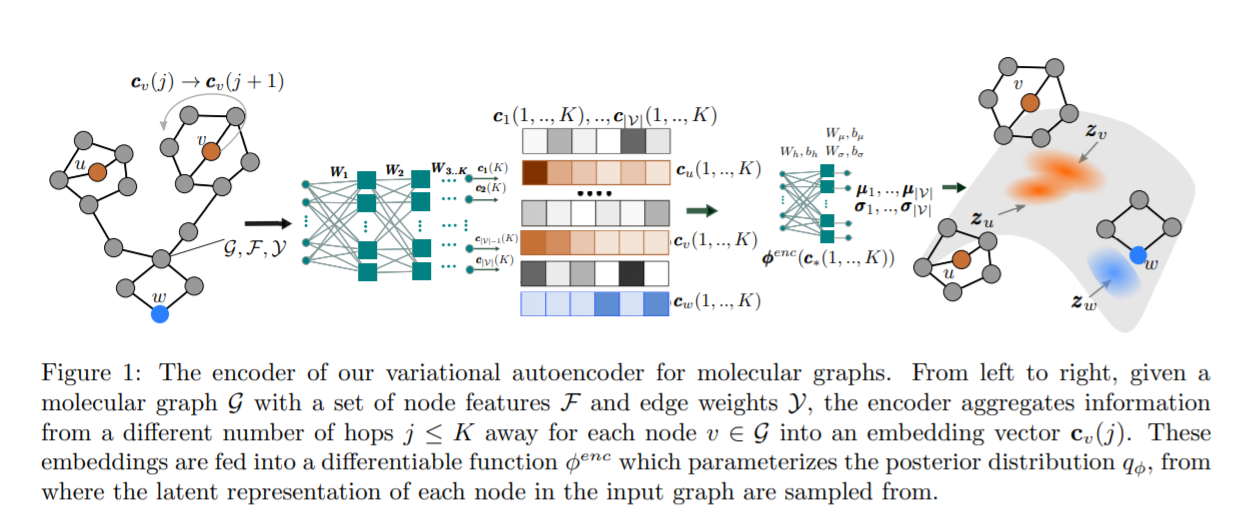
\includegraphics[width=0.85\paperwidth]{nevae-enc.PNG}}

    GNN-like message-passing on k-hops:
    \begin{align}
        &q_\phi(\bs z_u|\mathcal{V,E,F,Y})\sim\mathcal{N}(\bs \mu_u,Diag(\bs \sigma_u))\\
        &[\bs \mu_u, \bs \sigma_u]=\phi^{enc}({\bs c_u(k)}_{k=1..K})\\
        &\bs c_u(k)=
        \begin{cases}
            &\bs r(\bs W_k^\mathcal{T}\bs t_u + \bs W_k^\mathcal{X}\bs x_u),k=1\\
            &\bs r(\bs W_k^\mathcal{T}\bs t_u + \bs W_k^\mathcal{X}\bs x_u\odot \bs \Lambda(\{y_{uv} \bs c_v(k-1)\}_v\in N(u))),k>1
        \end{cases}
    \end{align}

    \subsection{Decoder}
    \centerline{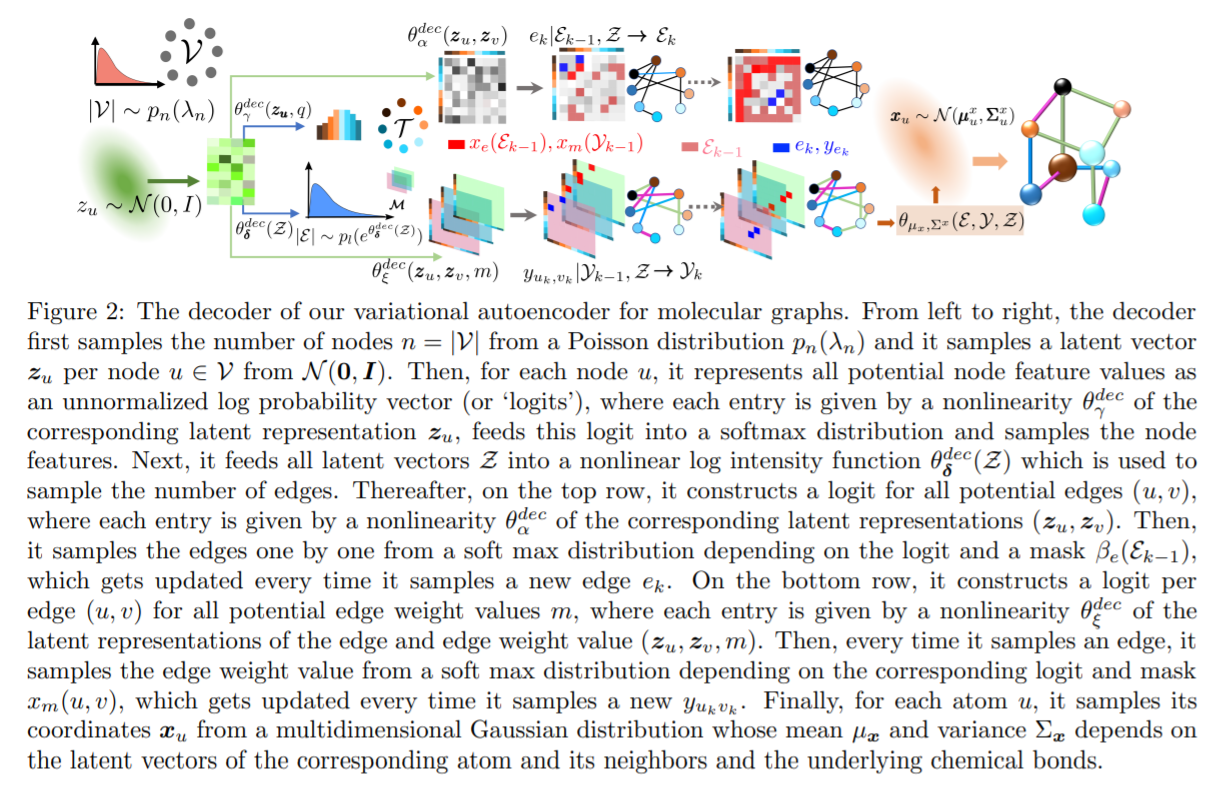
\includegraphics[width=0.85\paperwidth]{nevae-arch.PNG}}

    Decoder: gen. logits, softmax edges one-by-one, possible binary mask(for expert exp.).
    \begin{align}
        &\text{Nodes Count:} |\mathcal{V}|\sim p_l(\lambda_n)\\
        &\text{Latent Repr.:} {\bs z_u}\sim \mathcal{N}(\bs 0,\bs I)\\
        &\text{Node Feat.:} \bs f_u=softmax_u(\theta_{\bs \gamma}^{dec}(\bs z_u, q)),q \text{is atom type}\\
        &\text{Edges Count:} |\mathcal{E}|\sim p_l(e^{\theta_{\bs \delta}^{dec}(\mathcal{Z})})\\
        &\text{Edges Gen.:} p(e=(u,v)|\mathcal{E}_{k-1},\mathcal{V})=\frac{\beta_e e^{\theta^{dec}_{\bs \alpha}(\bs z_u, \bs z_v)}}{\sum_{e'=(u',v')\not \in \mathcal{E}_{k-1}} \beta_{e'} e^{\theta^{dec}_{\bs \alpha}(\bs z_u', \bs z_v')}}\\
        &\text{E. Feat. Gen.:} p(y_{uv}=m|\mathcal{Y}_{k-1},\mathcal{V})=\frac{\beta_m(u,v) e^{\theta^{dec}_{\bs \xi}(\bs z_u, \bs z_v, m)}}{\sum_{m'\not=m \beta_m'(u,v) e^{\theta^{dec}_{\bs \xi}(\bs z_u, \bs z_v, m')}}},\text{note: not normal softmax?}\\
        &\text{Pos. Gen.:} p(\bs x_u|\mathcal{E,Y,Z})=\mathcal N(\bs \mu_x, \bs \Sigma_x)\\
        &[\bs \mu_x, \bs \Sigma_x]=[\theta_{\mu^x}(\bs r(u)), \theta_{\Sigma^x}(\bs r(u))\theta_{\Sigma^x}^T(\bs r(u))]\\
        &\bs r(u)=\bs z_u+\sum_{v\in N(u)}y_{uv}\bs z_v
    \end{align}

    \subsection{Training}
    \begin{itemize}
        \item \bt {Prior}: $\mathcal Z\sim \mathcal N(\bs 0, \bs I)$
        \item maximize evidence lower bound(ELBO)+Poisson max-likelihood:
        \begin{align}
            &\max_{\phi, \theta, \lambda_n} \frac 1 N \sum_{i\in[N]} \mathbb E_{q_\phi(\mathcal Z_i|\mathcal V_i, \mathcal E_i, \mathcal F_i, \mathcal Y_i})[\log p_\theta(\mathcal Y_i, \mathcal E_i, \mathcal F_i, |\mathcal Z_i)] - KL(q_\phi||p_z) + \log p_{\lambda_n}(n_i))
        \end{align}
        \item note term $E_{q_\phi}[\log p_\theta(\mathcal Y_i, \mathcal E_i, \mathcal F_i, |\mathcal Z_i)]$ need the edges sequence specified, use BFS with random tie breaking in child-sel. step, with random selected source node $s\sim \zeta_s$! Thus 
        \begin{align}
            E_{q_\phi}[\log p_\theta(\mathcal Y_i, \mathcal E_i, \mathcal F_i, |\mathcal Z_i)]
            &\approx E_{q_\phi}[\log \mathbb E_{s\sim \zeta_s} p_\theta(\mathcal Y_i, \mathcal E_i, \mathcal F_i, |\mathcal Z_i)] \\
            &\ge E_{q_\phi, s\sim \zeta_s}[ \log p_\theta(\mathcal Y_i, \mathcal E_i, \mathcal F_i, |\mathcal Z_i)]
        \end{align}
        \item \bt{Theorem} If dist. $\zeta_s$ is independent to labels of nodes, then the learned model is permutation-invariant.
        \item \bt{Proposition} Decoder defined is permutation-invariant.
    \end{itemize}

\subsection{Property Oriented Mol. Gen.}
    Train variational probablistic decoder, to maxmize some property of mol., \trarr train a supervised decoder $p^*$ on trained decoder $p_\theta$:
    \begin{align}
        & \min_{p(\cdot|\mathcal Z)} \mathbb E_{\mathcal Z\sim p_z(\cdot)}\mathbb E_{\mathcal{E,Y,F}\sim p(\mathcal{E,Y,F}|\mathcal Z)}[l(\mathcal{E,Y,F})+\rho \log \frac{p(\mathcal{E,Y,F}|\mathcal Z)}{p_\theta (\mathcal{E,Y,F}|\mathcal Z)}]\\
        \Rightarrow &\min \mathbb E_{\mathcal Z\in p_z}[KL(p(\cdot|\mathcal Z)||g_\theta(\cdot|\mathcal Z))]\\
        \text{where } &g_\theta(\mathcal{E,Y,F}|\mathcal Z)=\frac{p_\theta(\mathcal{E,Y,F}|\mathcal Z)\exp(-\frac{l(\mathcal{E,Y,F})}{\rho})}{\mathbb E_{\mathcal{E,Y,F}\sim p_\theta(\cdot|\mathcal Z)} [p_\theta(\mathcal{E,Y,F}|\mathcal Z)\exp(-\frac{l(\mathcal{E,Y,F})}{\rho})]}
    \end{align}

    The above equations has a obvious solution $p^*\equiv g_\theta$, however sampling might be too slow for practical use \trarr A Stochastic Gradient Approach.

    \centerline{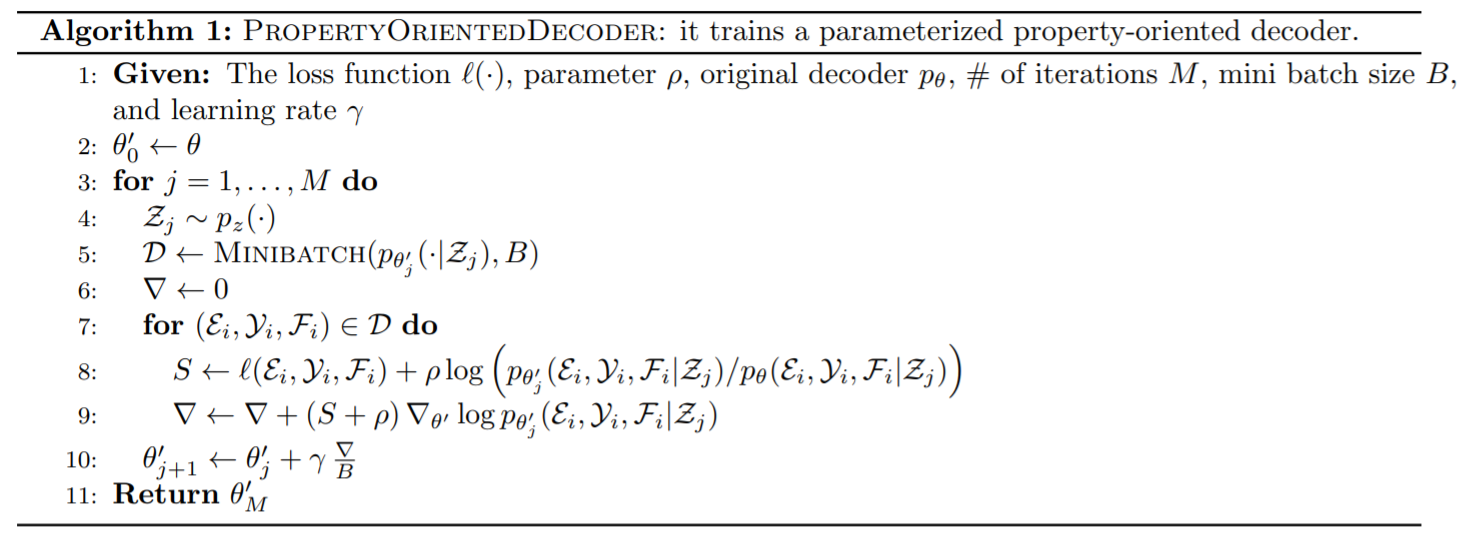
\includegraphics[width=0.85\paperwidth]{nevae-alg1.PNG}}
    Use SGD to update param. $\theta'$ of $p_{\theta'}$:
    \begin{align}
        \Delta \theta' &= \alpha \nabla_{\theta'} \mathbb E_{\mathcal Z\sim p_z(\cdot)}\mathbb E_{\mathcal{E,Y,F}\sim p(\mathcal{E,Y,F}|\mathcal Z)}[l(\mathcal{E,Y,F})+\rho \log \frac{p(\mathcal{E,Y,F}|\mathcal Z)}{p_\theta (\mathcal{E,Y,F}|\mathcal Z)}]\\
        &= \alpha \mathbb E_{\mathcal Z\sim p_z(\cdot)} \nabla_{\theta'} \mathbb E_{\mathcal{E,Y,F}\sim p(\mathcal{E,Y,F}|\mathcal Z)}[l(\mathcal{E,Y,F})+\rho \log \frac{p(\mathcal{E,Y,F}|\mathcal Z)}{p_\theta (\mathcal{E,Y,F}|\mathcal Z)}]\\
        \text{(by log-deriv. trick) } &= \alpha \mathbb E_{\mathcal Z\sim p_z(\cdot)} \mathbb E_{\mathcal{E,Y,F}\sim p(\mathcal{E,Y,F}|\mathcal Z)}\left[
            (l(\mathcal{E,Y,F})+\rho \log \frac{p(\mathcal{E,Y,F}|\mathcal Z)}{p_\theta (\mathcal{E,Y,F}|\mathcal Z)}+\rho)\nabla_{\theta'} \log p_{\theta'}
        \right]
    \end{align}
    by a unbiased MC estim.
    \begin{align}
        &\approx \frac {1}{M} \sum_{i\in[M]}
        \left[
            (l(\mathcal{E,Y,F})+\rho \log \frac{p(\mathcal{E,Y,F}|\mathcal Z)}{p_\theta (\mathcal{E,Y,F}|\mathcal Z)}+\rho)\nabla_{\theta'} \log p_{\theta'}
        \right]
    \end{align}


\section{Seminar on Self/Un-Supervised Learning @ 2020/9/16}
\subsection{Self-Learning @ Video Learning}
    Supervised success: good \& sufficient data, a way different from human! \tRarr \textit{Linda Smith, The Dev. of Embodied Cognition}

    \bt{Paragidims}:
    \begin{itemize}
        \item Use proxy task(e.g. semantics repr.) for a repr., use linear probing for downstream task.
        \item Use proxy task(e.g. semantics repr.) for a repr., generalizable with \textit{zero annotation}
    \end{itemize}
    
    \bt{Why video-based self-supervised}: like what human percepts, rich info; might with audio.

    Proxy loss design: temporal info, spatial cohenrence, motions of obj., multimodal
    
    \bt{Temporal}:
    \begin{itemize}
        \item shuffle \& learn
        \item forward or backward?(arrow of time)
        \item SpeedNet: which speed(frame-rate) is normal/speed-up 
        \item ===Weak, irrelative with downstream tasks===
        \item DPC: \textit{learn repr. in predicting future in video}
    \end{itemize}

    \centerline{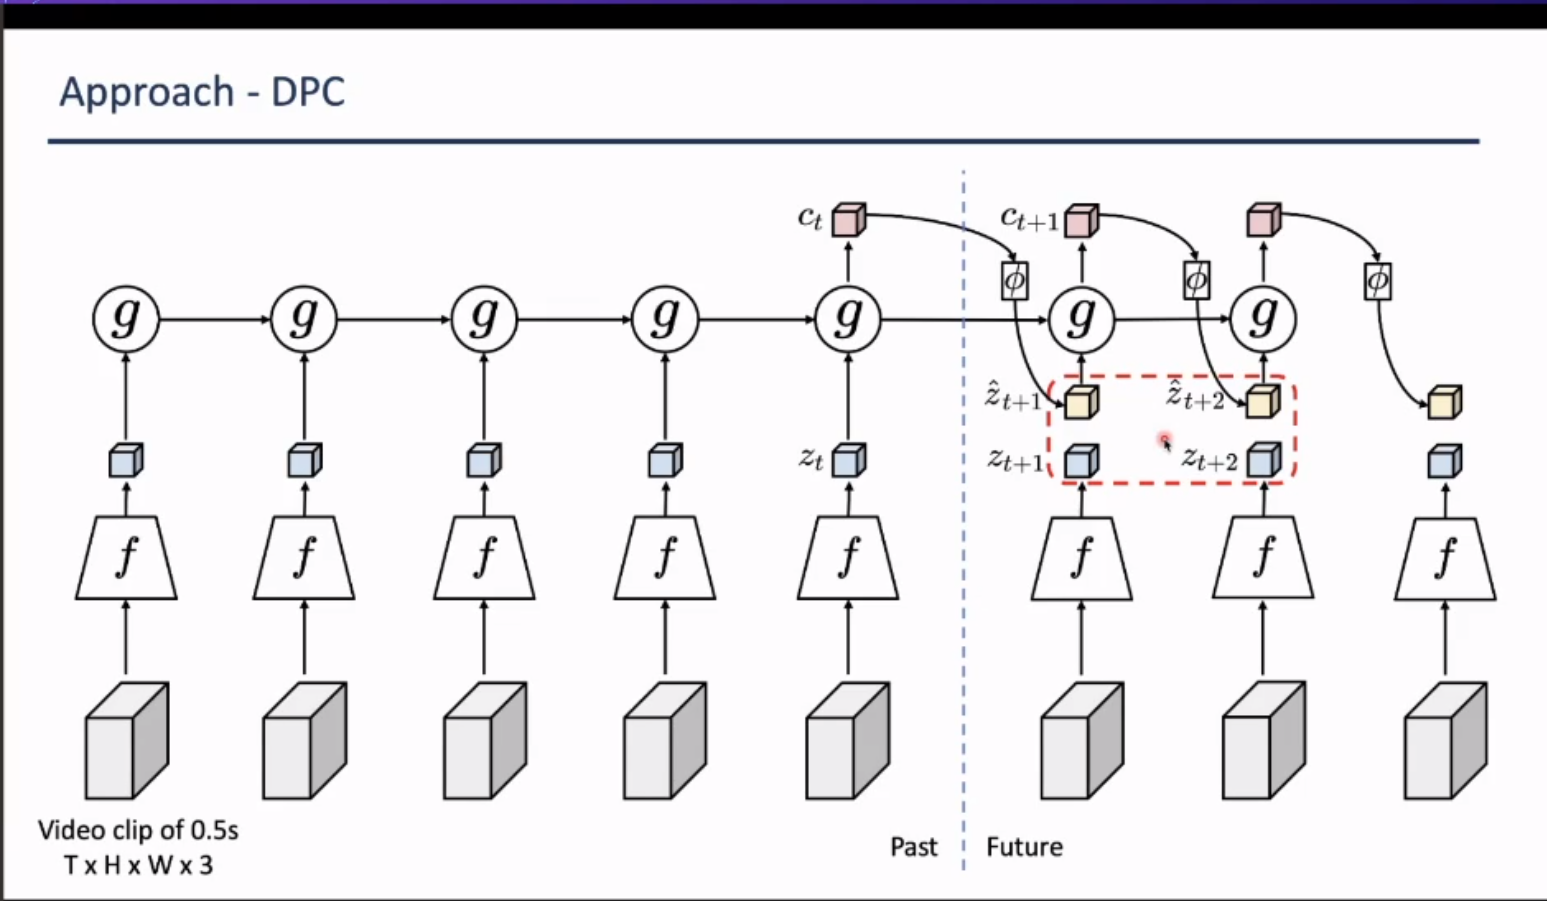
\includegraphics[width=0.8\paperwidth]{dpc-arch.PNG}}
    DPC Arch.:encoder-decoder like, contrast learning(infoNCE)

    \centerline{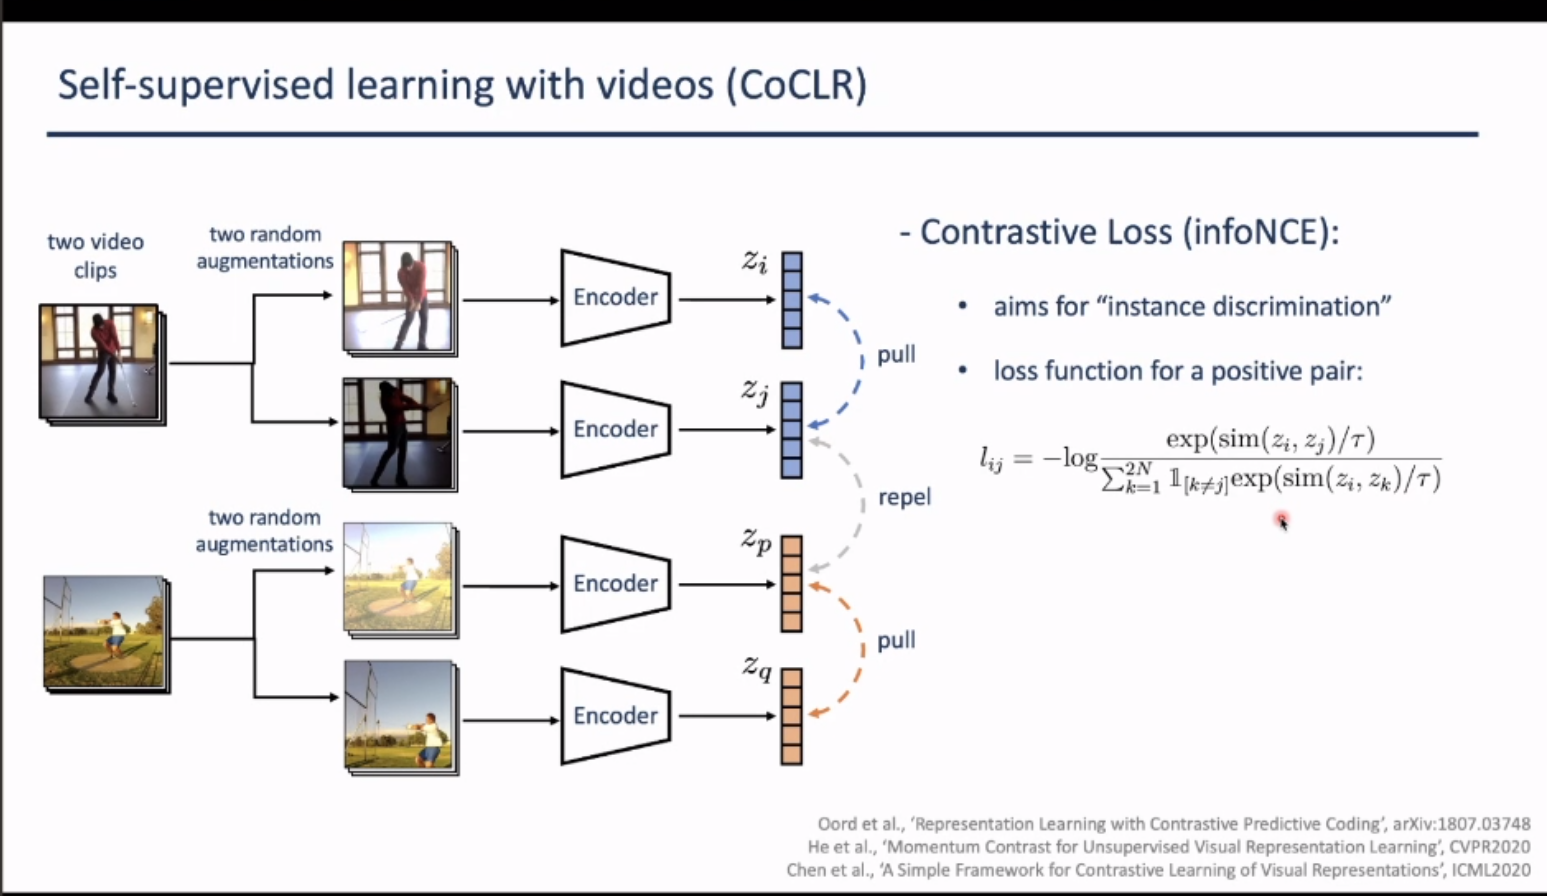
\includegraphics[width=0.8\paperwidth]{coclr.PNG}}
    \centerline{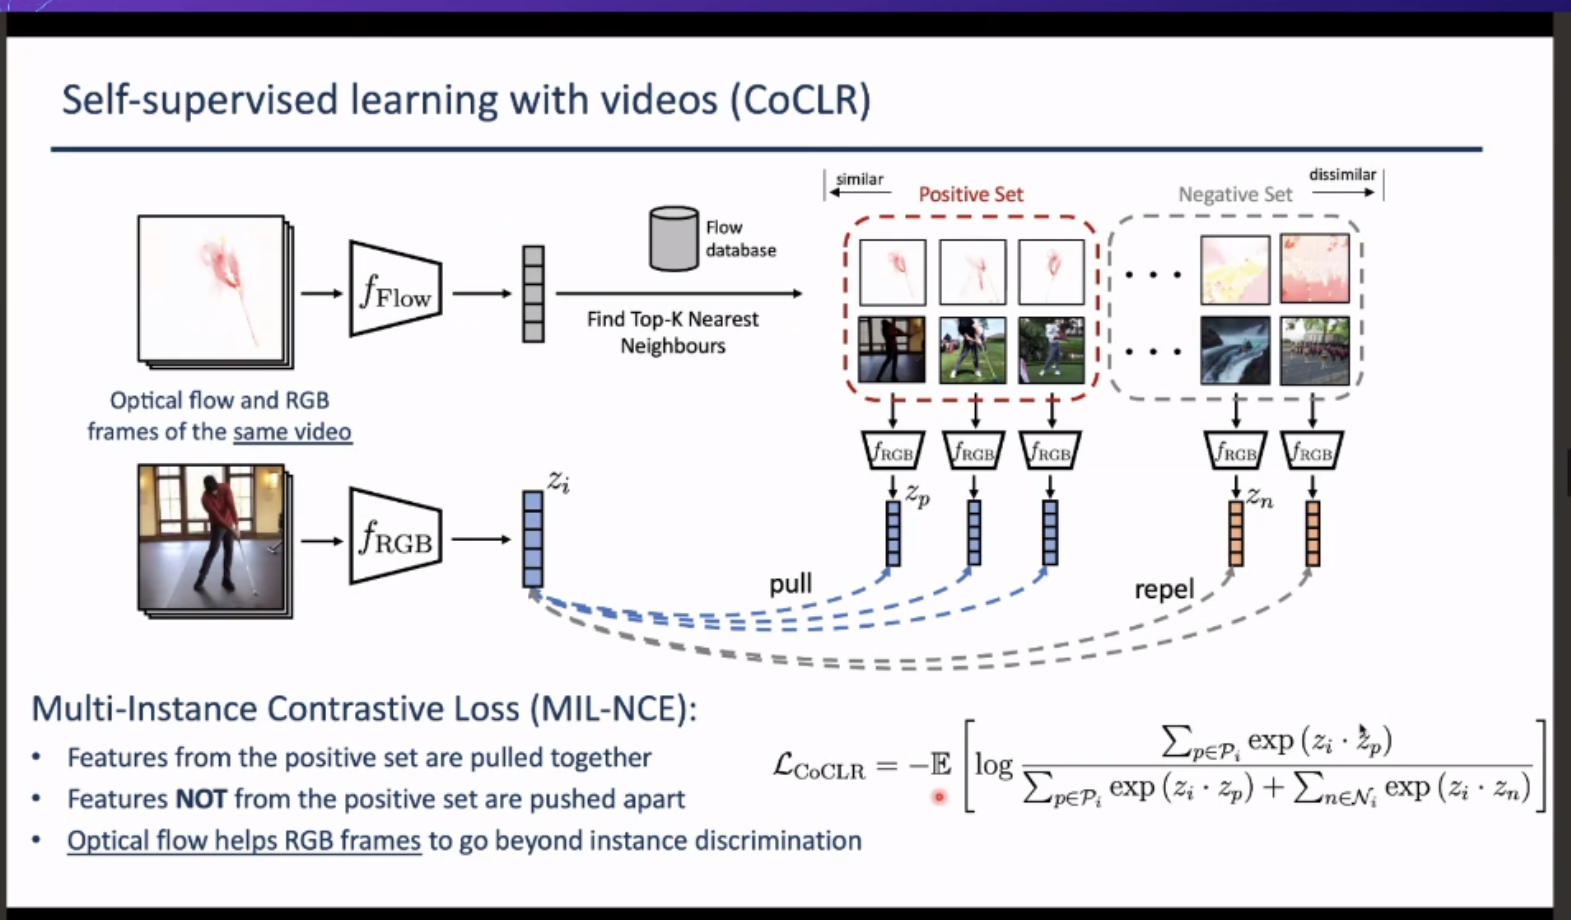
\includegraphics[width=0.8\paperwidth]{coclr2.PNG}}
    CoCLR: SimCLR like(infoNCE), colearning multimodally with motion flow(MIL-NCE, with noise added)

    Audio-Video Co-learning: train a net to check if image/audio clip are same-sourced! Get both video/audio repr.

    MAST: self-supervised tracking, give 1st frame mask(seg.), predict sequantial segmentations

    \bt{Next}:
    \begin{itemize}
        \item More efficient learning
        \item Scale up model to uncurrated data, like GPT-1/2/3
        \item Design proxy task for obj-centric learing
        \item Design and understand \bt{effective memory!!!}(for video task especially)
        \item Hand-crafted proxy task \trarr Auto proxy task design?
        \item Theoratic: small or negative improvement, in upstream task to downstream task.
        \item Are there difficult task for supervised learning but easy for SSL(e.g. unable to label)?
    \end{itemize}

\subsection{Transformation Equivariance vs. Invariance @ Visial Repr. Learning}
    \bt{Contents}:
    \begin{itemize}
        \item TER(Transformation Equivariance Repr.)
        \item AET(AutoEncoding Transformation)
        \item AVT(Autoencoding Variational Transformation)
        \item SAT(Semi-supervised Autoencoding Transformation)
    \end{itemize}

    CNN = Translation Equivariant Repr. + FC Classifier. Go beyond: Tranformation Equivariant Repr. + Tranformation Invariant Classifier

    Trans. Equiv.: $E(\bs t(\bs x))=\bs \rho(\bs t)[E(\bs x)]$. Trans. Inv. is when $\bs \rho \equiv \bs 1_E$.

    Steerability: $\bs \rho$ is inpend. with sample $\bs x$.

    Targets: Non-linear $\bs \rho$, General Transformation(e.g. recoloring)

    % \centerline{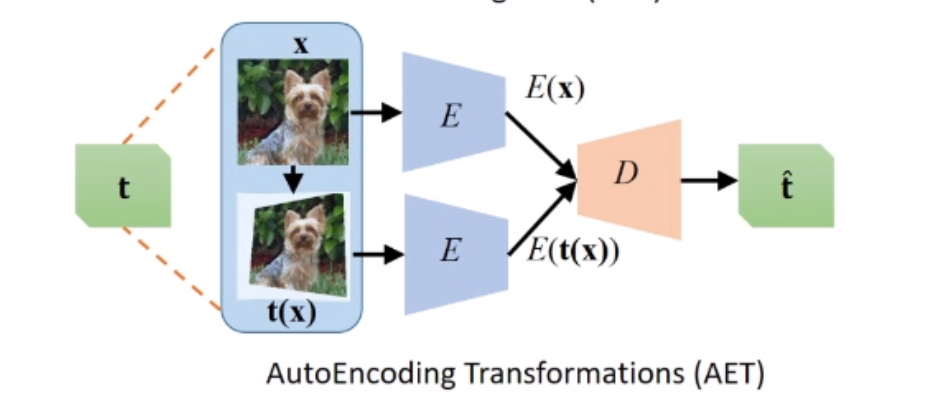
\includegraphics[width=0.8\paperwidth]{aet.PNG}}
    % \centerline{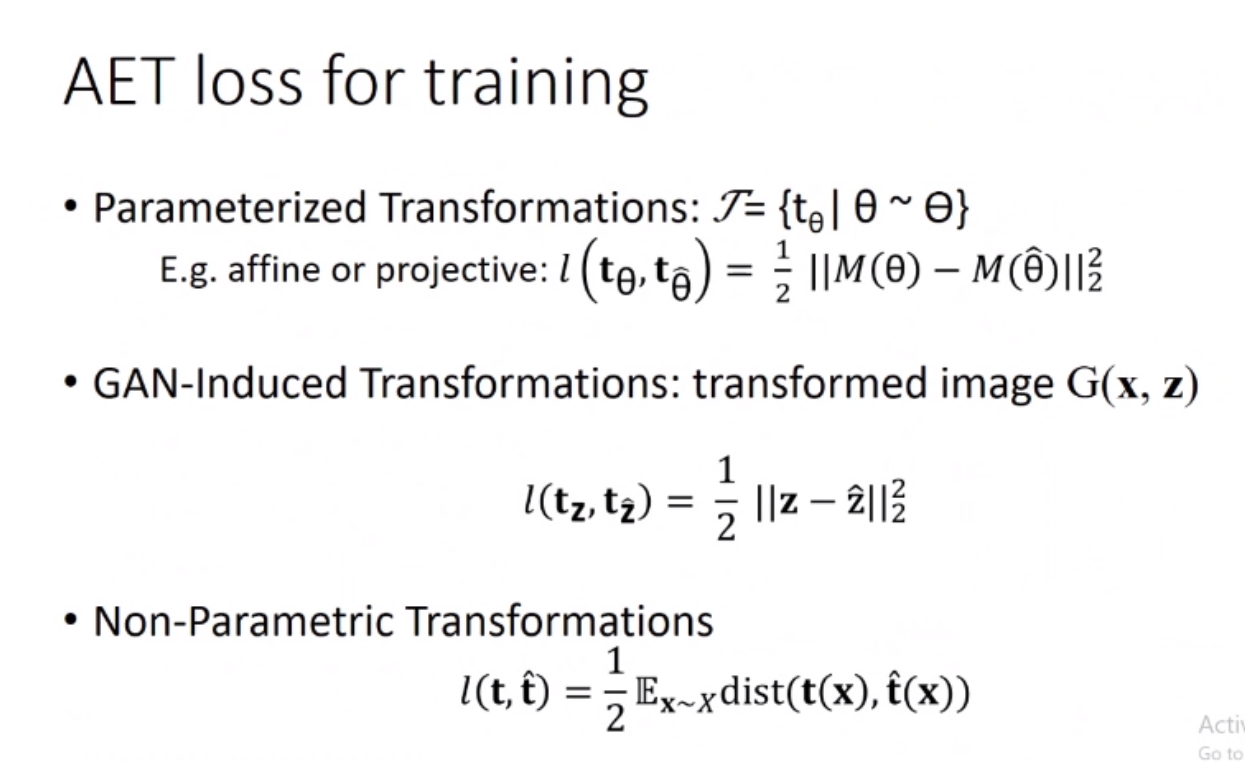
\includegraphics[width=0.8\paperwidth]{aetloss.PNG}}
    % AET:\begin{itemize}
    %     \item use autoencoders to learn \bt{transformations}
    %     \item trans. generated randomly for self-supervised learing
    %     \item use Siamese net as encoder backbone
    %     \item AET loss: parameterized, non-parametric, GAN-induced
    % \end{itemize}
    
    % \centerline{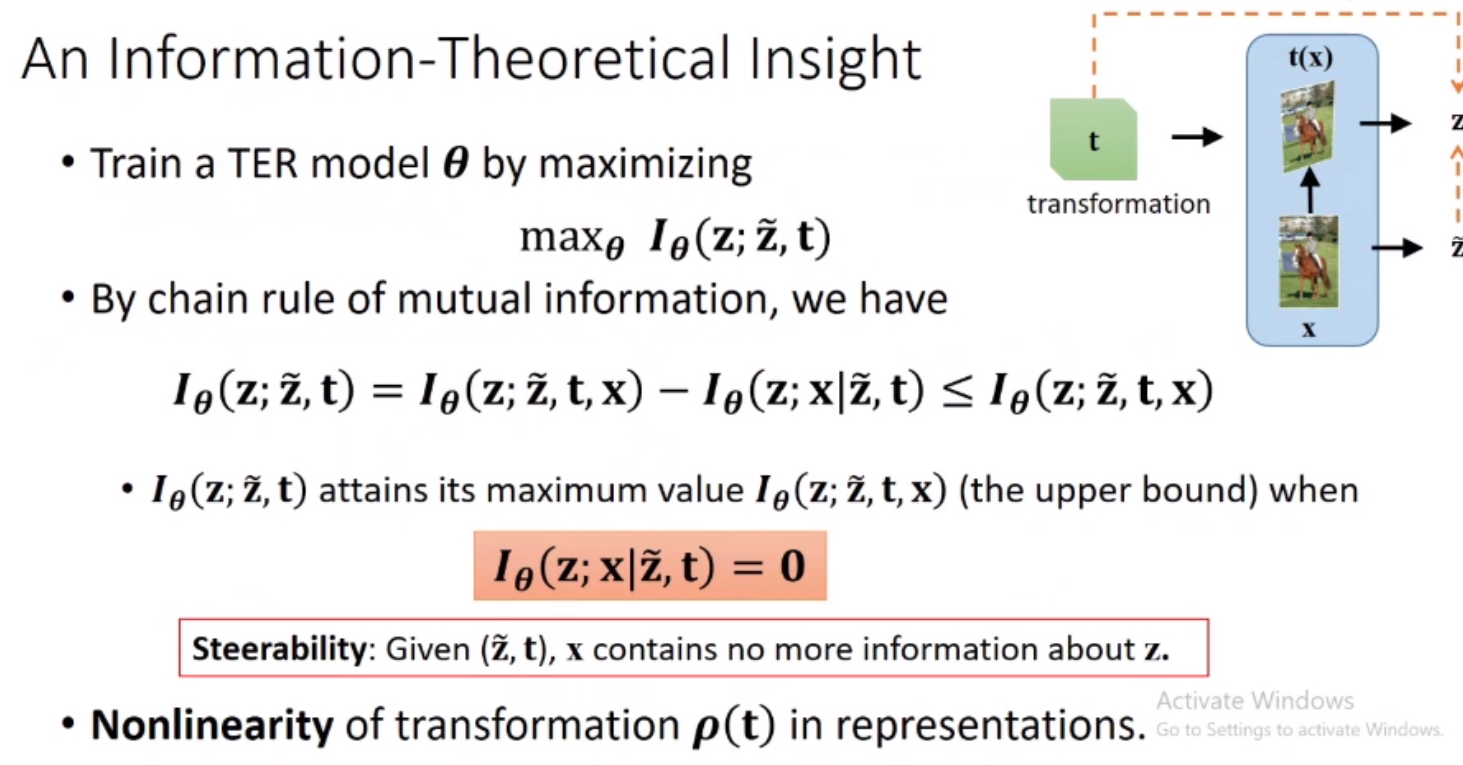
\includegraphics[width=0.8\paperwidth]{avt.PNG}}
    % \centerline{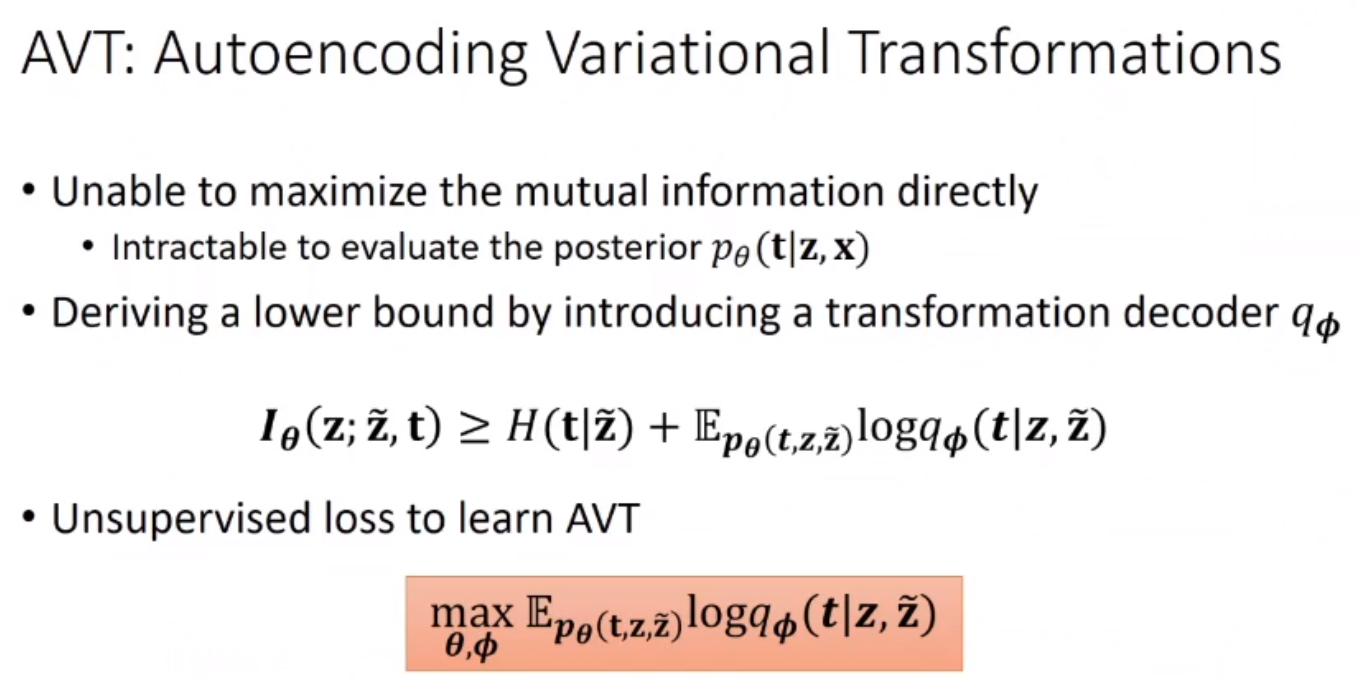
\includegraphics[width=0.8\paperwidth]{avt2.PNG}}
    % \centerline{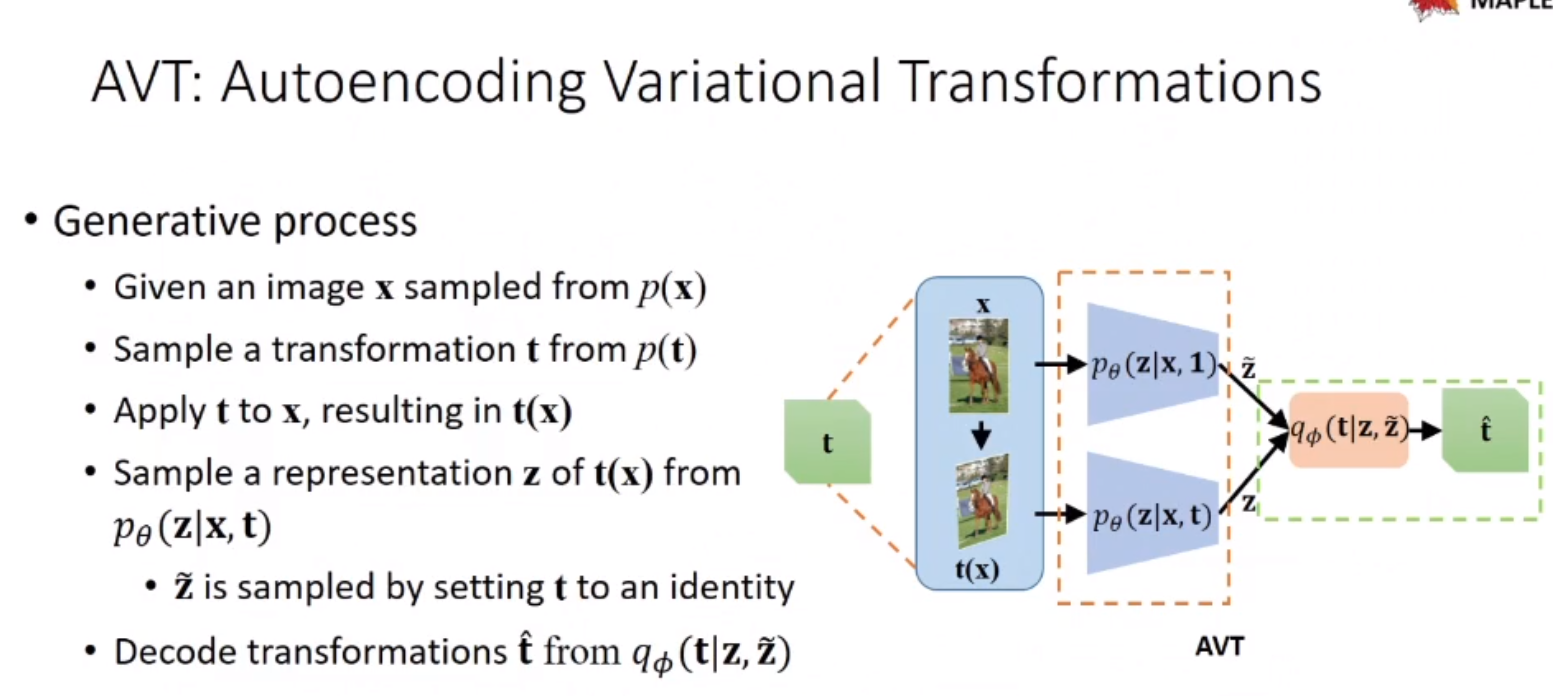
\includegraphics[width=0.8\paperwidth]{avt-training.PNG}}
    % AVT:
    % \begin{itemize}
    %     \item minimize $z, x$ mutual info \trarr maxmize $I_\theta(z; \tilde z, t)$
    % \end{itemize}

    \centerline{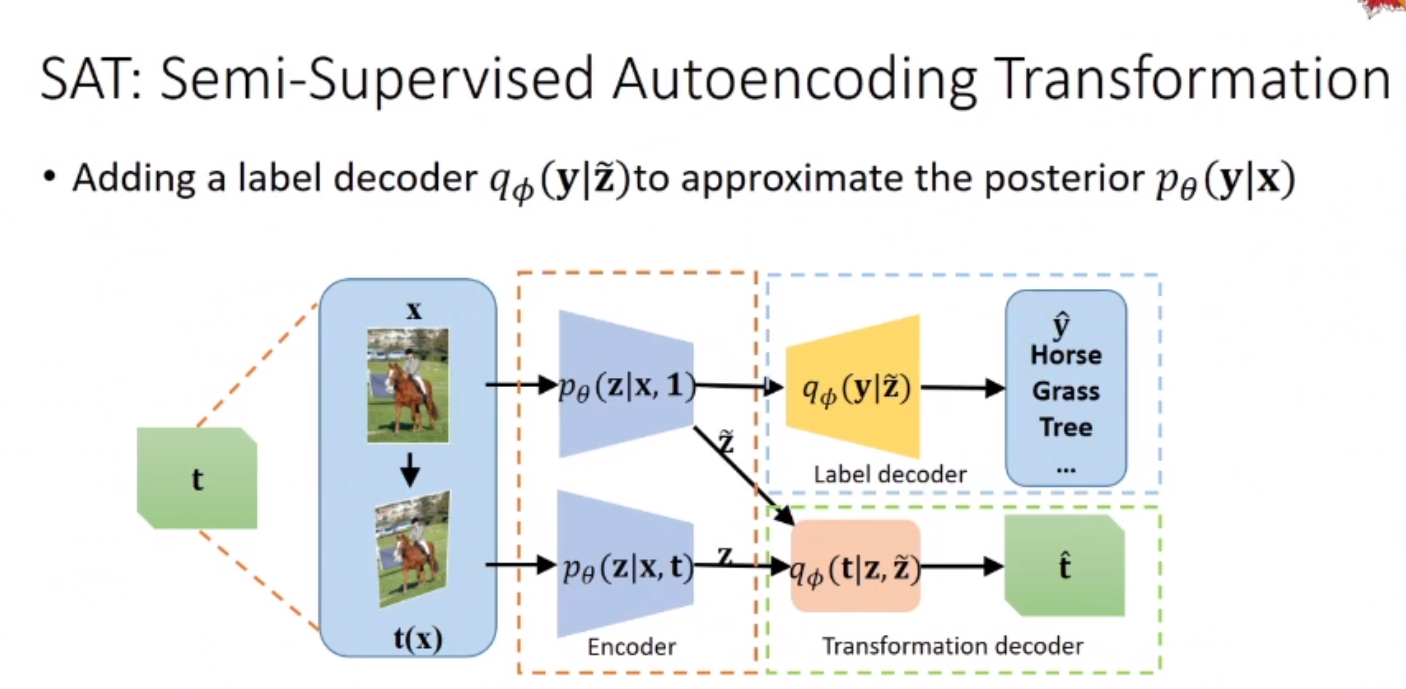
\includegraphics[width=0.8\paperwidth]{sat.PNG}}
    \centerline{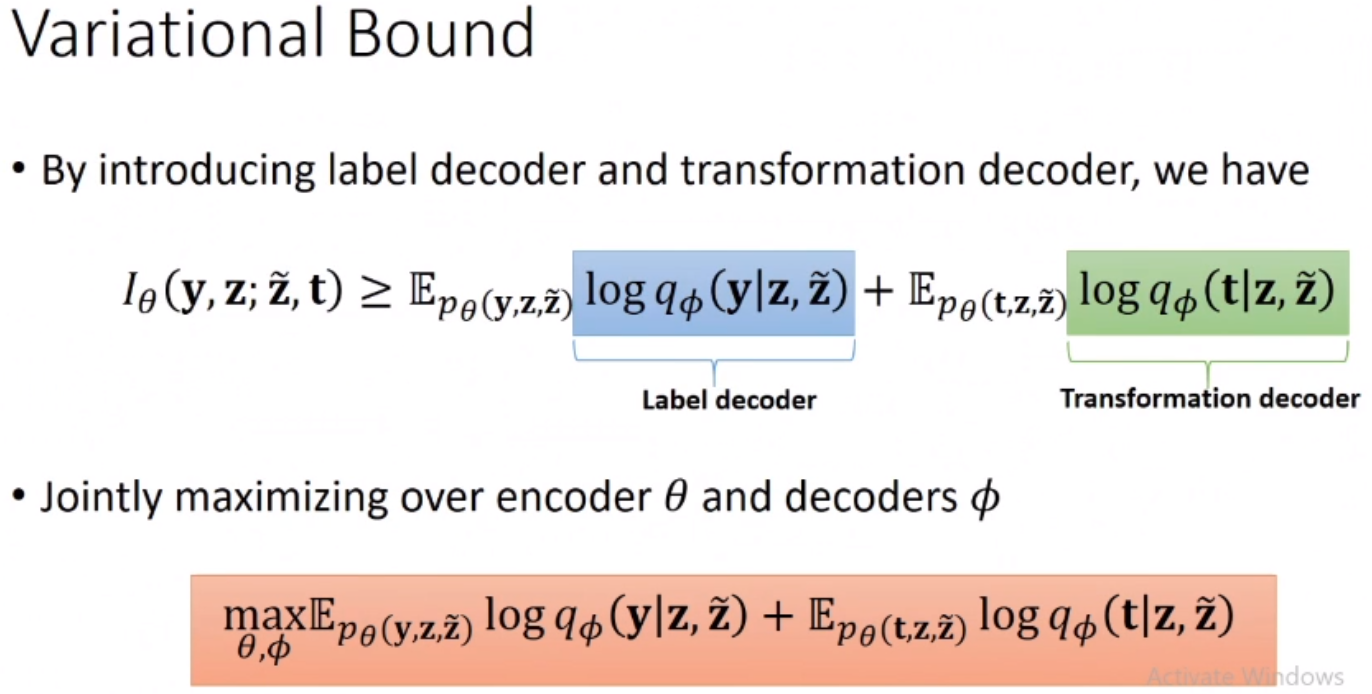
\includegraphics[width=0.8\paperwidth]{sat-loss.PNG}}
    SAT:
    \begin{itemize}
        \item add a label decoder compared to AVT.
        \item variational surrogate \trarr cross-entropy loss on supervised data + AVT loss
    \end{itemize}

    Contrastive Learning: more utilized trans-invariant repr.
    Future: unifying trans-inv/equiv repr.

\section{AET, AVT: Autoencoding Transformations}

    \bt{Idea} autoencoders used in modeling transformations rather than images in order to learn general repr.

    \centerline{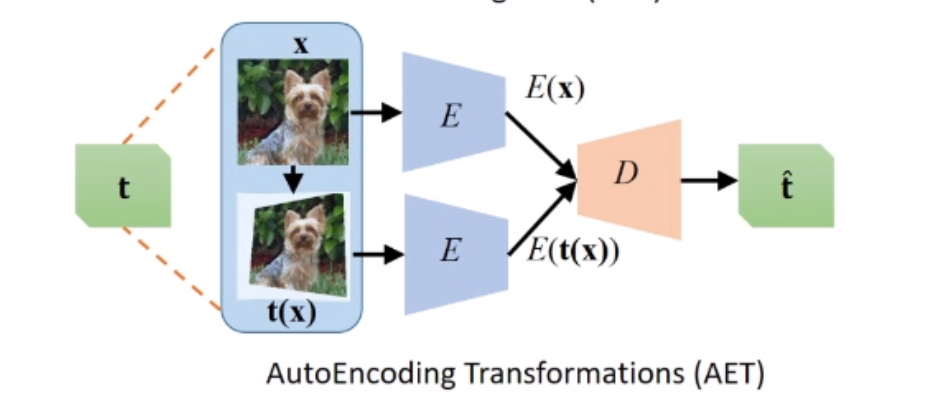
\includegraphics[width=0.8\paperwidth]{aet.PNG}}
    AET:\begin{itemize}
        \item use autoencoders to learn \bt{transformations}
        \item trans. generated randomly for self-supervised learing
        \item use Siamese net as encoder backbone
        \item AET loss: parameterized, non-parametric, GAN-induced
    \end{itemize}
    Losses in AET:
    \begin{itemize}
        \item parameterized transformations: if trans. are parameterized $\mathcal T \in \{t_\theta | \theta \in \Theta\}$, loss can be defined as norm of param. diff. 
        $$l(t_\theta, t_{\hat \theta}=||\theta - \hat \theta||_{\cdot})$$
        \item for non-parametric trans., use expected distance on source domain 
        $$l(t, \hat t)=\mathbb E_{x\sim X}\{dist(t(x), \hat t(x)))\}$$
        \item GAN-induced trans.: image tranformed in form $G(x, z)$, we have loss 
        $$l(t_z, t_{\hat z}=||z-\hat z||_\cdot)$$
    \end{itemize}

    \bt{Idea of AVT} use prob. dist. to model trans., VAE like modeling!
    
    \centerline{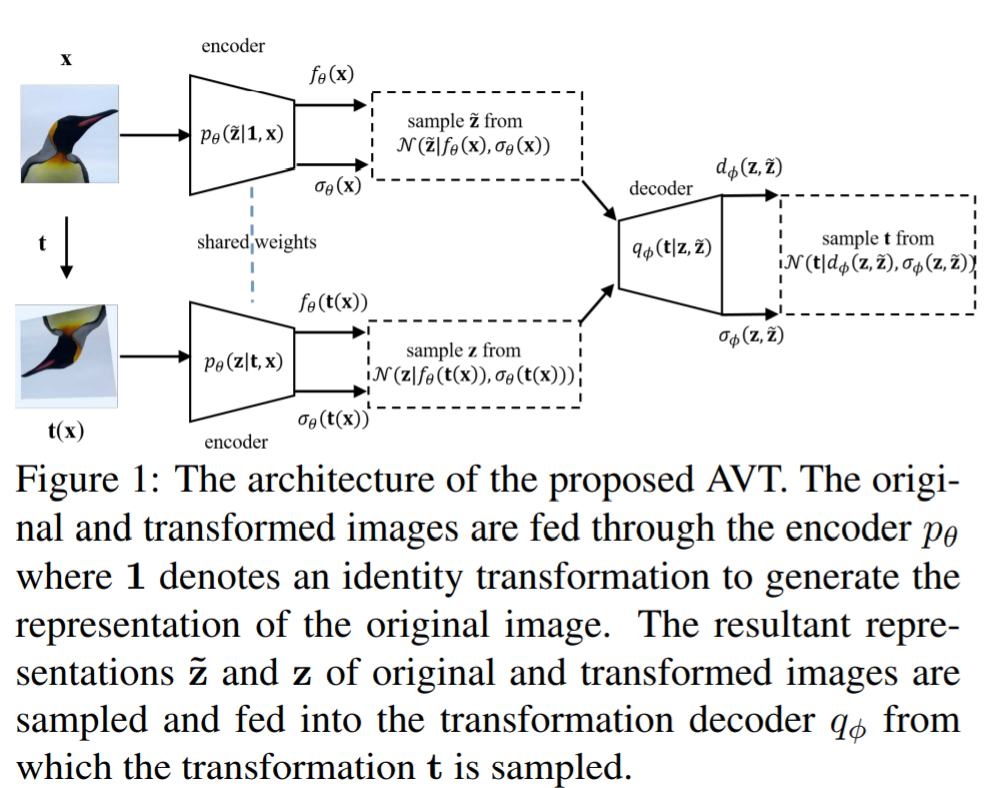
\includegraphics[width=0.8\paperwidth]{avt-arch.PNG}}
    AVT: \begin{itemize}
        \item maximize mutual info $I(t;z|\tilde z)$
        \item variational bound, introdicing a decoder $q_\phi(t|z, \tilde z)$:
            \begin{align}
                I(t;z|\tilde z) &= H(t|\tilde z) - H(t|z, \tilde z)\\
                &= H(t|\tilde z) + \mathbb E_{p_\theta(t, z, \tilde z)}[p_\theta(t|z,\tilde z)]\\
                &= H(t|\tilde z) + \mathbb E_{p(t, z, \tilde z)}[q_\theta(t|z,\tilde z)] + \mathbb E_{p_(z, \tilde z)}[D(p_\theta(t, z, \tilde z)||q_\phi(t|z,\tilde z))]\\
                &\ge H(t|\tilde z) + \mathbb E_{p(t, z, \tilde z)}[q_\phi(t|z,\tilde z)]\equiv \tilde I(t;z|\tilde z)\\
                &\Rightarrow \max_{\theta,\phi} \mathbb E_{p(t, z, \tilde z)}[q_\phi(t|z,\tilde z)]
            \end{align}
        \item specifically in batch-wise formulation:\begin{align}
            &\mathbb E_{p(t, z, \tilde z)}[q_\phi(t|z,\tilde z)]\approx \frac 1 n \sum_{i=1}^n \log \mathcal N(t^i|d_\phi(z^i, \tilde z^i), \sigma_\phi(z^i, \tilde z^i))\\
            &\text{where }z^i=f_\theta(t^i(x^i))+ \sigma_\theta(t^i(x^i))\odot \epsilon^i\\
            &\text{and }\tilde z^i=f_\theta(x^i)+ \sigma_\theta(x^i)\odot \tilde \epsilon^i\\
            &\text{where }\epsilon^i, \tilde \epsilon^i \sim \mathcal(\epsilon|0,I), t^i\sim p(t)\text{(predifined or so?)}
        \end{align}
        \item trick: take 5 samples to full explore the distribution 
    \end{itemize}

\section{Flow-Based Generative Models}

\subsection{Outline \& Basics}

    Two random vector of same dim.: 
    \begin{align}
        &X\sim P_X(x), z\sim \Pi_Z(z), \text{find mapping } f:Z\rightarrow X=x(z), 
    \end{align}
    we have 
    \begin{align}
        \begin{cases}
            p_X(x)=\pi_Z(f^{-1}(x))\left|\det J(f)\right|^{-1}\\
            \pi_Z(z)=p_X(f(z)))\left|\det J(f)\right|
        \end{cases}
    \end{align}
    use a simple dist. on $Z$ and invertibly generate $X\sim p_G(x)$: $x=G(z)$. train $G^{-1}$ as a discriminator.
    keys: invertible, easy-to-compute $G^{-1}$, easy-to-compute Jacobian determinant.

    \bt{``Coupling Layer"}:
    \begin{align}
        &\begin{cases}
            \text{(copy)} x_i = z_i, i\le d\\
            \text{(affine)} x_i = \beta_i z_i + r_i, d < i \le D
        \end{cases}\\
        & \beta_{d+1,...D}=F(z_{d+1,...D}), \gamma_{d+1,...D}=H(z_{d+1,...D})\\
        & J_G=\left[\begin{array}{c|c}
            \bs I_d &\bs O\\
            \hline\\
            \bs M\text{(non-matter)} &\bs D\text{(diagonal)}
        \end{array}
        \right]\\
        & \det J_G = \prod_{k=d+1..D}\frac{\partial x_k}{\partial z_k}
    \end{align}

    Use many coupling layer to enhance expessive capability. Parts of image does not change \trarr exchange copy/affine split:
    \begin{itemize}
        \item exchange within channel
        \item exchange channel \trarr channel rotation use matrix/$1\times 1$ convolution in MoFlow
    \end{itemize}
\subsection{MoFlow}

    \bt{Summary} Flow-based on molecular graphs, channel rotation as $1\times 1$ convolution, relational GCN layer, graph conditional flow(GCF), use sigmoid rather than exp, split dimensions.

    \bt{``Coupling Layer"}:
    \begin{align}
        &Z_{1:d} = X_{1:d}\\
        &Z_{d+1:n} = X_{d+1:n} \odot sigmoid(S_\Theta(X_{1:d}))+T_\Theta(X_{1:d})
    \end{align}
    here $S \sim $ scaling, $T \sim$ translation, both by DNNs.每个耦合层交换上一层copy的dims, 通过一个channel上的旋转 $W\in \R^{c\times c}$,等价于一个1*1卷积, 变换后的Y分为$(Y_{1:c/2}, Y_{c/2+1,n})$送入下一层. 采用split-dims的trick,增加交换channel的模型自由度增加: $X\in \R^{c\times n \times n}\Rightarrow \R^{ch^2\times n/h \times n/h}$

\subsubsection{GCF/Graph Conditional Flow}

    \centerline{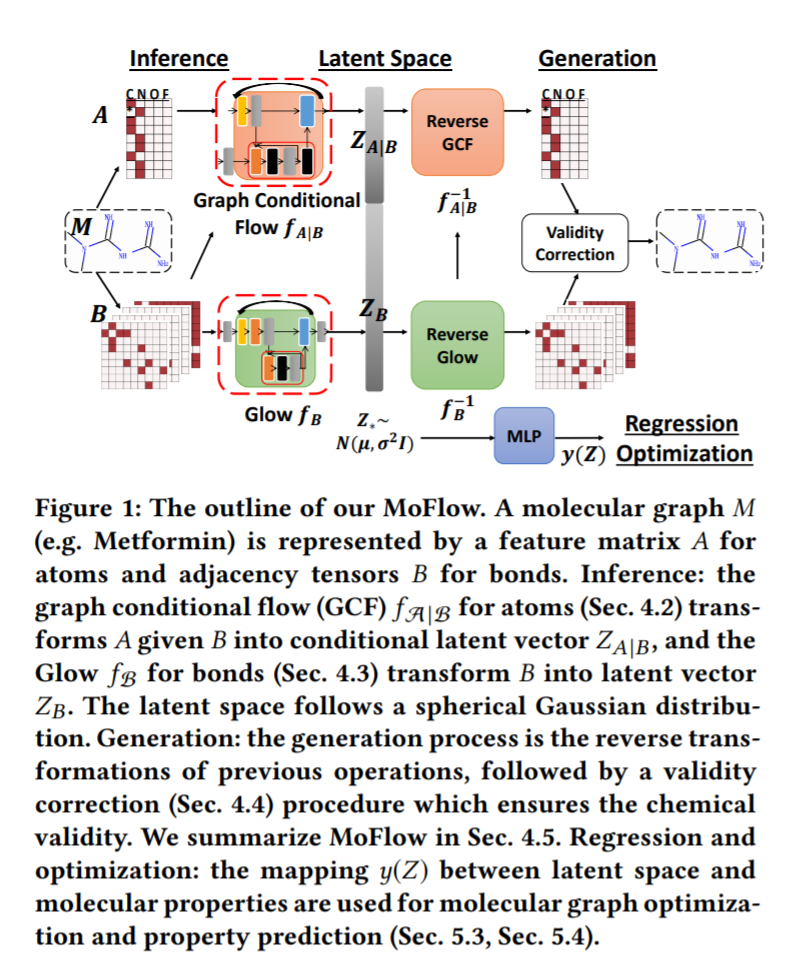
\includegraphics[width=0.85\paperwidth]{moflow-arch.PNG}}
    \bt{Def.(B conditioned flow)} \dots. 

    We have \begin{align}
        J_{A|B} &= \frac{\partial f_{A|B}}{\partial (A,B)}=
        \left[\begin{array}{c|c}
            \frac{\partial f_{A|B}}{\partial A} &\frac{\partial f_{A|B}}{\partial B}\\
            \hline\\
            \bs O & \bs I
        \end{array}\right]\\
        \det J_{A|B} &= \det \frac{\partial f_{A|B}}{\partial A}
    \end{align}

    GCF layer:
    \begin{align}
        & Z_{A|B} = (Z_{A_1|B},Z_{A_2|B}), A=(A_1|A_2)\\
        &\begin{cases}
            \text{\bt{copy} }Z_{A_1|B}=A_1\\
            \text{\bt{affine} }Z_{A_2|B}=A_2\odot sigmoid(S_\Theta(A_1|B)) + T_\Theta(A_1|B)
        \end{cases}
    \end{align}

    Special designed $S, T$ using R-GCN:
    \begin{align}
        &graphconv(A_1) = \sum_{i=[C]} \tilde B_i(M\odot A) W_i + (M\odot A) W_0, \text{where } M \text{ is the mask of split},\\
        &\tilde B \text{ is normalized } \bs B_i: \tilde B_i = \bs D^{-1} \bs B_i, \\
        &\text{where } \bs D \text{ is the full deg-mat. } \bs D = \sum_{c, i} \bs B_{c,i,j} = \sum_c \bs D_i, \text{ computed only once!}
    \end{align}

\subsubsection{Validity Correction \& Misc}

    使用价约束
    \begin{align}
        &\sum_{c,j} c\times B_{c,i,j} \le Valency_i+Ch_i, \text{where $Ch_i$ is formal charge}\\
    \end{align}
    具体的有效性校验方法:
    \begin{enumerate}
        \item 检查价约束,满足去2,否则去3
        \item 返回最大连通子图
        \item 第i个原子不满足,对于第i个原子,删去最高阶键,去1
    \end{enumerate}
    这种方法试图再分子上做最小修改来满足价约束.

    \bt{Note} 为了防止学到的prob. dist. 退化, 在数据集上增加dequantization, 每个dim加噪声$\sim U[0, 0.6]$



\subsection{GraphNVP}

\section{WGAN}

    \bt{Idea} Wasserstain距离代替KL/JS距离.

    \bt{Method} \begin{itemize}
        \item 判别器不用sigmoid, loss不取log
        \item 判别器参数截断 \trarr 为了让判别器Lipschitz连续.
        \item trick: 不用基于momentum的优化器(Adam etc.), 用RMSProp/SGD.
    \end{itemize}

\section{GMMN+AE}
\subsection{Structure \& Idea}
    \centerimage{0.85}{gmmn-arch.png}

    Use MMD(Maximum Mean Discrepency) loss:
    \begin{align}
        L_{MMD^2}&=||\frac 1 N \sum_i \phi(x_i) - \frac 1 M\sum_j \phi(y_j)||^2\\
        &=\frac 1 {N^2} \sum_{i,i'} K(x_i, x_{i'}) + \frac 1 {M^2} \sum_{i,i'} K(y_i, y_{i'}) - \frac{1}{NM} \sum_{i,j} K(x_i, y_j)
    \end{align}
    使用k阶多项式作为核, 则等价于匹配k阶矩!\trarr 使用高斯核,以匹配所有阶矩(看作幂级数),这也是GMMN的名字由来(Moment-Matching):
    \begin{align}
        &K(x, y) = \exp(-\frac{1}{2\sigma} ||x-y||^2)
    \end{align}
    设生成的数据为$(x_i^s)$,gt. 为$(x_i^d)$, 则偏导
    \begin{align}
        &\frac{\partial L_{MMD^2}}{\partial x^s_{ip}} = 
        \frac{1}{\sigma} \left(
            \frac{2}{M^2} \sum_{j=[M]}K(x_i^s, x_j^s)(x_{jp}^s-x_{ip}^s) - 
            \frac{2}{NM} \sum_{j=[N]}K(x_i^s, x_j^d)(x_{jp}^d-x_{ip}^s) 
        \right) 
    \end{align}
\subsection{Training}
    \begin{enumerate}
        \item 逐层训练AE
        \item Finetune AE 
        \item 训练GMMN
    \end{enumerate}

\section{FoldingNet - An AntoEncoder}
    \centerimage{0.85}{foldingnet-arch.PNG}
    
    使用(扩展的)Chamfer距离
    \begin{align}
        &d_{CH}(S, \widehat S)=\max\{
            \frac{1}{|S|} \sum_{x\in S} \min_{x\in \widehat S} ||x-\widehat x||,
            \frac{1}{|\widehat S|} \sum_{x\in \widehat S} \min_{x\in S} ||x-\widehat x||
        \}
    \end{align}
    这个距离让两个点云的点互相配准.

    使用基于图的Encoder:使用的特征为局部(KNN上的)协方差\footnote{
        回忆协方差公式\[
            \cov(\bs X) = \bb E[(\bs X-\bb E \bs X)(\bs X-\bb E \bs X)^T]  
        \]    }+位置($n\times 12$),简要结构: MLP+GNN-Aggregation+MLP\trarr Codeword
    其中Graph Layers
    \begin{align}
        &\bs Y = \bs A_{\max}(\bs X)\bs K\\
        &\bs A_{\max}(\bs X)_{ij} = ReLU(\max_{k\in \mathcal N(i)} x_{kj})
    \end{align}

    基于折叠的Decoder:重复m次codeword, 和$2d$格点concat送到MLP(1st-folding)得到中间折叠点云, 和codeword concat之后再送到第二个folding-mlp中得到结果.

    \bt{Prop.} Encoder proposed is permutation-invariant.

    \bt{Prop.} Decoder proposed can shape arbitrary point cloud.

\section{PointFlow: Flow-based Generative Model on Point Clouds}

    \bt{Idea} As Title
\subsection{Continuous Normalizing Flow(CNF)}
    正则化流, 通过一系列可逆变换$f_i$:
    \begin{align}
        x &= f_1 \circ \dots \circ f_n (y)\\
        \log P(x) &= \log P(y) - \sum_i \left|
            \log \det \cal J_{f_i}
        \right|
    \end{align}

    离散的正则化流被推广到连续的正则化流---CNFs
    \begin{align}
        \frac{\partial y(t)}{t} &= f(y(t), t)\\
        \text{Thus } &=y(t_0) + \int^{t_1}_{t_0}f(y(t),t)dt, y(t_0) \sim P(y)\\
        \log P(x) &= \log P(y(t_0)) - \int^{t_1}_{t_0}\cal Tr(\frac{\partial f}{\partial y(t)})dt 
    \end{align}
    一个黑盒ODE求解器可以用于估计流的输出和输入的梯度!

\subsection{Variational Auto-Encoder}

    Optimize ELBO
    \begin{align}
        \log P_\theta(X) & \ge \log P_\theta(X) - D_{KL}(Q_\phi(z|X)||P_\theta(z|X))\\
        &= \bb E_{Q_\phi(z|X)}[\log P_\theta(X|z)]- D_{KL}(Q_\phi(z|X)||P_\psi \theta(z))
    \end{align}

\subsection{Model}

    \centerimage{0.85}{pointflow-arch.PNG}

    \bt{Summary} VAE-like. Decoder: Flow-based, i.e. CNF; Prior: CNF-based; Encoder: some simple permutation-invariant encoder.

    \bt{Notations}
    \begin{align}
        &z \sim \text{Latent Repr. for Shape}\\
        &y \sim \text{Simple Distribution/Source Dist. to be Transformed}\\
        &x \sim \text{Point Cloud}\\
    \end{align}

    Point cloud lld
    \begin{align}
        &\log P_\theta(X|z) = \sum_{x\in X} \log P_\theta(x|z)
    \end{align}
    model $P_(x|z)$ by 条件CNF
    \begin{align}
        x 
        &= G_\theta(y(t_0);z)\\
        &=y(t_0) + \int^{t_1}_{t_0}g_\theta(y(t),t;z)dt, y(t_0) \sim P(y)=\cal N(0, I)
    \end{align}
    reconstruction lld:
    \begin{align}
        \log P(x) &= \log P(y(t_0)) - \int^{t_1}_{t_0}\cal J_{g_{\theta}(t)}dt 
    \end{align}
    虽然用高斯分布的先验在shape repr.上可行, 但是有证据证明这受限的分布先验在VAE中会限制性能. 使用另一个CNF来参数化可学习的先验来减少影响
    \begin{align}
        D_{KL}(Q_\phi(z|X)||P_\psi \theta(z)) &= 
        \bb E_{Q_\phi(z|X)}[\log P_\psi \theta(z)]- H(P_\psi \theta(z))
    \end{align}
    obtain $P_\psi$ by $P(w) \sim \cal N(0, I)$ and CNF
    \begin{align}
        z 
        &= F_\psi(w(t_0))\\
        &\triangleq w(t_0) + \int^{t_1}_{t_0}f_\psi(w(t),t)dt, w(t_0) \sim P(w)=\cal N(0, I)
    \end{align}
    log-probability
    \begin{align}
        \log P(x) &= \log P(F_\psi^{-1}(z)) - \int^{t_1}_{t_0}\cal J_{f_{\psi}(t)}dt 
    \end{align}
    最终的loss term(ELBO)
    \begin{align}
        \begin{aligned}
            \mathcal{L}(X ; \phi, \psi, \theta) &=\mathbb{E}_{Q_{\phi}(z \mid x)}\left[\log P_{\psi}(z)+\log P_{\theta}(X \mid z)\right]+H\left[Q_{\phi}(z \mid X)\right] \\
            &=\mathbb{E}_{Q_{\phi}(z \mid X)}\left[\log P\left(F_{\psi}^{-1}(z)\right)-\int_{t_{0}}^{t_{1}} \operatorname{Tr}\left(\frac{\partial f_{\psi}}{\partial w(t)}\right) d t\right.\\
            &\left.+\sum_{x \in X}\left(\log P\left(G_{\theta}^{-1}(x ; z)\right)-\int_{t_{0}}^{t_{1}} \operatorname{Tr}\left(\frac{\partial g_{\theta}}{\partial y(t)}\right) d t\right)\right] \\
            &+H\left[Q_{\phi}(z \mid X)\right]
        \end{aligned}
    \end{align}
    can be interpretes in 3 parts:
    \begin{enumerate}
        \item Prior: $\mathcal{L}_{\text {prior }}(X ; \psi, \phi) \triangleq \mathbb{E}_{Q_{\phi}(z \mid x)}\left[\log P_{\psi}(z)\right]$, use reparametrization to MC-sample: \begin{align}
            \mathbb{E}_{Q_{\phi}(z \mid x)}\left[\log P_{\psi}(z)\right] \approx \frac{1}{L} \sum_{l=1}^{L} \log P_{\psi}\left(\mu+\epsilon_{l} \odot \sigma\right)
        \end{align}
        \item Recon. ld.: $\mathcal{L}_{\text {recon }}(X ; \theta, \phi) \triangleq \mathbb{E}_{Q_{\phi}(z \mid x)}\left[\log P_{\theta}(X \mid z)\right]$, 依然使用MC采样估计.
        \item Posterior Entopy: $\mathcal{L}_{\text {ent }}(X ; \phi) \triangleq H\left[Q_{\phi}(z \mid X)\right]$, has form \begin{align}
            H\left[Q_{\phi}(z \mid X)\right]=\frac{d}{2}(1+\ln (2 \pi))+\sum_{i=1}^{d} \ln \sigma_{i}
        \end{align}
    \end{enumerate}

\section{FFJORD}
\subsection{CNF}

    use some base dist. $\mathbf{z}_{0} \sim p_{z_{0}}\left(\mathbf{z}_{0}\right)$, 通过含时ODE得到要建模的分布
    \begin{align}
        &\bs z(t_0) = \bs z_0\\
        &\frac{\partial \bs z}{\partial t} = f(\bs z(t), t;\theta)
    \end{align}
    log-pdf的方程(\textit{instantaneous change of variables} form.)
    \begin{equation}
        \frac{\partial \log p(\mathbf{z}(t))}{\partial t}=-\operatorname{Tr}\left(\frac{\partial f}{\partial \mathbf{z}(t)}\right)
    \end{equation}
    \begin{equation}
        \log p\left(\mathbf{z}\left(t_{1}\right)\right)=\log p\left(\mathbf{z}\left(t_{0}\right)\right)-\int^{t_{1}} \operatorname{Tr}\left(\frac{\partial f}{\partial \mathbf{z}(t)}\right) d t
    \end{equation}

    \begin{equation}
        \underbrace{\left[\begin{array}{c}
        \mathrm{z}_{0} \\
        \log p(\mathbf{x})-\log p_{z_{0}}\left(\mathbf{z}_{0}\right)
        \end{array}\right]}_{\text {solutions }}=\underbrace{\int_{t_{1}}^{t_{0}}\left[\begin{array}{c}
        f(\mathbf{z}(t), t ; \theta) \\
        -\operatorname{Tr}\left(\frac{\partial f}{\partial \mathbf{z}(t)}\right)
        \end{array}\right] d t,}_{\text {dynamics }} \underbrace{\left[\begin{array}{c}
        \mathbf{z}\left(t_{1}\right) \\
        \log p(\mathbf{x})-\log p\left(\mathbf{z}\left(t_{1}\right)\right)
        \end{array}\right]=\left[\begin{array}{l}
        \mathbf{x} \\
        0
        \end{array}\right]}_{\text {initial values }}
    \end{equation}
\subsection{Backpropagation through ODE Solutions with Adjoint Method}

    Problem: calc. deriv. based on loss func.
    \begin{equation}
        L\left(\mathbf{z}\left(t_{1}\right)\right)=L\left(\int_{t_{0}}^{t_{1}} f(\mathbf{z}(t), t ; \theta) d t\right)
    \end{equation}
    Pontryagin(1962)证明
    \begin{equation}
        \frac{d L}{d \theta}=-\int_{t_{1}}^{t_{0}}\left(\frac{\partial L}{\partial \mathbf{z}(t)}\right)^{T} \frac{\partial f(\mathbf{z}(t), t ; \theta)}{\partial \theta} d t
        \label{eq:80}
    \end{equation}
    值$-\partial L/\partial \bs z(t)$称为ODE的伴随状态(adjoint state). 使用一个black-box ODE solver来计算$\bs z(t_1)$, 再用初值$\partial L/\partial \bs z(t_1)$送进这个ODE solver来计算(\ref{eq:80})
\subsection{Unbiased Linear-Time Log-Density Estimation}

    Hutchinson Estimator:
    \begin{equation}
    \operatorname{Tr}(A)=E_{p(\boldsymbol{\epsilon})}\left[\boldsymbol{\epsilon}^{T} A \boldsymbol{\epsilon}\right]
    \end{equation}
    holds if 
    $\bb E[\bs \epsilon]=0, \cov \bs \epsilon = I$
    to avoid randomness, fix noise at each round of solving ODE
    \begin{equation}
        \begin{aligned}
            \log p\left(\mathbf{z}\left(t_{1}\right)\right) &=\log p\left(\mathbf{z}\left(t_{0}\right)\right)-\int_{t_{0}}^{t_{1}} \operatorname{Tr}\left(\frac{\partial f}{\partial \mathbf{z}(t)}\right) d t \\
            &=\log p\left(\mathbf{z}\left(t_{0}\right)\right)-\int_{t_{0}}^{t_{1}} \mathbb{E}_{p(\boldsymbol{\epsilon})}\left[\boldsymbol{\epsilon}^{T} \frac{\partial f}{\partial \mathbf{z}(t)} \boldsymbol{\epsilon}\right] d t \\
            &=\log p\left(\mathbf{z}\left(t_{0}\right)\right)-\mathbb{E}_{p(\boldsymbol{\epsilon})}\left[\int_{t_{0}}^{t_{1}} \boldsymbol{\epsilon}^{T} \frac{\partial f}{\partial \mathbf{z}(t)} \boldsymbol{\epsilon} d t\right]
        \end{aligned}
    \end{equation}
    噪声分布可以选为高斯分布/Rademacher分布\footnote{
        在$\{-1, 1\}$上均匀分布的离散分布
        \begin{equation}
            f(k)=\left\{\begin{array}{cl}
            1 / 2 & \text { if } k=-1 \\
            1 / 2 & \text { if } k=+1 \\
            0 & \text { otherwise }
            \end{array}\right.
        \end{equation}
    }
    并且向量和Jacobian的乘积, i.e. $\bs \epsilon \frac{\partial f}{\partial \mathbf{z}(t)}$,可以快速算出(通过auto-diff)

    Trick: Bottleneck width $H$ to reduce variance of estimator.

    \centerimage{0.85}{ffjord-alg.PNG}

\section{Dequantization to Learn Discrete Distribution}

    为了近似一个离散空间上的pd., 需要通过在数据点上加入噪声,使用``去量化"技巧(dequantization). 可变性更好的noise \trarr 更紧的下界 \trarr learned noise?.

    \bt{Theorem} 加入合适的噪声后的连续随机变量的ld(likelihood)是对应离散随机变量ld的下界.
    \newcommand{\deq}{q_\phi(u|x)}
\subsection{Dequantization as Latent Variable Model}

    \begin{align}
        &P_{model}(x)=\int P_\vartheta(x|v)p(v)dv,\\
        &\text{where } P_\vartheta(x|v) = \mathbb{1} [v\in B_\vartheta(x)] 
    \end{align}
    称$P_\vartheta(x|v)$是量化子(quantizer).不同的量化子导致了不同的去量化方法. Half-infinite dequant. for bin. var.: $B(x)=\{x\cdot u|u\in \R^D_+\},x\in{-1, 1}$; Hypercube dequant. for grid var.(images etc.): $B(x)=\{x+ u|u\in {[0, 1)}^D\}$
    
    上述积分难以计算,引入去量化子$q_\phi(v|x)$,注意它具有不重叠的紧支撑集,为此标记$u=v+x$
    
    \begin{align}
        &P_{model}(x)=\int \frac{q_\phi(u|x)P_\vartheta(x|v)p(v)}{q_\phi(u|x)}dv\\
        &=\mathbb E_{u\sim \deq}\left[
            \frac{P_\vartheta(x|v)p(v)}{\deq}
        \right]
    \end{align}
    现有的方法常常使用格点积分作为离散和连续模型的区分
    \begin{align}
        &P(x)=\int_{[0, 1)^D} p(x+u) du
    \end{align}

    下面提出三种dequant. : \textit{i) variational inference, ii) weighted importance sampling, iii) variational Renyi approx.}

\subsection{Variational Dequantization}

    根据Jensen不等式, 得到lld的变分代理函数
    \begin{align}
        &\log P_{model}(x) \ge 
        \mathbb E_{u\sim \deq}\left[
            \log \frac{P_\vartheta(x|v)p_\theta(v)}{\deq}
        \right]
    \end{align}
    注意去量化子要有紧支撑集,所以对其输出进行sigmoid; 并且进而有
    \begin{align}
        &\log P_{model}(x) \ge 
        \mathbb E_{u\sim \deq}\left[\log p_\theta(v)\right] + \mathbb H[q_\phi]
    \end{align}
    熵一项防止了概率分布退化到离散点上的delta-peak, 从而推出了变分去量化(vi dequant.)

\subsection{Importance-Weighted Dequantization}
    \newcommand{\lpx}{\log P_{model}(x)}

    除此之外,还可以把去量化分布看作proposal dist., 用采样多次替代Jensen不等式:
    \begin{align}
        &\lpx \ge \log\left[
            \frac{1}{K} \sum_{k\in[K]}\frac{P_\vartheta(x|v_k)p_\theta(v_k)}{q_\phi(u_k |x)}
        \right] 
    \end{align}
    若提案分布限制于紧支撑集上,则有
    \begin{align}
        &\lpx \ge \log\left[
            \frac{1}{K} \sum_{k\in[K]}\frac{p_\theta(v_k)}{q_\phi(u_k |x)}
        \right] \\
        &= \log\left[ w_k (x)\right] \\
        &\text{where } w_k(x)\triangleq \frac{p_\theta(v_k)}{q_\phi(u_k |x)}
    \end{align}
    若 $K\rightarrow \infty$,则取等号,否则给出了lld的一个下界(\textit{iw-bound}), 故给出了vi界的更好估计 \trarr iw-dequant.

\subsection{Renyi Dequantization}

    vi/iw-去量化都可以看作变分Renyi去量化的特例. lld可以用Renyi Divergence提供下界
    \begin{align}
        &\lpx \ge \frac{1}{1-\alpha} \log \left[
            \frac{1}{K}\sum_{k\in[K]} \left(
                \frac{P_\vartheta(x|v_k)p_\theta(v_k)}{q_\phi(u_k |x)}
            \right)^{1-\alpha}
        \right]\\
        &\where \alpha\in[0, 1)
    \end{align}
    vi-bound $\alpha\to 1$, iw-bound $\alpha=0$. [Li \& Turner, 2016]考虑小于0的$\alpha$, 这可能在低采样数时提供更紧的下界(当$K \to \infty$, 实际上提供了一个上界). 令$\alpha=-\infty$, 得到VR-max(variational Renyi max-approximation), 一个iw-bound的快速估计
    \begin{align}
        &\lpx \approx \log \max_k w_k(x) 
    \end{align}

    \bt{Detail} 用Cholesky分解计算协方差矩阵$\Lambda = \Gamma \Gamma^T$, $\Gamma^T$可学习.

\subsection{Dequantization Distribution}

    \bt{Uniform Dequant.} $\deq$ is uniform in $\mathcal B(x)$

    \bt{Gaussian Dequant.} 更具表达力的是条件logit-正态分布(cond. logit-normal dist.)
    \begin{align}
        &\deq = sigmoid(\mathcal{N}(\mu_\phi(x), \Sigma_\phi(x)))
    \end{align}

    \bt{Flow-based Dequant.} 
    \begin{align}
        &\deq = q_\phi(\varepsilon = f_\phi(sigmoid^{-1}(u);x)|x)\det \bs J
    \end{align}
    由基分布$q_\phi(\varepsilon|x)$和流双射$f\in \R^D\to \R^D$组成. 这里的基分布采用对角高斯分布, 以及两种双射: coupling layer/flow/bipartite 和 autoregressive.
    
    \textit{Bipartite Dequant.(Dinh et al., 2017)} 使用流模型的耦合层:
    \begin{align}
        &\begin{cases}
            \text{(copy)} u_1 = \varepsilon+1\\
            \text{(affine)} u_2 = \varepsilon_2 \odot s_\phi(\varepsilon_1; x) + t_\phi(\varepsilon_1)
        \end{cases}\\
    \end{align}
    为了保证所有分量都被变换,应用另一个更改了copy层位置的耦合层.

    \textit{Autoregressive Dequant./ARD(Kingma et al., 2016)} 使用一个自回归模型
    \begin{align}
        [m, s] &= ARM_\phi(\varepsilon, h)\\
        u &= s\odot \varepsilon + m
    \end{align}
    其中$h$是上下文变量,基于条件变量$x$, 通过网络$s$计算出来.

\subsection{(Choice of) Continuous Distribution}

    可以按前一节那样任意地选择量化子$p_\theta(v)$. 但是在训练中需要采样$v\sim p_\theta(v)$,故使用自回归模型是很慢的, 故只考虑对角协方差/正常协方差的高斯分布和二分flow-based模型.


\section{DGI: Deep Graph Infomax}

\subsection{Backgrounds, Approach, Math}
    \bt{Target} Learn a encoder $\mathcal{E}=\cal {E}(\bs X, \bs A): \mathbb{R}^{N \times F} \times \mathbb{R}^{N \times N} \rightarrow \mathbb{R}^{N \times F}$.

    \bt{Approach} 最大化局部互信息. 使用\textit{Readout}函数来获得全局图特征$\vec{s}=\mathcal{R}(\mathcal{E}(\mathbf{X}, \mathbf{A}))$. 为了能够计算MI, 引入判别器$\mathcal{D}: \mathbb{R}^{F} \times$ $\mathbb{R}^{F} \rightarrow \mathbb{R}$, $\mathcal{D}\left(\vec{h}_{i}, \vec{s}\right)$ 代表了两个图的(repr.)相似度.判别器的负样本通过把一个图和一个不同的图联系在一起组成. 对于多图场景(ModelNet/Molecule Graphs)这可以通过采样其他图得到; 对于单图情景(Cora etc.), 必须定义一个(随机)损坏函数$\mathcal{C}: \mathbb{R}^{N \times F} \times \mathbb{R}^{N \times N} \rightarrow \mathbb{R}^{M \times F} \times \mathbb{R}^{M \times M}$

    为此,使用contrastive loss
    \begin{equation}
        \mathcal{L}=\frac{1}{N+M}\left(\sum_{i=1}^{N} \mathbb{E}_{(\mathbf{X}, \mathbf{A})}\left[\log \mathcal{D}\left(\vec{h}_{i}, \vec{s}\right)\right]+\sum_{j=1}^{M} \mathbb{E}_{(\tilde{\mathbf{X}}, \widetilde{\mathbf{A}})}\left[\log \left(1-\mathcal{D}\left(\overrightarrow{\tilde{h}}_{j}, \vec{s}\right)\right)\right]\right)
        \label{dgiloss}
    \end{equation}
    这个Jensen-Shannon divergence本质上是互信息的estimator!

    \bt{Lemma 1.} $\{\bs X^{(k)}\}_{k\in[|\bs X|]}$ 从$p(\bs X)$中取出的一系列节点表示, 且$p\left(\mathbf{X}^{(k)}\right)=p\left(\mathbf{X}^{\left(k^{\prime}\right)}\right) \forall k, k^{\prime}$, 并且 $\cal R(\odot)$是确定性Readout函数, $\vec{s}^{(k)}=\mathcal{R}\left(\mathbf{X}^{(k)}\right)$, 具有边缘分布$p(\vec s)$. 则基于联合分布的最优分类器$p(\mathbf{X}, \vec{s})$和边缘分布的乘积$p(\mathbf{X}) p(\vec{s})$的误差有上界$\operatorname{Err}^{*}=\frac{1}{2} \sum_{k=1}^{|\mathbf{X}|} p\left(\vec{s}^{(k)}\right)^{2}$. 当$\cal R$是单射时达到上界.

    \bt{Corollary 1.} 此后都假设$\cal R$是单射, 假设$\vec s$的状态不少于$|\bt X|$,则最优全局表示满足$|\vec s^*|=|\bt X|$.

    \bt{Theorem 1.} $\vec{s}^{\star}=\operatorname{argmax}_{\vec{s}} \mathrm{I}(\mathbf{X} ; \vec{s})$

    \bt{Theorem 2.} 令$\mathbf{X}_{i}^{(k)}=\left\{\vec{x}_{j}\right\}_{j \in n\left(\mathbf{X}^{(k)}, i\right)}$, 是第k层图卷积的特征, $\vec{h}_{i}=\mathcal{E}\left(\mathbf{X}_{i}^{(k)}\right)$, 假设$\left|\mathbf{X}_{i}\right|=|\mathbf{X}|=|\vec{s}| \geq\left|\vec{h}_{i}\right|$, 则最小化$p\left(\vec{h}_{i}, \vec{s}\right)$ and $p\left(\vec{h}_{i}\right) p(\vec{s})$的$\vec h_i$也让MI最大化.

\subsection{Algorithm}
    \centerimage{0.85}{dgi-arch.png}
    \begin{enumerate}
        \item 从损坏函数中采样$(\tilde{\mathbf{X}}, \widetilde{\mathbf{A}}) \sim \mathcal{C}(\mathbf{X}, \mathbf{A})$
        \item 获得正负样本的patch node-repr.,$\mathbf{H}=\mathcal{E}(\mathbf{X}, \mathbf{A})=\left\{\vec{h}_{1}, \vec{h}_{2}, \ldots, \vec{h}_{N}\right\}$, $\tilde{\mathbf{H}}=\mathcal{E}(\tilde{\mathbf{X}}, \tilde{\mathbf{A}})=\left\{\widetilde{h}_{1}, \widetilde{h}_{2}, \ldots, \tilde{h}_{M}\right\}$
        \item 获得全局特征表示$\vec{s}=\mathcal{R}(\mathbf{H})$.
        \item 根据方程(\ref{dgiloss})更新$\cal{R, D, E}$参数.
    \end{enumerate}

    \bt{Details} 
    使用PReLU, 
    迁移学习任务上(transductive, Cora, Citeseer, PubMed)使用GCN
    \begin{equation}
        \mathcal{E}(\mathbf{X}, \mathbf{A})=\sigma\left(\hat{\mathbf{D}}^{-\frac{1}{2}} \hat{\mathbf{A}} \hat{\mathbf{D}}^{-\frac{1}{2}} \mathbf{X} \Theta\right)
    \end{equation}
    在推断任务上(inductive, Reddit)使用mean-aggr和GraphSAGE-GCN
    \begin{equation}
        \mathrm{MP}(\mathbf{X}, \mathbf{A})=\hat{\mathbf{D}}^{-1} \hat{\mathbf{A}} \mathbf{X} \Theta
    \end{equation}  
    在多图任务上(PPI)使用三层带有dense skip conn.的mean-pooling层
    \begin{equation}
        \begin{aligned}
        \mathbf{H}_{1} &=\sigma\left(\mathbf{M} \mathbf{P}_{1}(\mathbf{X}, \mathbf{A})\right) \\
        \mathbf{H}_{2} &=\sigma\left(\mathbf{M P}_{2}\left(\mathbf{H}_{1}+\mathbf{X} \mathbf{W}_{\text {skip }}, \mathbf{A}\right)\right) \\
        \mathcal{E}(\mathbf{X}, \mathbf{A}) &=\sigma\left(\mathbf{M P}_{3}\left(\mathbf{H}_{2}+\mathbf{H}_{1}+\mathbf{X} \mathbf{W}_{\text {skip }}, \mathbf{A}\right)\right)
        \end{aligned}
    \end{equation}
    在Readout函数上使用简单的graph-mean-aggr
    \begin{equation}
        \mathcal{R}(\mathbf{H})=\sigma\left(\frac{1}{N} \sum_{i=1}^{N} \vec{h}_{i}\right)
    \end{equation}
    在判别器上使用简单的双线性打分函数
    \begin{equation}
        \mathcal{D}\left(\vec{h}_{i}, \vec{s}\right)=\sigma\left(\vec{h}_{i}^{T} \mathbf{W} \vec{s}\right)
    \end{equation}

\section{GraphSAGE: Inductive Representation Learning on Graph}

\subsection{Embedding Generation/FP}

    \bt{Idea} 在k-hops上逐层做aggr.! Weisfeiler-Lehman图同构检验的连续推广.

    \centerimage{0.85}{graphsage-alg1.png}

    使用固定大小的邻域函数$\cal N(v)$以使用固定大小的权重$\bs{W}$, 本工作使用邻域上的均匀采样. (? 那么非均匀或者随时间变化的采样呢? )为了进行图上的无监督学习,引入graph-loss(鼓励相邻节点具有相似的学到的表示)
    \begin{equation}
        J_{\mathcal{G}}\left(\mathbf{z}_{u}\right)=-\log \left(\sigma\left(\mathbf{z}_{u}^{\top} \mathbf{z}_{v}\right)\right)-Q \cdot \mathbb{E}_{v_{n} \sim P_{n}(v)} \log \left(\sigma\left(-\mathbf{z}_{u}^{\top} \mathbf{z}_{v_{n}}\right)\right)
    \end{equation}
    这里$\sigma$是sigmoid函数, $v$是从$u$开始的固定长的随机游走序列上的节点, $P_n$是负样本分布.

\subsection{Aggragator Selection}

    \bt{Mean Aggregator} 和GCN不同, mean-aggr.的repr.和上一层的表示concat, 可以看作skip-conn., 大幅改善了性能.
    \begin{equation}
        \mathbf{h}_{v}^{k} \leftarrow \sigma\left(\mathbf{W} \cdot \operatorname{MEAN}\left(\left\{\mathbf{h}_{v}^{k-1}\right\} \cup\left\{\mathbf{h}_{u}^{k-1}, \forall u \in \mathcal{N}(v)\right\}\right)\right.
    \end{equation}

    \bt{LSTM Aggregator} 由于LSTM并不是内蕴轮换不变的, 所以使用结点的随机打乱作为输入.

    \bt{Pooling Aggregator} \begin{equation}
        \text { AGGREGATE }_{k}^{\text {pool }}=\max \left(\left\{\sigma\left(\mathbf{W}_{\text {pool }} \mathbf{h}_{u_{i}}^{k}+\mathbf{b}\right), \forall u_{i} \in \mathcal{N}(v)\right\}\right)
    \end{equation}
    注意是MLP+max-pooling.

\section{SGC: Simplified Graph Convolution}

    回顾GCN中的图卷积, node-wise
    \begin{equation}
        \mathbf{h}_{i}^{(k)} \leftarrow \frac{1}{d_{i}+1} \mathbf{h}_{i}^{(k-1)}+\sum_{j=1}^{n} \frac{a_{i j}}{\sqrt{\left(d_{i}+1\right)\left(d_{j}+1\right)}} \mathbf{h}_{j}^{(k-1)}
    \end{equation}
    matrix-repr.
    \begin{equation}
        \begin{aligned}
        &\mathbf{S}=\tilde{\mathbf{D}}^{-\frac{1}{2}} \tilde{\mathbf{A}} \tilde{\mathbf{D}}^{-\frac{1}{2}}\\
        &\overline{\mathbf{H}}^{(k)} \leftarrow \mathbf{S H}^{(k-1)}
        \end{aligned}
    \end{equation}
    每一层的feat.-trans. 和最后的分类器
    \begin{equation}
        \begin{aligned}
            &\mathbf{H}^{(k)} \leftarrow \operatorname{ReLU}\left(\overline{\mathbf{H}}^{(k)} \Theta^{(k)}\right)\\  
            &\hat{\mathbf{Y}}_{\mathrm{GCN}}=\operatorname{softmax}\left(\mathbf{S H}^{(K-1)} \Theta^{(K)}\right)
        \end{aligned}
    \end{equation}

    SGC直接在k-hops上聚合(可以看作在k-hop连接图上聚集)
    \begin{equation}
        \hat{\mathbf{Y}}_{\mathrm{SGC}}=\operatorname{softmax}\left(\mathbf{S}^{K} \mathbf{X} \Theta\right)
    \end{equation}
    这是一个凸优化问题,可以通过二阶方法或者SGD来求解.

    回顾Ch
    
    Net, 
    \begin{align}
        &\mathbf{U} \hat{\mathbf{G}} \mathbf{U}^{\top} \mathbf{x} \approx \sum_{i=0}^{k} \theta_{i} \boldsymbol{\Delta}^{i} \mathbf{x}=\mathbf{U}\left(\sum_{i=0}^{k} \theta_{i} \mathbf{\Lambda}^{i}\right) \mathbf{U}^{\top} \mathbf{x}\\
    \end{align}
    
\section{FastGCN}

\subsection{Method}

    回忆GCN
    \begin{equation}
        \tilde{H}^{(l+1)}=\hat{A} H^{(l)} W^{(l)}, \quad H^{(l+1)}=\sigma\left(\tilde{H}^{(l+1)}\right), \quad l=0, \ldots, M-1, \quad L=\frac{1}{n} \sum_{i=1}^{n} g\left(H^{(M)}(i,:)\right)
    \end{equation}
    写成泛函/积分变换的形式
    \begin{equation}
        \begin{array}{c}
        \tilde{h}^{(l+1)}(v)=\int \hat{A}(v, u) h^{(l)}(u) W^{(l)} d P(u), \quad h^{(l+1)}(v)=\sigma\left(\tilde{h}^{(l+1)}(v)\right), \quad l=0, \ldots, M-1 \\
        L=\mathrm{E}_{v \sim P}\left[g\left(h^{(M)}(v)\right)\right]=\int g\left(h^{(M)}(v)\right) d P(v)
        \end{array}
    \end{equation}
    把每个节点看作是(连续iid)随机变量!
    写成这种形式可以便利地使用Monte-Carlo estimator来估计, 每层使用$t_l$个采样来计算
    \begin{equation}
        \tilde{h}_{t_{l+1}}^{(l+1)}(v):=\frac{1}{t_{l}} \sum_{j=1}^{t_{l}} \hat{A}\left(v, u_{j}^{(l)}\right) h_{t_{l}}^{(l)}\left(u_{j}^{(l)}\right) W^{(l)}, \quad h_{t_{l+1}}^{(l+1)}(v):=\sigma\left(\tilde{h}_{t_{l+1}}^{(l+1)}(v)\right), \quad l=0, \ldots, M-1
    \end{equation}
    损失的估计(这个估计是相容的(以1概率收敛至真实值))
    \begin{equation}
        L_{t_{0}, t_{1}, \ldots, t_{M}}:=\frac{1}{t_{M}} \sum_{i=1}^{t_{M}} g\left(h_{t_{M}}^{(M)}\left(u_{i}^{(M)}\right)\right)
    \end{equation}
    对于mini-batch
    \begin{equation}
        L_{\text {batch }}=\frac{1}{t_{M}} \sum_{i=1}^{t_{M}} g\left(H^{(M)}\left(u_{i}^{(M)},:\right)\right)
    \end{equation}
    以及每一层的FP
    \begin{equation}
        H^{(l+1)}(v,:)=\sigma\left(\frac{n}{t_{l}} \sum_{j=1}^{t_{l}} \hat{A}\left(v, u_{j}^{(l)}\right) H^{(l)}\left(u_{j}^{(l)},:\right) W^{(l)}\right), \quad l=0, \ldots, M-1
    \end{equation}
    其中$n$是图节点数量,作为正则化系数(从矩阵形式到积分形式).

\subsection{Variance Reduction}

    \bt{Summary} Utilize Importance Sampling, Degree Weighted.

    Use notations
    \begin{equation}
        \begin{array}{cccc}
        \hline & \text { Function } & \text { Samples } & \text { Num. samples } \\
        \hline \text { Layer } l+1 ; \text { random variable } v & \tilde{h}_{t l+1}^{(l+1)}(v) \rightarrow y(v) & u_{i}^{(l+1)} \rightarrow v_{i} & t_{l+1} \rightarrow s \\
        \text { Layer } l ; \text { random variable } u & h_{t_{l}}^{(l)}(u) W^{(l)} \rightarrow x(u) & u_{j}^{(l)} \rightarrow u_{j} & t_{l} \rightarrow t \\
        \hline
        \end{array}
    \end{equation}
    consider layer repr. 
    \begin{equation}
        G:=\frac{1}{s} \sum_{i=1}^{s} y\left(v_{i}\right)=\frac{1}{s} \sum_{i=1}^{s}\left(\frac{1}{t} \sum_{j=1}^{t} \hat{A}\left(v_{i}, u_{j}\right) x\left(u_{j}\right)\right)
    \end{equation}
    compute it's variance
    \begin{align}
        &\operatorname{Var}\{G\}=R+\frac{1}{s t} \iint \hat{A}(v, u)^{2} x(u)^{2} d P(u) d P(v)\\
        &\text{where } R=\frac{1}{s}\left(1-\frac{1}{t}\right) \int e(v)^{2} d P(v)-\frac{1}{s}\left(\int e(v) d P(v)\right)^{2}, e(v)=\int \hat{A}(v, u) x(u) d P(u)
    \end{align}
    第一项很难再优化,由于取决于下一层的采样. 优化第二项,引入新的采样分布,则为了保持$G$期望不变
    \begin{equation}
        y_{Q}(v):=\frac{1}{t} \sum_{j=1}^{t} \hat{A}\left(v, u_{j}\right) x\left(u_{j}\right)\left(\left.\frac{d P(u)}{d Q(u)}\right|_{u_{j}}\right), \quad u_{1}, \ldots, u_{t} \sim Q
    \end{equation}
    此时
    \begin{equation}
        G_{Q}:=\frac{1}{s} \sum_{i=1}^{s} y_{Q}\left(v_{i}\right)=\frac{1}{s} \sum_{i=1}^{s}\left(\frac{1}{t} \sum_{j=1}^{t} \hat{A}\left(v_{i}, u_{j}\right) x\left(u_{j}\right)\left(\left.\frac{d P(u)}{d Q(u)}\right|_{u_{j}}\right)\right)
    \end{equation}

    \bt{Theorem} 当
    \begin{equation}
        d Q(u)=\frac{b(u)|x(u)| d P(u)}{\int b(u)|x(u)| d P(u)} \quad \text { where } \quad b(u)=\left[\int \hat{A}(v, u)^{2} d P(v)\right]^{\frac{1}{2}}
    \end{equation}
    时,方差最小,为
    \begin{equation}
        \operatorname{Var}\left\{G_{Q}\right\}=R+\frac{1}{s t}\left[\int b(u)|x(u)| d P(u)\right]^{2}
    \end{equation}
    然而实际上$|x(u)|$会变化且难以计算, 直接用(...那你论证半天为个啥...)
    \begin{equation}
        d Q(u)=\frac{b(u)^{2} d P(u)}{\int b(u)^{2} d P(u)}
    \end{equation}
    MC形式
    \begin{equation}
        q(u)=\|\hat{A}(:, u)\|^{2} / \sum_{u^{\prime} \in V}\left\|\hat{A}\left(:, u^{\prime}\right)\right\|^{2}, \quad u \in V
    \end{equation}
    即和节点度数正比, 此时的每一层FP公式
    \begin{equation}
        H^{(l+1)}(v,:)=\sigma\left(\frac{1}{t_{l}} \sum_{j=1}^{t_{l}} \frac{\hat{A}\left(v, u_{j}^{(l)}\right) H^{(l)}\left(u_{j}^{(l)},:\right) W^{(l)}}{q\left(u_{j}^{(l)}\right)}\right), \quad u_{j}^{(l)} \sim q, \quad l=0, \ldots, M-1
    \end{equation}


\section{GWNN: Wavelet Transform on Graph}

\subsection{Supplementary Math: Real and Complex Wavelets}
    Function $\psi \in L^2(\R)$ called \bt{orthogonal wavelet}, if it could be used to define a orthogonal complete basis of Hilbert space $L^2(\R)$. Given $\psi$, the basis are
    \begin{align}
        & \psi_{j k}(x)=2^{\frac{j}{2}} \psi\left(2^{j} x-k\right)
    \end{align}
    under normal inner-product on $L^2(\R)$, it's orthogonal
    \begin{equation}
        \begin{aligned}
        \left\langle\psi_{j k}, \psi_{l m}\right\rangle &=\int_{-\infty}^{\infty} \psi_{j k}(x) \overline{\psi_{l m}(x)} d x \\
        &=\delta_{j l} \delta_{k m}
        \end{aligned}
    \end{equation}
    \bt{Integral Wavelet Transform} 
    \begin{equation}
        \left[W_{\psi} f\right](a, b)=\frac{1}{\sqrt{|a|}} \int_{-\infty}^{\infty} \overline{\psi\left(\frac{x-b}{a}\right)} f(x) d x
    \end{equation}
    wavelet coefficient given by
    \begin{equation}
        c_{j k}=\left[W_{\psi} f\right]\left(2^{-j}, k 2^{-j}\right)
    \end{equation}
    \bt{Meyer Wavelet} in frequency-domain defined
    \begin{equation}
        \Psi(\omega):=\left\{\begin{array}{ll}
        \frac{1}{\sqrt{2 \pi}} \sin \left(\frac{\pi}{2} \nu\left(\frac{3|\omega|}{2 \pi}-1\right)\right) e^{j \omega / 2} & \text { if } 2 \pi / 3<|\omega|<4 \pi / 3 \\
        \frac{1}{\sqrt{2 \pi}} \cos \left(\frac{\pi}{2} \nu\left(\frac{3|\omega|}{4 \pi}-1\right)\right) e^{j \omega / 2} & \text { if } 4 \pi / 3<|\omega|<8 \pi / 3 \\
        0 & \text { otherwise }
        \end{array}\right.
    \end{equation}
    where(standard impl.)
    \begin{equation}
        \nu(x):=\left\{\begin{array}{ll}
        0 & \text { if } x<0 \\
        x & \text { if } 0<x<1 \\
        1 & \text { if } x>1
        \end{array}\right.
    \end{equation}
    it can also be
    \begin{equation}
        \nu(x):=\left\{\begin{array}{ll}
        x^{4}\left(35-84 x+70 x^{2}-20 x^{3}\right) & \text { if } 0<x<1 \\
        0 & \text { otherwise. }
        \end{array}\right.
    \end{equation}
    in time-domain a close form is obtained
    \begin{equation}
        \phi(t)=\left\{\begin{array}{ll}
        \frac{2}{3}+\frac{4}{3 \pi} & t=0 \\
        \frac{\sin \left(\frac{2 \pi}{3} t\right)+\frac{4}{3} t \cos \left(\frac{4 \pi}{3} t\right)}{\pi t-\frac{16 \pi}{9} t^{3}} & \text { otherwise }
        \end{array}\right.
    \end{equation}
    and $\psi(t)=\psi_{1}(t)+\psi_{2}(t)$,
    \begin{equation}
        \begin{array}{c}
        \psi_{1}(t)=\frac{\frac{4}{3 \pi}\left(t-\frac{1}{2}\right) \cos \left[\frac{2 \pi}{3}\left(t-\frac{1}{2}\right)\right]-\frac{1}{\pi} \sin \left[\frac{4 \pi}{3}\left(t-\frac{1}{2}\right)\right]}{\left(t-\frac{1}{2}\right)-\frac{16}{9}\left(t-\frac{1}{2}\right)^{3}} \\
        \psi_{2}(t)=\frac{\frac{8}{3 \pi}\left(t-\frac{1}{2}\right) \cos \left[\frac{8 \pi}{3}\left(t-\frac{1}{2}\right)\right]+\frac{1}{\pi} \sin \left[\frac{4 \pi}{3}\left(t-\frac{1}{2}\right)\right]}{\left(t-\frac{1}{2}\right)-\frac{64}{9}\left(t-\frac{1}{2}\right)^{3}}
        \end{array}
    \end{equation}
    \bt{Mexican Hat Wavelet} 1d-form \~ Ricker Wavelet, 2nd deriv. of Gaussian dist.
    \begin{equation}
        \psi(t)=\frac{2}{\sqrt{3 \sigma} \pi^{1 / 4}}\left(1-\left(\frac{t}{\sigma}\right)^{2}\right) e^{-\frac{t^{2}}{2 \sigma^{2}}}
    \end{equation}
    2d-form \~ Marr Wavelet
    \begin{equation}
        \psi(x, y)=\frac{1}{\pi \sigma^{4}}\left(1-\frac{1}{2}\left(\frac{x^{2}+y^{2}}{\sigma^{2}}\right)\right) e^{-\frac{x^{2}+y^{2}}{2 \sigma^{2}}}
    \end{equation}
    \bt{Morlet Wavelet}
    \begin{equation}
        \Psi_{\sigma}(t)=c_{\sigma} \pi^{-\frac{1}{4}} e^{-\frac{1}{2} t^{2}}\left(e^{i \sigma t}-\kappa_{\sigma}\right)
    \end{equation}
    scale factor
    \begin{equation}
        c_{\sigma}=\left(1+e^{-\sigma^{2}}-2 e^{-\frac{3}{4} \sigma^{2}}\right)^{-\frac{1}{2}}
    \end{equation}

\subsection{Graph Wavelets}
    定义一系列图上的小波$\psi_s=\{\psi_{si}\}$,$\psi_{si}$代表以结点i为中心,尺度为s的小波, 数学上可以写成
    \begin{equation}
        \psi_{s}=\boldsymbol{U} \boldsymbol{G}_{s} \boldsymbol{U}^{\top}
    \end{equation}
    其中$\bs U$是拉普拉斯矩阵的特征向量, $\boldsymbol{G}_{s}=\operatorname{diag}\left(g\left(s \lambda_{1}\right), \ldots, g\left(s \lambda_{n}\right)\right), g(s\lambda_i)=e^{s\lambda_i}$(...就这? 这不是说$\boldsymbol{G}_{s}=\exp(s\bs \Lambda)$?)
    图上的小波变换
    \begin{equation}
        \hat{\boldsymbol{x}}=\psi_{s}^{-1} x
    \end{equation}
    小波基的卷积
    \begin{equation}
        \boldsymbol{x} *_{\mathcal{G}} \boldsymbol{y}=\psi_{s}\left(\left(\psi_{s}^{-1} \boldsymbol{y}\right) \odot\left(\psi_{s}^{-1} \boldsymbol{x}\right)\right)
    \end{equation}

\subsection{GWNN}

    GWNN Layer
    \begin{equation}
        \boldsymbol{X}_{[:, j]}^{m+1}=h\left(\psi_{s} \sum_{i=1}^{p} \boldsymbol{F}_{i, j}^{m} \psi_{s}^{-1} \boldsymbol{X}_{[:, i]}^{m}\right) \quad j=1, \cdots, q
    \end{equation}
    in node-wise favor
    \begin{equation}
        \boldsymbol{x}_{j}^{m+1}=h\left(\psi_{s} \sum_{i=1}^{p} \boldsymbol{F}_{i, j}^{m} \psi_{s}^{-1} \boldsymbol{x}_{i}^{m}\right) \quad j=1, \cdots, q
    \end{equation}
    where $\bs F$ is diagonal.
    On inductive missons(Cora etc.),使用两层(ReLU,softmax)GWNN. Parameters $O(npq)$, bad!
    Detach feat. trans. and graph conv.(as if GCN)
    \begin{equation}
        \boldsymbol{X}^{m+1}=h\left(\psi_{s} \boldsymbol{F}^{m} \psi_{s}^{-1} \boldsymbol{X}^{m} \boldsymbol{W}\right)
    \end{equation}

    \bt{Advantages} \begin{enumerate}
        \item 高效性: 小波基可以通过快速方法得到(Chebyshev估计,m阶对应复杂度$O(m|E|)$,无需昂贵的EVD).
        \item 高稀疏性.
        \item 局部化卷积.
        \item 可变的邻域.
    \end{enumerate}

\subsubsection{Details}
    
    \begin{enumerate}
        \item $\bs F$是一个对角阵(特征向量的滤波器)
        \item 只用了一个尺度(严格地说是两个$s,-s$), 核函数是heat kernel:$e^{-t}$
        \item 可以用\verb|pygsp|包的内建函数来计算Chebyshev系数\begin{itemize}
            \item \verb|pygsp.filters.approximations.compute_cheby_coeff(filter, order)|
            \item \verb|pygsp.filters.approximations.cheby_op(G, c, signal)|
        \end{itemize}
        \item 源代码里用了一个trick,即在$N\times N$单位阵上应用\verb|cheby_op(G, c, I)|来得到$\psi_s$的稀疏表示. 最后还用L1范数归一化.
        \item Shapes: $\bs X^m, \bs X^{m'}\in \R^{N\times F}, \psi_s\in \R^{F\times N}, \psi_s^{-1}\in \R^{N\times F}, \bs F=\operatorname{Diag}(\bs f) \in \R^{N\times N}$, 
    \end{enumerate}

\section{Graph Wavelets}

\subsection{经典小波变换/CWT}
    小波
    \begin{equation}
        \psi_{s, a}(x)=\frac{1}{s} \psi\left(\frac{x-a}{s}\right)
    \end{equation}
    (经典)小波变换/CWT
    \begin{equation}
        W_{f}(s, a)=\int_{-\infty}^{\infty} \frac{1}{s} \psi^{*}\left(\frac{x-a}{s}\right) f(x) d x
    \end{equation}
    可逆,若满足admissibility cond.
    \begin{equation}
        \int_{0}^{\infty} \frac{|\hat{\psi}(\omega)|^{2}}{\omega} d \omega=C_{\psi}<\infty
    \end{equation}
    逆变换/IWT
    \begin{equation}
        f(x)=\frac{1}{C_{\psi}} \int_{0}^{\infty} \int_{-\infty}^{\infty} W_{f}(s, a) \psi_{s, a}(x) \frac{d a d s}{s}
    \end{equation}
    定义算子
    \begin{equation}
        T^{s} f(a)=W_{f}(s, a)
    \end{equation}
    有
    \begin{equation}
        \bar{\psi}_{s}(x)=\frac{1}{s} \psi^{*}\left(\frac{-x}{s}\right)
    \end{equation}
    则有
    \begin{equation}
        \begin{aligned}
        \left(T^{s} f\right)(a) &=\int_{-\infty}^{\infty} \frac{1}{s} \psi^{*}\left(\frac{x-a}{s}\right) f(x) d x=\int_{-\infty}^{\infty} \bar{\psi}_{s}(a-x) f(x) d x \\
        &=\left(\bar{\psi}_{s} \star f\right)(a)
        \end{aligned}
    \end{equation}
    频域上有
    \begin{equation}
        \widehat{T^{s} f}(\omega)=\hat{\bar{\psi}}_{s}(\omega) \hat{f}(\omega)
    \end{equation}
    以及
    \begin{equation}
        \hat{\bar{\psi}}_{s}(\omega)=\hat{\psi}^{*}(s \omega)
    \end{equation}
    那么
    \begin{equation}
        \left(T^{s} f\right)(x)=\frac{1}{2 \pi} \int_{-\infty}^{\infty} e^{i \omega x} \hat{\psi}^{*}(s \omega) \hat{f}(\omega) d \omega
    \end{equation}

\subsection{谱小波变换/SGWT}

    SGWT核$g$ \trarr $T_{g}=g(\mathcal{L})$, 有频谱
    \begin{equation}
        \widehat{T_{g} f}(\ell)=g\left(\lambda_{\ell}\right) \hat{f}(\ell)
    \end{equation}
    使用IFT
    \begin{equation}
        \left(T_{g} f\right)(m)=\sum_{\ell=0}^{N-1} g\left(\lambda_{\ell}\right) \hat{f}(\ell) \chi_{\ell}(m)
    \end{equation}
    局域化的图小波$\psi_{t, n}=T_{g}^{t} \delta_{n}$,展开得
    \begin{equation}
        \psi_{t, n}(m)=\sum_{\ell=0}^{N-1} g\left(t \lambda_{\ell}\right) \chi_{\ell}^{*}(n) \chi_{\ell}(m)
    \end{equation}
    小波系数
    \begin{equation}
        W_{f}(t, n)=\left(T_{g}^{t} f\right)(n)=\sum_{\ell=0}^{N-1} g\left(t \lambda_{\ell}\right) \hat{f}(\ell) \chi_{\ell}(n)
    \end{equation}

\subsubsection{Scaling Functions}
    小波都和第一特征向量$\chi_0$正交,并和特征值接近0的eig-vec几乎正交. 于是引入尺度函数, 类似地通过一个函数$h: \mathbb{R}^{+} \rightarrow \mathbb{R}$ 定义, 满足$h(0)=0, h(\infty)=0$, $\phi_{n}=T_{h} \delta_{n}=h(\mathcal{L}) \delta_{n},$ 系数 $S_{f}(n)=\left\langle\phi_{n}, f\right\rangle .$

    将会在之后看到,当$G(\lambda)=h(\lambda)^{2}+\sum_{j=1}^{J} g\left(t_{j} \lambda\right)^{2}$有界且离开0时,可以达到稳定近似.

\subsection{SGWT的性质}
\subsubsection{Inverse SGWT}
    \bt{Lemma} 若SGWT核满足admissibility cond.
    \begin{equation}
        \int_{0}^{\infty} \frac{g^{2}(x)}{x} d x=C_{g}<\infty
    \end{equation}
    且$g(0)=0$, 则
    \begin{equation}
        \frac{1}{C_{g}} \sum_{n=1}^{N} \int_{0}^{\infty} W_{f}(t, n) \psi_{t, n}(m) \frac{d t}{t}=f^{\#}(m)
    \end{equation}
    且
    \begin{equation}
        f=f^{\#}+\hat{f}(0) \chi_{0}
    \end{equation}

\subsubsection{局域性}

    \bt{Lemma} 定义$d_G(m,n)$为结点最短路径长度(不考虑边权).若$d_G(m,n)>s$, $\left(\mathcal{L}^{s}\right)_{m, n}=0$

    \bt{Lemma} Let $\psi_{t, n}=T_{g}^{t} \delta_{n}$ and $\tilde{\psi}_{t, n}=T_{\tilde{g}}^{t} \delta_{n}$ be the wavelets at scale t generated by the kernels $g$ and $\tilde{g} .$ If $|g(t \lambda)-\tilde{g}(t \lambda)| \leqslant M(t)$ for all $\lambda \in\left[0, \lambda_{N-1}\right],$ then $\left|\psi_{t, n}(m)-\tilde{\psi}_{t, n}(m)\right| \leqslant M(t)$ for each vertex m. Additionally, $\left\|\psi_{t, n}-\tilde{\psi}_{t, n}\right\|_{2} \leqslant \sqrt{N} M(t)$

    \bt{Lemma} Let g be $K+1$ times continuously differentiable, satisfying $g(0)=0, g^{(r)}(0)=0$ for all $r<K,$ and $g^{(K)}(0)=C \neq 0$ Assume that there is some $t^{\prime}>0$ such that $\left|g^{(K+1)}(\lambda)\right| \leqslant B$ for all $\lambda \in\left[0, t^{\prime} \lambda_{N-1}\right]$. Then, for $\tilde{g}(t \lambda)=(C / K !)(t \lambda)^{K}$ we have
    $$
    M(t)=\sup _{\lambda \in\left[0, \lambda_{N-1}\right]}|g(t \lambda)-\tilde{g}(t \lambda)| \leqslant t^{K+1} \frac{\lambda_{N-1}^{K+1}}{(K+1) !} B
    $$
    for all $t<t^{\prime}$

    \bt{Theorem} Let G be a weighted graph with Laplacian $\mathcal{L}$. Let $g$ be a kernel satisfying the hypothesis of Lemma $5.4,$ with constants $t^{\prime}$ and B. Let m and n be vertices of G such that $d_{G}(m, n)>K .$ Then there exist constants $D$ and $t^{\prime \prime},$ such that
    $$
    \frac{\psi_{t, n}(m)}{\left\|\psi_{t, n}\right\|} \leqslant D t
    $$
    for all $t<\min \left(t^{\prime}, t^{\prime \prime}\right)$

\subsubsection{Spectral Wavelet Frames}

    使用中必然使用J个t的离散采样, 导致NJ个小波和N个伸缩函数(尺度函数). 我们称一个在离散化的尺度上的小波为一个帧. 一些Hilbert空间上的向量组成的帧$\Gamma_{k} \in \mathcal{H}$, 不等式
    $$A\|f\|^{2} \leqslant \sum_{k}\left|\left\langle f, \Gamma_{k}\right\rangle\right|^{2} \leqslant B\|f\|^{2}$$
    控制了数值稳定性.

    \bt{Theorem} Given a set of scales $\left\{t_{j}\right\}_{j=1}^{J},$ the set $F=\left\{\phi_{n}\right\}_{n=1}^{N} \cup\left\{\psi_{t_{j}, n}\right\}_{j=1}^{J} N_{n=1}$ forms a frame with bounds $A, B$ given by
    $$
    \begin{array}{l}
    A=\min _{\lambda \in\left[0, \lambda_{N-1}\right]} G(\lambda) \\
    B=\max _{\lambda \in\left[0, \lambda_{N-1}\right]} G(\lambda)
    \end{array}
    $$
    where $G(\lambda)=h^{2}(\lambda)+\sum_{j} g\left(t_{j} \lambda\right)^{2}$

\subsection{Fast SGWT Approximation by Polynomials}

    
    \bt{Lemma} (多项式逼近的有效性)Let $\lambda_{\max } \geqslant \lambda_{N-1}$ be any upper bound on the spectrum of $\mathcal{L}$. For fixed $t>0$, let $p(x)$ be a polynomial approximant of $g(t x)$ with $L_{\infty}$ error $B=\sup _{x \in\left[0, \lambda_{\max }\right]}|g(t x)-p(x)| .$ Then the approximate wavelet coefficients $\tilde{W}_{f}(t, n)=(p(\mathcal{L}) f)_{n}$ satisfy
    $$
    \left|W_{f}(t, n)-\tilde{W}_{f}(t, n)\right| \leqslant B\|f\|
    $$
    获得这么一个估计在使用时往往需要知道一个特征值上界的估计$\lambda_{max}$, 但这是个很容易的问题, 只需要做一些矩阵-向量乘法即可, 比如Arnoldi迭代或者Jacobi-Davidson算法.

    使用Chebyshev多项式逼近: 由数值分析得知Chebyshev时同阶多项式逼近性能最好的.
    \begin{align}
        T_0(\lambda)&=1,
        T_1(\lambda)=\lambda,\\
        T_j(\lambda)&=2\lambda T_{j-1}(\lambda)-T_{j-2}(\lambda)\\
        T_n(x)&=\cos(n \acos(x))
    \end{align}
    使用变换$x=a(y+1),a=\lambda_{max}/2$来把x变换到$[-1, 1]$上. 假设使用一系列离散化的尺度$t_n$, 记偏移的CP $\bar T(x)=T_{k}\left(\frac{x-a}{a}\right)$, 可写
    \begin{equation}
        g\left(t_{n} x\right)=\frac{1}{2} c_{n, 0}+\sum_{k=1}^{\infty} c_{n, k} \bar{T}_{k}(x)
    \end{equation}
    系数
    \begin{equation}
        c_{n, k}=\frac{2}{\pi} \int_{0}^{\pi} \cos (k \theta) g\left(t_{n}(a(\cos (\theta)+1))\right) d \theta
    \end{equation}
    (简单的数值积分即可, 计算快速).对于任何尺度系$t_j$, 截断级数到$M_j$项来逼近核函数$g$, 我们有估计
    \begin{align}
        &\tilde{W}_{f}\left(t_{j}, n\right)=\left(\frac{1}{2} c_{j, 0} f+\sum_{k=1}^{M_{j}} c_{j, k} \bar{T}_{k}(\mathcal{L}) f\right)_{n}\\
        \Rightarrow& \tilde{W}_{f}\left(t_{j},\colon\right)=\frac{1}{2} c_{j, 0} f+\sum_{k=1}^{M_{j}} c_{j, k} \bar{T}_{k}(\mathcal{L}) f\\
        &\tilde{S}_{f}(n)=\left(\frac{1}{2} c_{0,0} f+\sum_{k=1}^{M_{0}} c_{0, k} \bar{T}_{k}(\mathcal{L}) f\right)_{n}\\
        \Rightarrow&
        \tilde{S}_{f}=\frac{1}{2} c_{0,0} f+\sum_{k=1}^{M_{0}} c_{0, k} \bar{T}_{k}(\mathcal{L}) f\\
        \text{with efficient comp. of } &\bar{T}_{k}(\mathcal{L}) f=\frac{2}{a}(\mathcal{L}-I)\left(\bar{T}_{k-1}(\mathcal{L}) f\right)-\bar{T}_{k-2}(\mathcal{L}) f
    \end{align}

\subsubsection{Fast Approximation of Adjoint}

    可以认为$W: \mathbb{R}^{N} \rightarrow \mathbb{R}^{N(J+1)}$是一个线性变换, 且$W f=\left(\left(T_{h} f\right)^{T},\left(T_{g}^{t_{1}} f\right)^{T}, \ldots,\left(T_{g}^{t_{J}} f\right)^{T}\right)^{T}$, 考虑其多项式估计$\tilde W=\left(\left(p_{0}(\mathcal{L}) f\right)^{T},\left(p_{1}(\mathcal{L}) f\right)^{T}, \ldots,\left(p_{J}(\mathcal{L}) f\right)^{T}\right)^{T}$, 这里展示其伴随算子的快速近似算法.
    有
    \begin{equation}
        \begin{aligned}
        \langle\eta, W f\rangle_{N(J+1)} &=\left\langle\eta_{0}, T_{h} f\right\rangle+\sum_{j=1}^{J}\left\langle\eta_{j}, T_{g}^{t_{j}} f\right\rangle_{N} \\
        &=\left\langle T_{h}^{*} \eta_{0}, f\right\rangle+\left\langle\sum_{j=1}^{J}\left(T_{g}^{t_{j}}\right)^{*} \eta_{j}, f\right\rangle_{N}=\left\langle T_{h} \eta_{0}+\sum_{j=1}^{J} T_{g}^{t_{j}} \eta_{j}, f\right\rangle_{N}
        \end{aligned}
    \end{equation}
    这表明
    \begin{equation}
        W^{*} \eta=T_{h} \eta_{0}+\sum_{j=1}^{J} T_{g}^{t_{j}} \eta_{n}
    \end{equation}
    为了计算逆变换(伪逆$L=\left(W^{*} W\right)^{-1} W^{*}$是差异norm最小的逆变换),计算变换和其伴随算子的乘积
    \begin{equation}
        \tilde{W}^{*} \tilde{W} f=\sum_{j=0}^{J} p_{j}(\mathcal{L})\left(p_{j}(\mathcal{L}) f\right)=\left(\sum_{j=0}^{J}\left(p_{j}(\mathcal{L})\right)^{2}\right) f
    \end{equation}
    记$P(x)=\sum_{j=0}^{J}\left(p_{j}(x)\right)^{2}=\frac{1}{2} d_{0}+\sum_{k=1}^{M^{*}} d_{k} \bar{T}_{k}(x), M^{*}\max(M_j)$,有公式
    \begin{equation}
        T_{k}(x) T_{l}(x)=\frac{1}{2}\left(T_{k+l}(x)+T_{|k-l|}(x)\right)
    \end{equation}
    设$c_{j, k}^{\prime}=c_{j, k}$ for $k \geqslant 1$ and $c_{j, 0}^{\prime}=\frac{1}{2} c_{j, 0}$
    有
    \begin{equation}
        d_{j, k}^{\prime}=\left\{\begin{array}{ll}
        \frac{1}{2}\left(c_{j, 0}^{\prime} 2+\sum_{i=0}^{M_{n}} c_{j, i}^{\prime} 2\right) & \text { if } k=0 \\
        \frac{1}{2}\left(\sum_{i=0}^{k} c_{j, i}^{\prime} c_{j, k-i}^{\prime}+\sum_{i=0}^{M_{j}-k} c_{j, i}^{\prime} c_{j, k+i}^{\prime}+\sum_{i=k}^{M_{j}} c_{j, i}^{\prime} c_{j, i-k}^{\prime}\right) & \text { if } 0<k \leqslant M_{j} \\
        \frac{1}{2}\left(\sum_{i=k-M_{j}}^{M_{j}} c_{j, i}^{\prime} c_{j, k-i}^{\prime}\right) & \text { if } M_{j}<k \leqslant 2 M_{j}
        \end{array}\right.
    \end{equation}
    设
    \begin{equation}
        d_{n, 0}=2 d_{j, 0}^{\prime} \text { and } d_{j, k}=d_{j, k}^{\prime} \text { for } k \geqslant 1, \text { and setting } d_{k}=\sum_{j=0}^{J} d_{j, k}
    \end{equation}
    则有
    \begin{equation}
        \tilde{W}^{*} \tilde{W} f=P(\mathcal{L}) f=\frac{1}{2} d_{0} f+\sum_{k=1}^{M^{*}} d_{k} \bar{T}_{k}(\mathcal{L}) f
    \end{equation}

\subsubsection{Inverse Calculation}

    使用伪逆$L=\left(W^{*} W\right)^{-1} W^{*}$, 给定小波系数c,可以通过方程
    \begin{equation}
        \left(W^{*} W\right) f=W^{*} c
    \end{equation}
    计算原信号. 直接解是困难的, 使用快速共轭梯度法, 或者经典的帧算法(frame algorithm).

\subsection{Implementations and Details}

    A good example:
    \begin{equation}
        g\left(x ; \alpha, \beta, x_{1}, x_{2}\right)=\left\{\begin{array}{ll}
        x_{1}^{\alpha} x^{-\alpha} & \text { for } x<x_{1} \\
        s(x) & \text { for } x_{1} \leqslant x \leqslant x_{2} \\
        x_{2}^{\beta} x^{-\beta} & \text { for } x>x_{2}
        \end{array}\right.
    \end{equation}
    其中$s(x)$是三次样条.伸缩函数$h(x)=h(0)\exp \left(-\left(\frac{x}{0.6 \lambda \min }\right)^{4}\right)$, 尺度按从小到大对数线性间隔选取, $t_{1}=x_{2} / \lambda_{\min },t_{I}=x_{2} / \lambda_{\max }, \lambda_{\min } = \lambda_{\max }/K $
    
\section{GMNN: Graph Markov Neural Network}

    \centerimage{0.85}{gmnn-arch.png}

    \bt{Idea} 使用统计关系学习(SRL)建模
    \begin{equation}
        p\left(\mathbf{y}_{V} \mid \mathbf{x}_{V}\right)=\frac{1}{Z\left(\mathbf{x}_{V}\right)} \prod_{\left(n_{i}, n_{j}\right) \in E} \psi_{i, j}\left(\mathbf{y}_{n_{i}}, \mathbf{y}_{n_{j}}, \mathbf{x}_{V}\right)
    \end{equation}
    而GNN模型则忽略labels之间的关系
    \begin{equation}
        p\left(\mathbf{y}_{V} \mid \mathbf{x}_{V}\right)=\prod_{n \in V} p\left(\mathbf{y}_{n} \mid \mathbf{x}_{V}\right)
    \end{equation}
    具体上讲, GMNN使用一个条件随机场(CRF)+平均场近似(mean-field approx.)来建模, 并用EM算法来优化.

\subsection{Psedolikelihood Variaional EM}

    优化ELBO
    \begin{equation}
        \begin{array}{l}
        \log p_{\phi}\left(\mathbf{y}_{L} \mid \mathbf{x}_{V}\right) \geq \\
        \mathbb{E}_{q_{\theta}\left(\mathbf{y}_{U} \mid \mathbf{x}_{V}\right)}\left[\log p_{\phi}\left(\mathbf{y}_{L}, \mathbf{y}_{U} \mid \mathbf{x}_{V}\right)-\log q_{\theta}\left(\mathbf{y}_{U} \mid \mathbf{x}_{V}\right)\right]
        \end{array}
    \end{equation}
    这里$q_\theta$是任意分布, 当
    \begin{equation}
        q_{\theta}\left(\mathbf{y}_{U} \mid \mathbf{x}_{V}\right)=p_{\phi}\left(\mathbf{y}_{U} \mid \mathbf{y}_{L}, \mathbf{x}_{V}\right)
    \end{equation}
    取等号.使用经典的EM算法来学习! 然而$p_\phi$中的配分函数难以计算, 使用以下psedo-ld
    \begin{equation}
        \begin{aligned}
        \ell_{P L}(\phi) & \triangleq \mathbb{E}_{q_{\theta}\left(\mathbf{y}_{U} \mid \mathbf{x}_{V}\right)}\left[\sum_{n \in V} \log p_{\phi}\left(\mathbf{y}_{n} \mid \mathbf{y}_{V \backslash n}, \mathbf{x}_{V}\right)\right] \\
        &=\mathbb{E}_{q_{\theta}\left(\mathbf{y}_{U} \mid \mathbf{x}_{V}\right)}\left[\sum_{n \in V} \log p_{\phi}\left(\mathbf{y}_{n} \mid \mathbf{y}_{\mathrm{NB}(\mathrm{n})}, \mathbf{x}_{V}\right)\right]
        \end{aligned}
    \end{equation}
    以上伪似然函数广泛应用于Markov学习中.

\subsection{Inference}

    这一步设计计算后验分布$p_{\phi}\left(\mathbf{y}_{U} \mid \mathbf{y}_{L}, \mathbf{x}_{V}\right)$, 但这是困难的, 使用另一个变分分布来计算, 并使用平均场近似
    \begin{equation}
        q_{\theta}\left(\mathbf{y}_{U} \mid \mathbf{x}_{V}\right)=\prod_{n \in U} q_{\theta}\left(\mathbf{y}_{n} \mid \mathbf{x}_{V}\right)
    \end{equation}
    使用一个GNN来参数化上述公式的每一项
    \begin{equation}
        q_{\theta}\left(\mathbf{y}_{n} \mid \mathbf{x}_{V}\right)=\operatorname{MLP}[\operatorname{Cat}\left(\mathbf{y}_{n} \mid \operatorname{softmax}\left(W_{\theta} \mathbf{h}_{\theta, n}\right)\right)]
    \end{equation}
    根据平均场近似, 最优值为
    \begin{equation}
        \begin{array}{l}
        \log q^{*}\left(\mathbf{y}_{n} \mid \mathbf{x}_{V}\right)= \\
        \mathbb{E}_{q_{\theta}\left(\mathbf{y}_{\mathrm{NB}(n) \cap U} \mid \mathbf{x}_{V}\right)}\left[\log p_{\phi}\left(\mathbf{y}_{n} \mid \mathbf{y}_{\mathrm{NB}(n)}, \mathbf{x}_{V}\right)\right]+\mathrm{const.}
        \end{array}
    \end{equation}
    使用Monte-Carlo估计
    \begin{equation}
        \begin{array}{l}
        \mathbb{E}_{q_{\theta}\left(\mathbf{y}_{\mathrm{NB}(n) \cap U} \mid \mathbf{x}_{V}\right)}\left[\log p_{\phi}\left(\mathbf{y}_{n} \mid \mathbf{y}_{\mathrm{NB}(n)}, \mathbf{x}_{V}\right)\right] \\
        \simeq \log p_{\phi}\left(\mathbf{y}_{n} \mid \hat{\mathbf{y}}_{\mathrm{NB}(n)}, \mathbf{x}_{V}\right)
        \end{array}
    \end{equation}
    其中$\hat{\mathbf{y}}_{\mathrm{NB}(n)}=\left\{\hat{\mathbf{y}}_{n^{\prime}}\right\}_{n^{\prime} \in \mathrm{NB}(n)}$,且对于任何unlabeled neighbors, 使用采样的标签$\hat{\mathbf{y}}_{n^{\prime}} \sim q_{\theta}\left(\mathbf{y}_{n^{\prime}} \mid \mathbf{x}_{V}\right)$,实践中发现只取一个(unlabeled)样本几乎和取很多样本效果相当(!), 效率考虑只取一个, 综上,
    \begin{equation}
        q^{*}\left(\mathbf{y}_{n} \mid \mathbf{x}_{V}\right) \approx p_{\phi}\left(\mathbf{y}_{n} \mid \hat{\mathbf{y}}_{\mathrm{NB}(n)}, \mathbf{x}_{V}\right)
    \end{equation}
    那么我们可以把后者作为(最大化)目标, 然后最小化KL散度
    \begin{equation}
        \mathrm{KL}\left(p_{\phi}\left(\mathbf{y}_{n} \mid \hat{\mathbf{y}}_{\mathrm{NB}(n)}, \mathbf{x}_{V}\right) \| q_{\theta}\left(\mathbf{y}_{n} \mid \mathbf{x}_{V}\right)\right)
    \end{equation}
    进一步还是用并行更新策略, 独立的为每个unlabeled node优化
    \begin{equation}
        O_{\theta, U}=\sum_{n \in U} \mathbb{E}_{p_{\phi}\left(\mathbf{y}_{n} \mid \hat{\left.\mathbf{y}_{\mathrm{NB}(n)}, \mathbf{x}_{V}\right)}\right.}\left[\log q_{\theta}\left(\mathbf{y}_{n} \mid \mathbf{x}_{V}\right)\right]
    \end{equation}
    以及在labeled node上优化
    \begin{equation}
        O_{\theta, L}=\sum_{n \in L} \log q_{\theta}\left(\mathbf{y}_{n} \mid \mathbf{x}_{V}\right)
    \end{equation}
    最终的loss
    \begin{equation}
        O_{\theta}=O_{\theta, U}+O_{\theta, L}
    \end{equation}

\subsection{Learning}
    
    直接使用GNN来建模,而非使用势函数
    \begin{equation}
        p_{\phi}\left(\mathbf{y}_{n} \mid \mathbf{y}_{\mathrm{NB}(n)}, \mathbf{x}_{V}\right)=\operatorname{Cat}\left(\mathbf{y}_{n} \mid \operatorname{softmax}\left(W_{\phi} \mathbf{h}_{\phi, n}\right)\right)
    \end{equation}
    还可以使用SRL中的techniques, 同时把$\bs y_{NB(n)}, \bs x_{NB(n)}$ 送到GNN中作为in-feature. 最终的优化目标
    \begin{equation}
        O_{\phi}=\sum_{n \in V} \log p_{\phi}\left(\hat{\mathbf{y}}_{n} \mid \hat{\mathbf{y}}_{\mathrm{NB}(\mathrm{n})}, \mathbf{x}_{V}\right)
    \end{equation}

\subsection{Optimization}

    \begin{figure}
        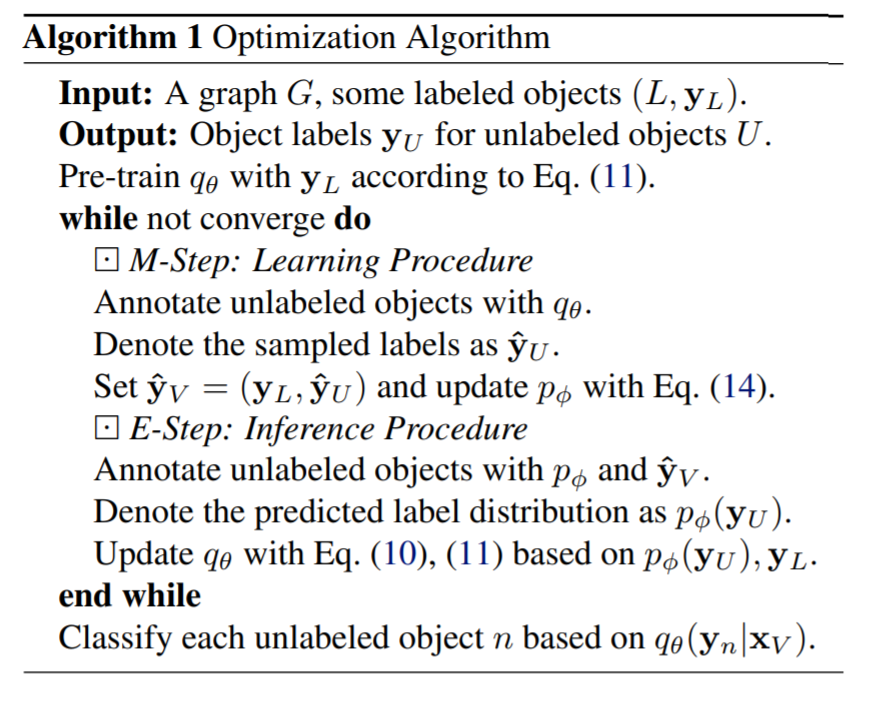
\includegraphics{gmnn-alg.PNG}
    \end{figure}
    在有标签数据上预训练$q_\theta$,再EM. 最后用$q_\theta$来预测(往往比用$p_\phi$准确率高)

\section{ClusterGCN: Fast Deep \& Large GCNs}
    \begin{figure}[htb!]
        \footnotesize
        \begin{center}
            $$
            \begin{array}{c|c|c|c|c|c|c} 
            & \text { GCN [9] } & \text { Vanilla SGD } & \text { GraphSAGE [5] } & \text { FastGCN [1] } & \text { VR-GCN [2] } & \text { Cluster-GCN } \\
            \hline \text { Time complexity } & O\left(L\|A\|_{0} F+L N F^{2}\right) & O\left(d^{L} N F^{2}\right) & O\left(r^{L} N F^{2}\right) & O\left(r L N F^{2}\right) & O\left(L\|A\|_{0} F+L N F^{2}+r^{L} N F^{2}\right) & O\left(L\|A\|_{0} F+L N F^{2}\right) \\
            \text { Memory complexity } & O\left(L N F+L F^{2}\right) & O\left(b d^{L} F+L F^{2}\right) & O\left(b r^{L} F+L F^{2}\right) & O\left(b r L F+L F^{2}\right) & O\left(L N F+L F^{2}\right) & O\left(b L F+L F^{2}\right)
            \end{array}
            $$
        \end{center}
    \end{figure}
\subsection{Vanilla ClusterGCN: Cluster For Batch}
    GCN需要整个epoch来更新一次梯度, 使用mini-batch SGD可能可以增加性能, 为此使用batch-estimator
    \begin{equation}
        \frac{1}{|\mathcal{B}|} \sum_{i \in \mathcal{B}} \nabla \operatorname{loss}\left(y_{i}, z_{i}^{(L)}\right)
    \end{equation}
    估计loss. 但这会增加一整个epoch的计算时间, SGD导致了node-repr. 聚合了$O(d^L)$个邻居的信息, 导致BP复杂度很高. 为此定义embedding utilization(嵌入效用), 为一个节点的表示在BP中被重复利用的次数. 在GCN中很高, 每层都为$d$, 但是在GraphSAGE/FastGCN中是一个很低的常数,由于k-hops很难重叠.

    为此, 考虑到一个batch的emb. util. 是其中的边数$\left\|A_{\mathcal{B}, \mathcal{B}}\right\|_{0}$, 故提出想法:每次取出边数最大的(导出)子图. 对于一个图$G$, 有分割
    \begin{equation}
        \bar{G}=\left[G_{1}, \cdots, G_{c}\right]=\left[\left\{\mathcal{V}_{1}, \mathcal{E}_{1}\right\}, \cdots,\left\{\mathcal{V}_{c}, \mathcal{E}_{c}\right\}\right]
    \end{equation}
    据此, 有
    \begin{equation}
        A=\bar{A}+\Delta=\left[\begin{array}{ccc}
        A_{11} & \cdots & A_{1 c} \\
        \vdots & \ddots & \vdots \\
        A_{c 1} & \cdots & A_{c c}
        \end{array}\right]
    \end{equation}
    以及
    \begin{equation}
        \bar{A}=\left[\begin{array}{ccc}
        A_{11} & \cdots & 0 \\
        \vdots & \ddots & \vdots \\
        0 & \cdots & A_{c c}
        \end{array}\right], \Delta=\left[\begin{array}{ccc}
        0 & \cdots & A_{1 c} \\
        \vdots & \ddots & \vdots \\
        A_{c 1} & \cdots & 0
        \end{array}\right]
    \end{equation}
    令$\bar{A}'$是正则化后的邻接矩阵, FP公式变得对于cluster分离
    \begin{equation}
        \begin{aligned}
        Z^{(L)} &=\bar{A}^{\prime} \sigma\left(\bar{A}^{\prime} \sigma\left(\cdots \sigma\left(\bar{A}^{\prime} X W^{(0)}\right) W^{(1)}\right) \cdots\right) W^{(L-1)} \\
        &=\left[\begin{array}{l}
        \bar{A}_{11}^{\prime} \sigma\left(\bar{A}_{11}^{\prime} \sigma\left(\cdots \sigma\left(\bar{A}_{11}^{\prime} X_{1} W^{(0)}\right) W^{(1)}\right) \cdots\right) W^{(L-1)} \\
        \vdots \\
        \bar{A}_{c c}^{\prime} \sigma\left(\bar{A}_{c c}^{\prime} \sigma\left(\cdots \sigma\left(\bar{A}_{c c}^{\prime} X_{c} W^{(0)}\right) W^{(1)}\right) \cdots\right) W^{(L-1)}
        \end{array}\right]
        \end{aligned}
    \end{equation}
    loss同理
    \begin{equation}
        \mathcal{L}_{\tilde{A}^{\prime}}=\sum_{t} \frac{\left|V_{t}\right|}{N} \mathcal{L}_{\tilde{A}_{t t}^{\prime}}, \mathcal{L}_{\bar{A}_{t t}^{\prime}}=\frac{1}{\left|\mathcal{V}_{t}\right|} \sum_{i \in \mathcal{V}_{t}} \operatorname{loss}\left(y_{i}, z_{i}^{(L)}\right)
    \end{equation}
    使用图节点聚类方法来产生分割(Metis or Graclus), 本作中使用的是METIS算法\footnote{
        \begin{flushleft}
            (from \href{https://en.wikipedia.org/wiki/METIS}{\bt{Wikipedia}})\bt{METIS} is a software package for graph partitioning that implements various multilevel algorithms. METIS' multilevel approach has three phases and comes with several algorithms for each phase:
        
            \begin{enumerate}
                \item Coarsen the graph by generating a sequence of graphs G0, G1, ..., GN, where G0 is the original graph and for each $0 \le i \le j \le N$, the number of vertices in Gi is greater than the number of vertices in Gj.
                \item Compute a partition of GN
                \item Project the partition back through the sequence in the order of GN, ..., G0, refining it with respect to each graph.
            \end{enumerate}
            
            The final partition computed during the third phase (the refined partition projected onto G0) is a partition of the original graph.
        \end{flushleft}
    }
\subsection{Stochastic Multiple Partitions}

    以上分割算法的问题: 固定地排除了一些边; 并且倾向于把相似的结点放在一起,可能引入bias. 解决方案: 先分割出相对大量的聚类, 再随机选取一些聚类并在一起作为batch. 加快收敛.

    \centerimage{0.85}{clustergcn-alg.png}

\subsection{Analysis of Deeper Networks}

    一个方法是增加residual-links
    \begin{equation}
        X^{(l+1)}=\sigma\left(A^{\prime} X^{(l)} W^{(l)}\right)+X^{(l)}
    \end{equation}
    另一个想法是
    \begin{equation}
        X^{(l+1)}=\sigma\left(\left(A^{\prime}+I\right) X^{(l)} W^{(l)}\right)
    \end{equation}
    用于强调上一层的embedding, 为了提供数值稳定性, 使用度正则化(区分于GCN的对称正则化)
    \begin{equation}
        \tilde{A}=(D+I)^{-1}(A+I)
    \end{equation}
    以及FP公式
    \begin{equation}
        X^{(l+1)}=\sigma\left((\tilde{A}+\lambda \operatorname{diag}(\tilde{A})) X^{(l)} W^{(l)}\right)
    \end{equation}
    实验证明这提高了深层网络的性能.

\section{GAT: Graph Attention Network}

    \begin{flushleft}
        GAT层:
        \begin{enumerate}
            \item feat. trans. $\bs h'=\bs W\bs h$
            \item atten. coeff. $e_{ij}=a(\bs h'_i, \bs h'_j)$
            \item atten. on neighbors $\bm \alpha_i = \operatorname{softmax}(\bm e_i), \alpha_{ij}=\frac{\exp \left(e_{i j}\right)}{\sum_{k \in \mathcal{N}_{i}} \exp \left(e_{i k}\right)}$, 本文中使用单层MLP+concat feat.作为注意力层, 则有
            \begin{equation}
                \alpha_{i j}=\frac{\exp \left(\text { LeakyReLU }\left(\overrightarrow{\mathbf{a}}^{T}\left[\mathbf{W} \vec{h}_{i} \| \mathbf{W} \vec{h}_{j}\right]\right)\right)}{\sum_{k \in \mathcal{N}_{i}} \exp \left(\text { Leaky } \operatorname{ReLU}\left(\overrightarrow{\mathbf{a}}^{T}\left[\mathbf{W} \vec{h}_{i} \| \mathbf{W} \vec{h}_{k}\right]\right)\right)}
            \end{equation}
            \item 进一步, 使用multi-head atten. 
            \begin{equation}
                \vec{h}_{i}^{\prime}=\|_{k=1}^{K} \sigma\left(\sum_{j \in \mathcal{N}_{i}} \alpha_{i j}^{k} \mathbf{W}^{k} \vec{h}_{j}\right)
            \end{equation}
            最终层则使用mean-aggr而非concat
            \begin{equation}
                \vec{h}_{i}^{\prime}=\sigma\left(\frac{1}{K} \sum_{k=1}^{K} \sum_{j \in \mathcal{N}_{i}} \alpha_{i j}^{k} \mathbf{W}^{k} \vec{h}_{j}\right)
            \end{equation}
            \item trick: transductive task上使用随机采样的固定大小的邻域结点
        \end{enumerate}
    \end{flushleft}

\section{Note on Probalistic Graphical Models}

\subsection{Bayesian Networks}

\begin{flushleft}
    \bt{Theorem} (d-分离的完备性)几乎所有(在测度意义上)的能被BN表征的概率分布P(CSDs)都满足: 若两节点d-分离,则它们条件独立.

    \bt{Theorem} (I-等价判定)若两个BN有相同的骨架(无向图基底)和相同的v-结构($X\to Z\leftarrow Y$)
    
    朴素贝叶斯, 贝叶斯网络(一个DAG)
\end{flushleft}

\subsection{Undirected Networks}

\begin{flushleft}
    \bt{Definition} 一个(或一些)r.v. $D$的因子是一个函数$\phi: \operatorname{dom}(D)\to \R$. 并且定义因子的乘积, $\phi_1: \operatorname{dom}((X_i)\cup (Y_j))\to \R, \phi_2: \operatorname{dom}((Y_j)\cup (Z_k))\to \R$, $\psi(\bs X, \bs Y, \bs Z) = \phi_2(\bs X, \bs Y)\times \phi_2(\bs Y, \bs Z)$.

    \bt{Definition} 一个被$$\Phi=\left\{\phi_{1}\left(\boldsymbol{D}_{1}\right), \ldots, \phi_{K}\left(\boldsymbol{D}_{K}\right)\right\}$$参数化的Gibbs分布$P_\Phi$满足
    \begin{equation}
        P_{\Phi}\left(X_{1}, \ldots, X_{n}\right)=\frac{1}{Z} \tilde{P}_{\Phi}\left(X_{1}, \ldots, X_{n}\right)
    \end{equation}
    且
    \begin{equation}
        \tilde{P}_{\Phi}\left(X_{1}, \ldots, X_{n}\right)=\phi_{1}\left(\boldsymbol{D}_{1}\right) \times \phi_{2}\left(\boldsymbol{D}_{2}\right) \times \cdots \times \phi_{m}\left(\boldsymbol{D}_{m}\right)
    \end{equation}
    其中配分函数
    \begin{equation}
        Z=\sum_{X_{1}, \ldots, X_{n}} \tilde{P}_{\Phi}\left(X_{1}, \ldots, X_{n}\right)
    \end{equation}

    \bt{Definition} MN的约化(reduction) $\cal H[\bs u]$和 $P_\Phi[\bs u]$ 定义为在变量集合$\bs U$上取值后的分布/图. 且他们是一一对应的.

    \bt{Definition} $\bs X, \bs Y$关于$\bs Z$分离, 若前二者之间没有不通过$\bs Z$的路径.

    \bt{Theorem} $P$是Gibbs分布, factorize MN$\cal H$, 则后者是前者的I-map(即独立关系包含前者).

    \bt{Theorem} (Hammersley-Clifford)$\cal H$是MN, 是前者结点上的正分布$P$的I-map, 则$P$是Gibbs分布, 且factorize MN$\cal H$.

    \bt{Theorem} 若$\bs X, \bs Y$关于$\bs Z$不分离, 那么$\bs X, \bs Y$关于$\bs Z$不独立.

    类似的,我们可以说在几乎所有分布上独立可以推出在图上分离.
    
    \bt{Definition} \begin{equation}
        \mathcal{I}_{p}(\mathcal{H})=\{(X \perp Y \mid \mathcal{X}-\{X, Y\}): X-Y \notin \mathcal{H}\}
    \end{equation}是pairwise-sepration of $\cal H$, 
    \begin{equation}
        \mathcal{I}_{\ell}(\mathcal{H})=\left\{\left(X \perp \mathcal{X}-\{X\}-\operatorname{MB}_{\mathcal{H}}(X) \mid \operatorname{MB}_{\mathcal{H}}(X)\right): X \in \mathcal{X}\right\}
    \end{equation}
    是markov-blanket of $\cal H$.

    \bt{Theorem} 以下结论等价
    l. $P \models \mathcal{I}_{\ell}(\mathcal{H})$.
    2. $P \models \mathcal{I}_{p}(\mathcal{H})$.
    3. $P \models \mathcal{I}(\mathcal{H})$.

    \bt{Definition} $\phi(\boldsymbol{D})=\exp (-\epsilon(\boldsymbol{D}))$, $\epsilon(\boldsymbol{D})$是能量函数.

    \begin{definition}
        一个分布 $P$ 是一个log-linear模型,在$\mathcal{H}$上,若它和以下参数关联:\\
            1. a set of features $\mathcal{F}=\left\{f_{1}\left(\boldsymbol{D}_{1}\right), \ldots, f_{k}\left(\boldsymbol{D}_{k}\right)\right\},$ where each $\boldsymbol{D}_{i}$ is a complete subgraph in $\mathcal{H}$,\\
            2. a set of weights $w_{1}, \ldots, w_{k}$
            such that
            $$
            P\left(X_{1}, \ldots, X_{n}\right)=\frac{1}{Z} \exp \left[-\sum_{i=1}^{k} w_{i} f_{i}\left(\boldsymbol{D}_{i}\right)\right]
            $$
    \end{definition}

    \begin{example}
        \begin{itemize}
            \item Ising Model: 二元r.v. $X_i\in\{-1, +1\}$, $\epsilon_{i, j}\left(x_{i}, x_{j}\right)=w_{i, j} x_{i} x_{j}$, 有能量函数\begin{equation}
                P(\xi)=\frac{1}{Z} \exp \left(-\sum_{i<j} w_{i, j} x_{i} x_{j}-\sum_{i} u_{i} x_{i}\right)
            \end{equation}
            \item Boltzmann Dist.: 二元r.v. $X_i\in\{0, 1\}$, 边上的能量如同Ising模型, 但每个随机变量都分配了pdf $\operatorname{sigmoid}(z),z=-\left(\sum_{j} w_{i, j} x_{j}\right)-w_{i}$
            \item Metric CRF:使用CRF来标注图节点, 有能量函数\begin{equation}
                E\left(x_{1}, \ldots, x_{n}\right)=\sum_{i} \epsilon_{i}\left(x_{i}\right)+\sum_{(i, j) \in \mathcal{E}} \epsilon_{i, j}\left(x_{i}, x_{j}\right)
            \end{equation}
            其中能量函数的取法导致了不同的模型, Ising Model:
            \begin{equation}
                \epsilon_{i, j}\left(x_{i}, x_{j}\right)=\left\{\begin{array}{ll}
                0 & x_{i}=x_{j} \\
                \lambda_{i, j} & x_{i} \neq x_{j}
                \end{array}\right.=\delta_{x_i, x_j}\lambda_{i, j}
            \end{equation}
            Potts Model定义了结点的度规函数$\mu$(需要满足非负性, 自反性, 三角不等式)用于能量函数, 并适用于多种标签的情况. 若一个度规满足前二者(非负性, 自反性), 则称其为semi-metric/半度规的. CV中常用的能量函数截断范数
            \begin{equation}
                \epsilon\left(x_{i}, x_{j}\right)=\min \left(c\left\|x_{i}-x_{j}\right\|_{p}, \operatorname{dist}_{\max }\right)
            \end{equation}
        \end{itemize}
    \end{example}

    \begin{definition}
        令$\ell (\xi)=\log P(\xi)$Canonical energy on clique, 关于一个特定的赋值$\xi^{*}=\left(x_{1}^{*}, \ldots, x_{n}^{*}\right)$
        \begin{equation}
            \epsilon_{\bs D}^{*}(\boldsymbol{d})=\sum_{Z \subset D}(-1)^{|D-Z|} \ell\left(\boldsymbol{d}_{\boldsymbol{Z}}, \xi_{-\boldsymbol{Z}}^{*}\right)
        \end{equation}
    \end{definition}

    \begin{proposition}
        Let $\mathcal{B}$ be a Bayesian network over $\mathcal{X}$ and $\boldsymbol{E}=\boldsymbol{e}$ an obseruation. Let $\boldsymbol{W}=\mathcal{X}-\boldsymbol{E}$. Then $P_{\mathcal{B}}(\boldsymbol{W} \mid \boldsymbol{e})$ is a Gibbs distribution defined by the factors $\Phi=\left\{\phi_{X_{i}}\right\}_{\mathcal{X}_{i} \in \mathcal{X}},$ where
        $$
        \phi_{X_{i}}=P_{\mathcal{B}}\left(X_{i} \mid \mathrm{Pa}_{X_{i}}\right)[\boldsymbol{E}=\boldsymbol{e}]
        $$
        The partition function for this Gibbs distribution is $P(e)$
    \end{proposition}

    \begin{definition}
        Moralized map for BN$\cal G$定义为一个同样节点的无向图$M[\cal G]$, 其中一条边$(X,Y)$存在若在$\cal G$中有一条有向边连接, 或者他们是moral的(具有相同的子结点).
    \end{definition}

    \begin{proposition}
        For BN $\cal G$, $M[\cal G]$是极小I-map.
    \end{proposition}

    \begin{proposition}
        Let $\boldsymbol{X}, \boldsymbol{Y}, \boldsymbol{Z}$ be three disjoint sets of nodes in a Bayesian network $\mathcal{G} .$ Let $\boldsymbol{U}=\boldsymbol{X} \cup \boldsymbol{Y} \cup \boldsymbol{Z},$ and
        let $\mathcal{G}^{\prime}=\mathcal{G}^{+}[\boldsymbol{U}]$ be the induced Bayesian network over $\boldsymbol{U} \cup$ Ancestors $_{U}$. Let $\mathcal{H}$ be the moralized $\operatorname{graph} \mathcal{M}\left[\mathcal{G}^{\prime}\right] .$ Then $\mathrm{d}-\operatorname{sep}_{\mathcal{G}}(\boldsymbol{X} ; \boldsymbol{Y} \mid \boldsymbol{Z})$ if and only if $\operatorname{sep}_{\mathcal{H}}(\boldsymbol{X} ; \boldsymbol{Y} \mid \boldsymbol{Z})$
    \end{proposition}

    \begin{theorem}
        若MN $\cal H$是弦图, 则存在BN $\mathcal{G}$ such that $\mathcal{I}(\mathcal{H})=\mathcal{I}(\mathcal{G})$
    \end{theorem}

    \begin{figure}[htb!]
        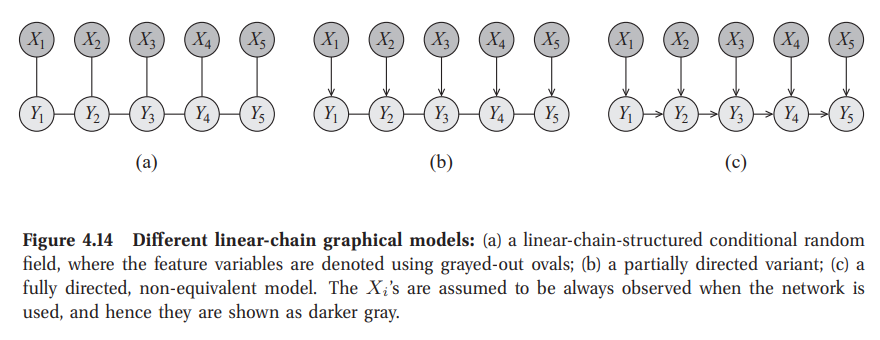
\includegraphics{pgm-1.PNG}
    \end{figure}

    \begin{definition}
        CRF 是一个无向图$\cal H$, 节点为$\bs X\cup \bs Y$, 带有因子$\phi_{1}\left(\boldsymbol{D}_{1}\right), \ldots, \phi_{m}\left(\boldsymbol{D}_{m}\right) \text { such that each } \boldsymbol{D}_{i} \nsubseteq \boldsymbol{X}$, models dist. such as 
        \begin{equation}
            \begin{aligned}
            P(\boldsymbol{Y} \mid \boldsymbol{X}) &=\frac{1}{Z(\boldsymbol{X})} \tilde{P}(\boldsymbol{Y}, \boldsymbol{X}) \\
            \tilde{P}(\boldsymbol{Y}, \boldsymbol{X}) &=\prod_{i=1}^{m} \phi_{i}\left(\boldsymbol{D}_{i}\right) \\
            Z(\boldsymbol{X}) &=\sum_{Y} \tilde{P}(\boldsymbol{Y}, \boldsymbol{X})
            \end{aligned}
        \end{equation}
    \end{definition}

    \begin{example}
        考虑只有一个$Y$的CRF(朴素Markov模型),能量函数
        \begin{equation}
            \phi_{i}\left(X_{i}, Y\right)=\exp \left\{w_{i} \boldsymbol{I}\left\{X_{i}=1, Y=1\right\}\right\}
        \end{equation}
        我们可以得到
        \begin{equation}
            P\left(Y=1 \mid x_{1}, \ldots, x_{k}\right)=\operatorname{sigmoid}\left(w_{0}+\sum_{i=1}^{k} w_{i} x_{i}\right)
        \end{equation}
        a sigmoid-regression model! 
    \end{example}
\end{flushleft}

\subsection{Local Probablistic Models | i.e. Specific Models Corresponds to Last 2 Sections}
\begin{flushleft}
    表式\trarr 复杂度极高!

    确定性CPD由父节点的函数决定
    \begin{equation}
        P\left(x \mid \mathrm{pa}_{X}\right)=\left\{\begin{array}{ll}
        1 & x=f\left(\mathrm{pa}_{X}\right) \\
        0 & \text { otherwise }
        \end{array}\right.
    \end{equation}

    树形CPD: 类似于决策树, 但每个节点都annotate一个子结点上的分布

    基于规则的CPD

    noisy-or CPD 
    \begin{equation}
        \begin{aligned}
        P\left(y^{0} \mid X_{1}, \ldots, X_{k}\right) &=\left(1-\lambda_{0}\right) \prod_{i: X_{i}=x_{i}^{1}}\left(1-\lambda_{i}\right) \\
        P\left(y^{1} \mid X_{1}, \ldots, X_{k}\right) &=1-\left[\left(1-\lambda_{0}\right) \prod_{i: X_{i}=x_{i}^{1}}\left(1-\lambda_{i}\right)\right]
        \end{aligned}
    \end{equation}

    sigmoid CPD
    \begin{equation}
        P\left(y^{1} \mid X_{1}, \ldots, X_{k}\right)=\operatorname{sigmoid}\left(w_{0}+\sum_{i=1}^{k} w_{i} X_{i}\right)
    \end{equation}

    Gaussian CPD 
    \begin{equation}
        p\left(Y \mid x_{1}, \ldots, x_{k}\right)=\mathcal{N}\left(\beta_{0}+\beta_{1} x_{1}+\cdots+\beta_{k} x_{k} ; \sigma^{2}\right)
    \end{equation}
    写成向量, 则为
    \begin{equation}
        p(Y \mid \boldsymbol{x})=\mathcal{N}\left(\beta_{0}+\boldsymbol{\beta}^{T} \boldsymbol{x} ; \sigma^{2}\right)
    \end{equation}

    条件线性高斯模型(CLG)
    \begin{equation}
        p(X \mid \boldsymbol{u}, \boldsymbol{y})=\mathcal{N}\left(a_{\boldsymbol{u}, 0}+\sum_{i=1}^{k} a_{\boldsymbol{u}, i} y_{i} ; \sigma_{\boldsymbol{u}}^{2}\right)
    \end{equation}

    \begin{definition}
        (conditional Bayesian networks) 条件贝叶斯网络$\cal G$是一个DAG, 节点是分离的三个集合的并 $\boldsymbol{X} \cup \boldsymbol{Y} \cup \boldsymbol{Z}$, $\bs X$没有父节点, 称作输入, $\bs Y$称作输出, 且条件概率分布由链式法则定义
        \begin{equation}
            P_{\mathcal{B}}(\boldsymbol{Y}, \boldsymbol{Z} \mid \boldsymbol{X})=\prod_{X \in Y \cup Z} P\left(X \mid \mathrm{Pa}_{X}^{\mathcal{G}}\right)
        \end{equation}.
        边缘分布由求和给出
        \begin{equation}
            P_{\mathcal{B}}(\boldsymbol{Y} \mid \boldsymbol{X})=\sum_{\boldsymbol{Z}} P_{\mathcal{B}}(\boldsymbol{Y}, \boldsymbol{Z} \mid \boldsymbol{X})
        \end{equation}
        
    \end{definition}

\end{flushleft}

\subsection{Temporal Models}
\begin{flushleft}
    
\end{flushleft}

\section{RSCNN(CVPR 19')}
\begin{figure}
    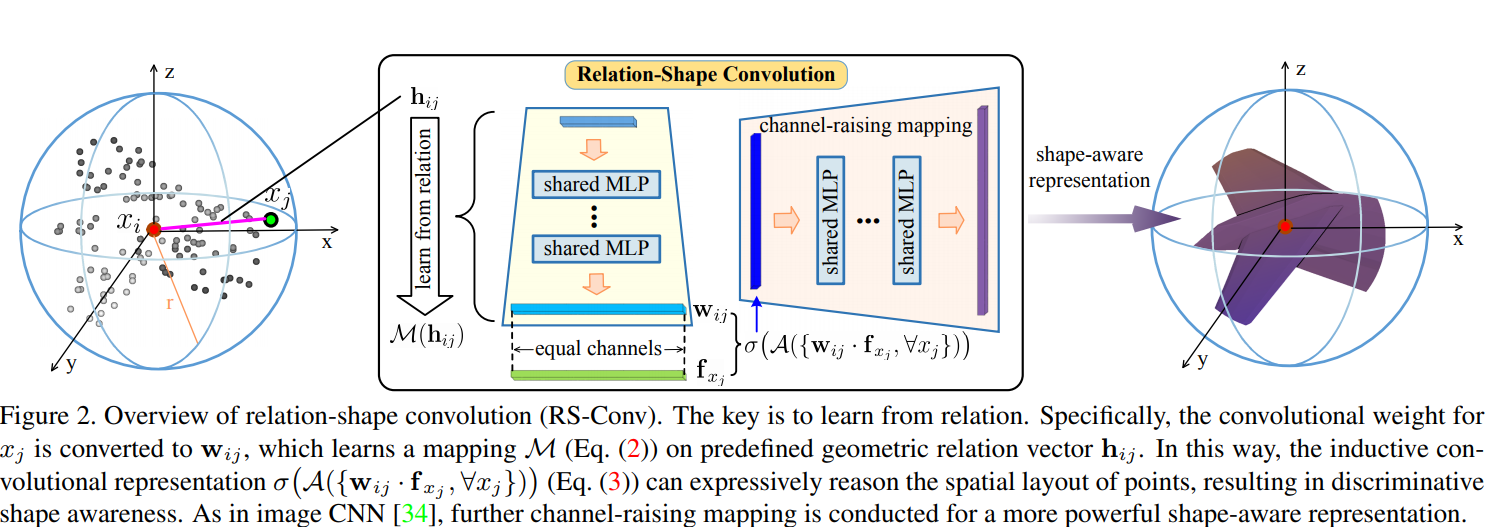
\includegraphics[width=0.85\paperwidth]{rscnn-arch.PNG}
\end{figure}
\subsection{Architecture}
\begin{flushleft}
    \begin{idea}
        使用空间卷积/spatial conv., 在球形邻域上.
    \end{idea}

    一个广义卷积
    \begin{equation}
        \mathbf{f}_{P_{\text {sub }}}=\sigma\left(\mathcal{A}\left(\left\{\mathcal{T}\left(\mathbf{f}_{x_{j}}\right), \forall x_{j}\right\}\right)\right), d_{i j}<r \forall x_{j} \in \mathcal{N}\left(x_{i}\right)
    \end{equation}
    要想是这个卷积permut.-invar., 函数$\cal{A, T}$必须分别是对称的和shared.

    使用shape-awared/geometric info 函数$\cal M$(shared MLP建模)代替传统卷积
    \begin{equation}
        \mathcal{T}\left(\mathbf{f}_{x_{j}}\right)=\mathbf{w}_{i j} \cdot \mathbf{f}_{x_{j}}=\mathcal{M}\left(\mathbf{h}_{i j}\right) \cdot \mathbf{f}_{x_{j}}
    \end{equation}
    则卷积形式变为
    \begin{equation}
        \mathbf{f}_{P_{\text {sub }}}=\sigma\left(\mathcal{A}\left(\left\{\mathcal{M}\left(\mathbf{h}_{i j}\right) \cdot \mathbf{f}_{x_{j}}, \forall x_{j}\right\}\right)\right)
    \end{equation}

    为了和CNN相对应, 使用channel-raising MLP来增多channels.

    最终, 这个卷积具有以下性质: permut. invar., 对于刚性变换的健壮性, shared weights, interacted point geometric.
\end{flushleft}
\subsection{Details \& Implementation}
\begin{flushleft}
    使用ReLU激活函数, 使用BN, $\cal M$使用三层MLP, aggr. f. 为max-pooling. Low-level几何表示$\bs h_{ij}=[\bs x_i-\bs x_j, \bs x_i, \bs x_j]$, channel-raising使用单层MLP.

    点云采样方面, 使用原点云的FPS采样. 使用3-scale邻域(不同于PN++的MSG)
\end{flushleft}
\section{SimpleView(ICLR 21' Candidate)}

\subsection{Simple Review of Existing Protocols}

\begin{flushleft}
    \bt{数据增强}: 包括抖动, y-轴随机旋转, 随即平移和缩放. ModelNet40由于已经对齐, y-轴随机旋转会降低性能.
    \begin{tabular}{|c|c|c|c|}
        Model & PointNet(++) & DGCNN & RSCNN \\
        \hline
            & All & 随机旋转/平移 & 随机旋转/平移
    \end{tabular}

    \bt{输入点数} PN(++)使用1024个固定输入. PointCNN, RSCNN使用每个epoch重采样的点.

    \bt{Loss} 大多数方法使用交叉熵, DGCNN使用了平滑了的交叉熵(label经过平滑, 这个方法在所有结构上提高了性能)

    \bt{模型选择} PN(++)使用最终收敛的模型, DGCNN/RSCNN使用测试集上的最好模型.

    \bt{模型聚合} PN(++)在inference-time把最终模型在不同旋转角度的输入上做判定(10次), 然后投票决定. RSCNN, DensePoint在不同尺寸和角度的输入上判定(300次), 然后投票决定. DGCNN完全没有投票.

    比较性能, 本文提出的方法使用随机平移/缩放强化和smooth-loss, 并且为了不利用任何测试集的信息, 使用final model sel.
\end{flushleft}

\subsection{Model: SimpleView}

\begin{flushleft}
    \begin{idea}
        使用多个视角的深度图像!
    \end{idea}

    具体上, 使用六个view(水平面四个, z轴两个, 实验上这样性能最好), 并且在每张深度图上使用ResNet18/4骨架(ResNet18, 滤波器数量为1/4), concat连接特征.
\end{flushleft}

\section{OT-Flow}

\subsection{Idea \& Formulations}

\begin{flushleft}
    Formulation(based on FFJORD)
    \begin{equation}
        \partial_{t}\left[\begin{array}{c}
        \boldsymbol{z}(\boldsymbol{x}, t) \\
        \ell(\boldsymbol{x}, t)
        \end{array}\right]=\left[\begin{array}{c}
        \mathbf{v}(\boldsymbol{z}(\boldsymbol{x}, t), t ; \boldsymbol{\theta}) \\
        \operatorname{tr}(\nabla \mathbf{v}(\boldsymbol{z}(\boldsymbol{x}, t), t ; \boldsymbol{\theta}))
        \end{array}\right], \quad\left[\begin{array}{l}
        \boldsymbol{z}(\boldsymbol{x}, 0) \\
        \ell(\boldsymbol{x}, 0)
        \end{array}\right]=\left[\begin{array}{l}
        \boldsymbol{x} \\
        0
        \end{array}\right]
    \end{equation}

    在FFJORD的基础
    \begin{equation}
        \min _{\boldsymbol{\theta}} \mathbb{E}_{\rho_{0}(\boldsymbol{x})}\left\{C(\boldsymbol{x}, T):=\frac{1}{2}\|\boldsymbol{z}(\boldsymbol{x}, T)\|^{2}-\ell(\boldsymbol{x}, T)+\frac{d}{2} \log (2 \pi)\right\}
    \end{equation}
    上增加最优输运代价
    \begin{equation}
        L(\boldsymbol{x}, T)=\int_{0}^{T} \frac{1}{2}\|\mathbf{v}(\boldsymbol{z}(\boldsymbol{x}, t), t)\|^{2} \mathrm{d} t
    \end{equation}
    满足上两个cost的和最小化时, 则必定存在势函数
    \begin{equation}
        \mathbf{v}(\boldsymbol{x}, t ; \boldsymbol{\theta})=-\nabla \Phi(\boldsymbol{x}, t ; \boldsymbol{\theta})
    \end{equation}
    并且满足HJB方程(Hamilton-Jacobi-Bellman Eq.)
    \begin{equation}
        -\partial_{t} \Phi(\boldsymbol{x}, t)+\frac{1}{2}\|\nabla \Phi(\boldsymbol{z}(\boldsymbol{x}, t), t)\|^{2}=0, \quad \Phi(\boldsymbol{x}, T)=G(\boldsymbol{x})
    \end{equation}
    故引入惩罚项
    \begin{equation}
        R(\boldsymbol{x}, T)=\int_{0}^{T}\left|\partial_{t} \Phi(\boldsymbol{z}(\boldsymbol{x}, t), t)-\frac{1}{2}\|\nabla \Phi(\boldsymbol{z}(\boldsymbol{x}, t), t)\|^{2}\right| \mathrm{d} t
    \end{equation}
    本工作直接不建模梯度函数$\bs v$, 而是直接建模势函数$\Phi$.

\end{flushleft}

\subsection{Parametrization of Model}

\begin{flushleft}
    势函数
    \begin{equation}
        \Phi(\boldsymbol{s} ; \boldsymbol{\theta})=\boldsymbol{w}^{\top} N\left(\boldsymbol{s} ; \boldsymbol{\theta}_{N}\right)+\frac{1}{2} \boldsymbol{s}^{\top}\left(\boldsymbol{A}^{\top} \boldsymbol{A}\right) \boldsymbol{s}+\boldsymbol{b}^{\top} \boldsymbol{s}+c, \quad \text { where } \boldsymbol{\theta}=\left(\boldsymbol{w}, \boldsymbol{\theta}_{N}, \boldsymbol{A}, \boldsymbol{b}, c\right)
    \end{equation}
    其中$N$是一个NN(这里用的是一个简单的两层ResNet), $\boldsymbol{A} \in \mathbb{R}^{r \times(d+1)}$, 且限制rank $r=\max(10, d)$
    这里后面三项建模了一个二次势函数, 也即一个线性动力系统, NN则建模了非线性部分.

    ResNet结构
    \begin{equation}
        \begin{aligned}
        \boldsymbol{u}_{0} &=\sigma\left(\boldsymbol{K}_{0} \boldsymbol{s}+\boldsymbol{b}_{0}\right) \\
        N\left(\boldsymbol{s} ; \boldsymbol{\theta}_{N}\right)=\boldsymbol{u}_{1} &=\boldsymbol{u}_{0}+h \sigma\left(\boldsymbol{K}_{1} \boldsymbol{u}_{0}+\boldsymbol{b}_{1}\right)
        \end{aligned}
    \end{equation}

    梯度计算
    \begin{equation}
        \nabla_{s} \Phi(s ; \boldsymbol{\theta})=\nabla_{s} N\left(\boldsymbol{s} ; \boldsymbol{\theta}_{N}\right) \boldsymbol{w}+\left(\boldsymbol{A}^{\top} \boldsymbol{A}\right) \boldsymbol{s}+\boldsymbol{b}
    \end{equation}

    Hessian Trace计算
    \begin{equation}
        \operatorname{tr}\left(\nabla^{2} \Phi(\boldsymbol{s} ; \boldsymbol{\theta})\right)=\operatorname{tr}\left(\boldsymbol{E}^{\top} \nabla_{\boldsymbol{s}}^{2}\left(N\left(\boldsymbol{s} ; \boldsymbol{\theta}_{N}\right) \boldsymbol{w}\right) \boldsymbol{E}\right)+\operatorname{tr}\left(\boldsymbol{E}^{\top}\left(\boldsymbol{A}^{\top} \boldsymbol{A}\right) \boldsymbol{E}\right)
    \end{equation}
    后一项是trivial的, $\bs E$是$\R^(d+1)$标准正交基的前d项,ResNet项可以得到一个闭形式
    \begin{equation}
        \begin{aligned}
        \operatorname{tr}\left(\boldsymbol{E}^{\top} \nabla_{\boldsymbol{s}}^{2}\left(N\left(\boldsymbol{s} ; \boldsymbol{\theta}_{N}\right) \boldsymbol{w}\right) \boldsymbol{E}\right) &=t_{0}+h t_{1}, \quad \text { where } \\
        t_{0} &=\left(\sigma^{\prime \prime}\left(\boldsymbol{K}_{0} \boldsymbol{s}+\boldsymbol{b}_{0}\right) \odot \boldsymbol{z}_{1}\right)^{\top}\left(\left(\boldsymbol{K}_{0} \boldsymbol{E}\right) \odot\left(\boldsymbol{K}_{0} \boldsymbol{E}\right)\right) \boldsymbol{1} \\
        t_{1} &=\left(\sigma^{\prime \prime}\left(\boldsymbol{K}_{1} \boldsymbol{u}_{0}+\boldsymbol{b}_{1}\right) \odot \boldsymbol{w}\right)^{\top}\left(\left(\boldsymbol{K}_{1} \nabla_{\boldsymbol{s}} \boldsymbol{u}_{0}^{\top}\right) \odot\left(\boldsymbol{K}_{1} \nabla_{\boldsymbol{s}} \boldsymbol{u}_{0}^{\top}\right)\right) \mathbf{1}
        \end{aligned}
    \end{equation}
    第一层的Hessian计算复杂度$O(m d)$,之后每多一层为 $O(m^2 d)$, 总复杂度则为$O(d)$

\end{flushleft}

\subsection{Exact Hessian of Multilayer NN}
\begin{flushleft}
    Exact Trace Computation Using (13) and the same $E$, we compute the trace in one forward pass through the layers. The trace of the first ResNet layer is
$$
\begin{aligned}
t_{0} &=\operatorname{tr}\left(\boldsymbol{E}^{\top} \nabla_{\boldsymbol{s}}\left(\boldsymbol{K}_{0}^{\top} \operatorname{diag}\left(\sigma^{\prime \prime}\left(\boldsymbol{K}_{0} \boldsymbol{s}+\boldsymbol{b}_{0}\right)\right) \boldsymbol{z}_{1}\right) \boldsymbol{E}\right) \\
&=\operatorname{tr}\left(\boldsymbol{E}^{\top} \boldsymbol{K}_{0}^{\top} \operatorname{diag}\left(\sigma^{\prime \prime}\left(\boldsymbol{K}_{0} \boldsymbol{s}+\boldsymbol{b}_{0}\right) \odot \boldsymbol{z}_{1}\right) \boldsymbol{K}_{0} \boldsymbol{E}\right) \\
&=\left(\sigma^{\prime \prime}\left(\boldsymbol{K}_{0} \boldsymbol{s}+\boldsymbol{b}_{0}\right) \odot \boldsymbol{z}_{1}\right)^{\top}\left(\left(\boldsymbol{K}_{0} \boldsymbol{E}\right) \odot\left(\boldsymbol{K}_{0} \boldsymbol{E}\right)\right) \mathbf{1}
\end{aligned}
$$
using the same notation as (14). For the last step, we used the diagonality of the middle matrix. Computing $t_{0}$ requires $\mathcal{O}(m \cdot d)$ FLOPS when first squaring the elements in the first $d$ columns of $\boldsymbol{K}_{0}$, then summing those columns, and finally one inner product.

To compute the trace of the entire ResNet, we continue with the remaining rows in (27) in reverse order to obtain
$$
\operatorname{tr}\left(\boldsymbol{E}^{\top} \nabla_{\boldsymbol{s}}^{2}\left(N\left(\boldsymbol{s} ; \boldsymbol{\theta}_{N}\right) \boldsymbol{w}\right) \boldsymbol{E}\right)=t_{0}+h \sum_{i=1}^{M} t_{i}
$$
where $t_{i}$ is computed as
$$
\begin{aligned}
t_{i} &=\operatorname{tr}\left(J_{i-1}^{\top} \nabla_{\boldsymbol{s}}\left(\boldsymbol{K}_{i}^{\top} \operatorname{diag}\left(\sigma^{\prime \prime}\left(\boldsymbol{K}_{i} \boldsymbol{u}_{i-1}(\boldsymbol{s})+\boldsymbol{b}_{i}\right)\right) \boldsymbol{z}_{i+1}\right) J_{i-1}\right) \\
&=\operatorname{tr}\left(J_{i-1}^{\top} \boldsymbol{K}_{i}^{\top} \operatorname{diag}\left(\sigma^{\prime \prime}\left(\boldsymbol{K}_{i} \boldsymbol{u}_{i-1}+\boldsymbol{b}_{i}\right) \odot \boldsymbol{z}_{i+1}\right) \boldsymbol{K}_{i} J_{i-1}\right) \\
&=\left(\sigma^{\prime \prime}\left(\boldsymbol{K}_{i} \boldsymbol{u}_{i-1} \mid \boldsymbol{b}_{i}\right) \odot \boldsymbol{z}_{i+1}\right)^{\top}\left(\left(\boldsymbol{K}_{i} J_{i-1}\right) \odot\left(\boldsymbol{K}_{i} J_{i-1}\right)\right) \mathbf{1}
\end{aligned}
$$
Here, $J_{i-1}=\nabla_{s} \boldsymbol{u}_{i-1}^{\top} \in \mathbb{R}^{m \times d}$ is a Jacobian matrix, which can be updated and over-written in the forward pass at a computational cost of $\mathcal{O}\left(m^{2} \cdot d\right)$ FLOPS. The $J$ update follows:
$$
\begin{aligned}
\nabla_{\boldsymbol{s}} \boldsymbol{u}_{i}^{\top} &=\nabla_{\boldsymbol{s}} \boldsymbol{u}_{i-1}+h \sigma^{\prime}\left(\boldsymbol{K}_{i} \boldsymbol{u}_{i-1}+\boldsymbol{b}_{i}\right) \boldsymbol{K}_{i}^{\top} \nabla_{\boldsymbol{s}} \boldsymbol{u}_{i-1} \\
J & \leftarrow J+h \sigma^{\prime}\left(\boldsymbol{K}_{i} \boldsymbol{u}_{i-1}+\boldsymbol{b}_{i}\right) \boldsymbol{K}_{i}^{\top} J
\end{aligned}
$$
\end{flushleft}

\section{Node2vec: Unsupervised Feature Learning}
\begin{figure}[htbp]
    \centering
    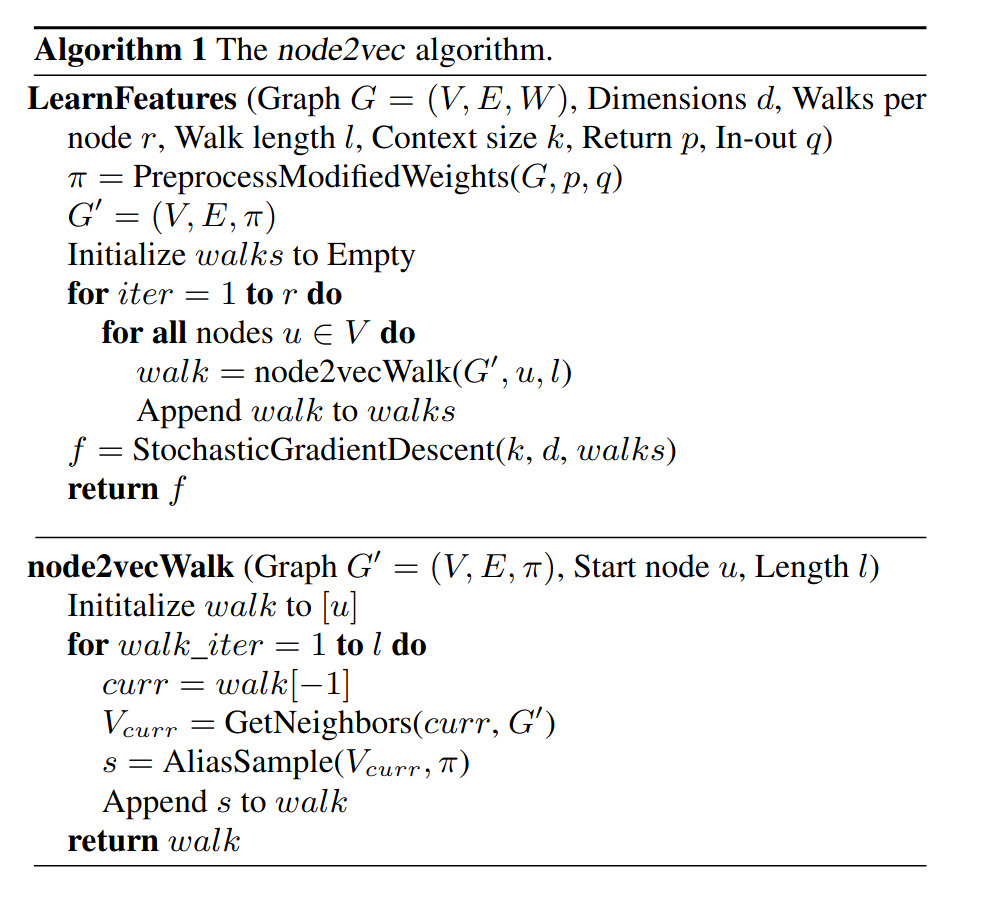
\includegraphics[width=0.7\textwidth]{node2vec-alg.png}
\end{figure}

\subsection{Basics}
\begin{flushleft}
    MF approx. + lld optimization, 在某种采样策略S下:
    \begin{equation}
        \max _{f} \sum_{u \in V} \log \operatorname{Pr}\left(N_{S}(u) \mid f(u)\right)
    \end{equation}
    进一步使用MF(邻域内条件独立)
    \begin{equation}
        \operatorname{Pr}\left(N_{S}(u) \mid f(u)\right)=\prod_{n_{i} \in N_{S}(u)} \operatorname{Pr}\left(n_{i} \mid f(u)\right)
    \end{equation}
    特征空间对称性(点之间)给出
    \begin{equation}
        \operatorname{Pr}\left(n_{i} \mid f(u)\right)=\frac{\exp \left(f\left(n_{i}\right) \cdot f(u)\right)}{\sum_{v \in V} \exp (f(v) \cdot f(u))}
    \end{equation}
    最后优化目标为
    \begin{equation}
        \max _{f} \sum_{u \in V}\left[-\log Z_{u}+\sum_{n_{i} \in N_{S}(u)} f\left(n_{i}\right) \cdot f(u)\right]
    \end{equation}
\end{flushleft}
\subsection{Biased Random Walk}
\begin{flushleft}
    不同与传统的BFS/DFS,采用一种折衷的方法(二阶Markov随机游走),设上一步为$(t\to v)$,则下一步的转移概率为$\pi_{vx}=\alpha_{pq}(t,x)$,其中
    \begin{equation}
        \alpha_{p q}(t, x)=\left\{\begin{array}{ll}
        \frac{1}{p} & \text { if } d_{t x}=0 \\
        1 & \text { if } d_{t x}=1 \\
        \frac{1}{q} & \text { if } d_{t x}=2
        \end{array}\right.
    \end{equation}
    其中$d_{uv}$是节点最短路径.

    考虑其中的参数\begin{enumerate}
        \item Return Param. $p$, 控制了回到之前的点的概率. 设为较高的值($>\max(q, 1)$)可以防止回到原点, 设为较低的值($<\max(p, 1)$)则会鼓励在原点附近探索.
        \item In-out Param. $q$. 大于1的值偏向于探索原点附近的节点,小于1的值偏向于DFS那样的远离探索.
    \end{enumerate}

    $l$长度的游走可以为$k$个节点生成$l-k$大小的邻域,总时间复杂度为$O(\frac{l}{k(l-k)})$
\end{flushleft}
\subsection{Edge Feature}
简单的在节点间使用edge feature generator即可

\begin{equation}
    \begin{array}{l|c|c}
    \text { Operator } & \text { Symbol } & \text { Definition } \\
    \hline \text { Average } & \oplus & {[f(u) \oplus f(v)]_{i}=\frac{f_{i}(u)+f_{i}(v)}{2}} \\
    \text { Hadamard } & \square & {[f(u) \square f(v)]_{i}=f_{i}(u) * f_{i}(v)} \\
    \text { Weighted-L1 } & \|\cdot\|_{\overline{1}} & \|f(u) \cdot f(v)\|_{\overline{1} i}=\left|f_{i}(u)-f_{i}(v)\right| \\
    \text { Weighted-L2 } & \|\cdot\|_{\overline{2}} & \|f(u) \cdot f(v)\|_{\overline{2} i}=\left|f_{i}(u)-f_{i}(v)\right|^{2}
    \end{array}
\end{equation}

\section{DeepWalk: Online Representation Learning}

\bt{Note} 自然语言中词语的出现pdf和社交图中节点在短随机游走中出现的概率都近似服从幂律分布.

\begin{figure}[htbp]
    \centering
    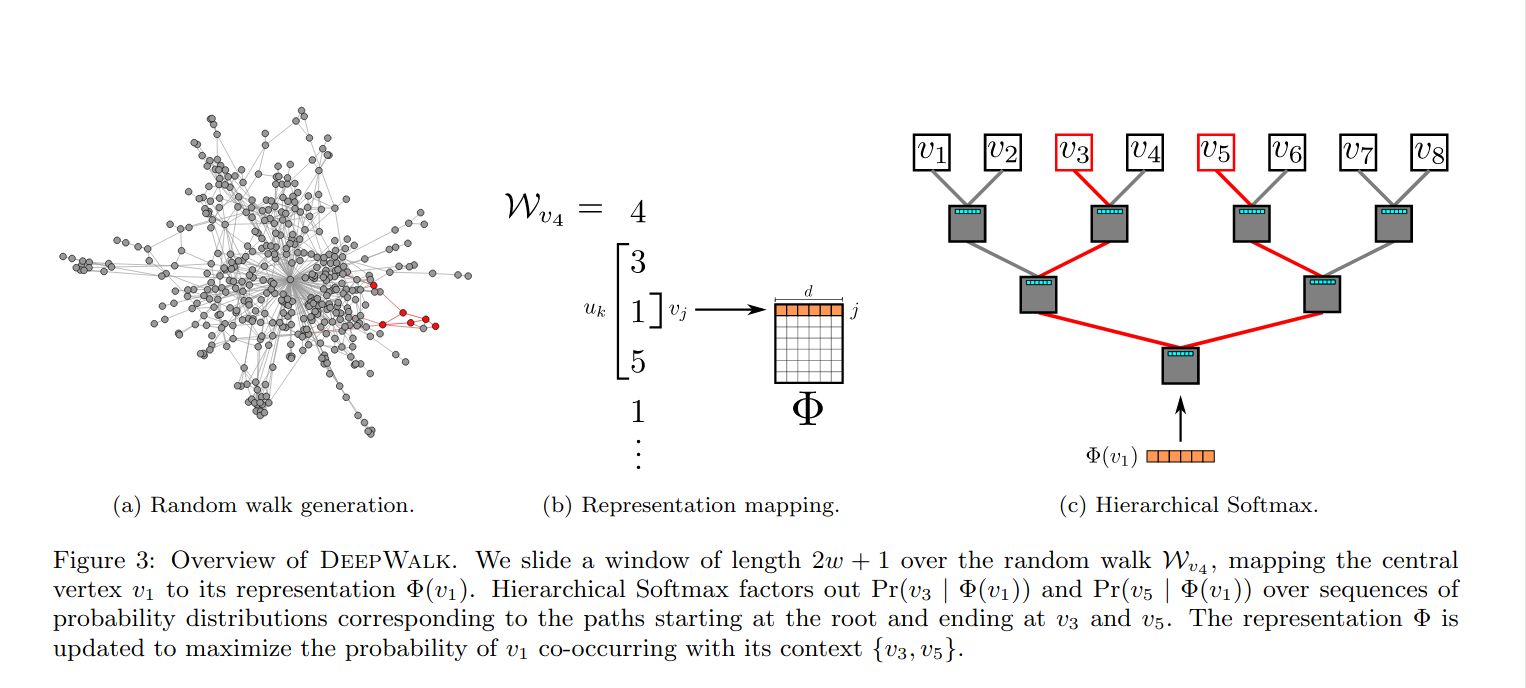
\includegraphics[width=0.95\textwidth]{deepwalk-overview.png}
\end{figure}

\subsection{DeepWalk}
\begin{figure}[htbp]
    \centering
    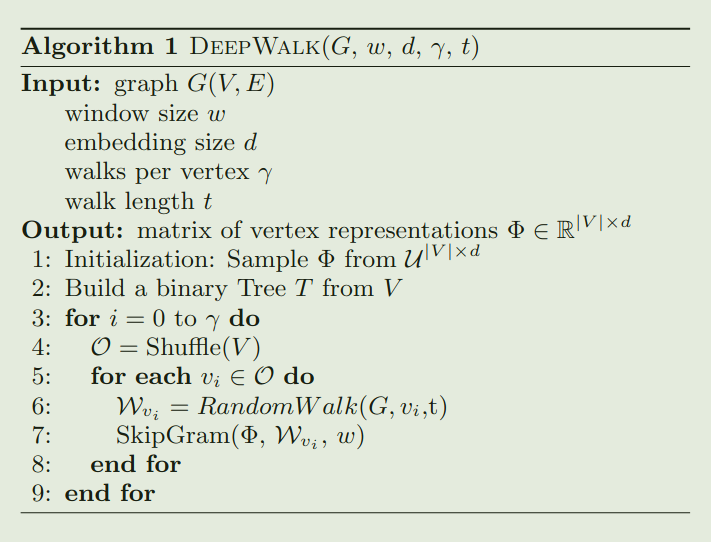
\includegraphics[width=0.7\textwidth]{deepwalk-deepwalk.png}
\end{figure}

从图中的每个节点开始(使用一个随机生成的二叉生成树来指定顺序), 进行随机游走, 长度不定, 在邻域上均匀采样决定下一个节点, 接着使用\verb|SkipGram|算法来更新节点表示. 每一个生成的随机游走为$\mathcal{W}_{v_i}$,长度为t. 注意, 特征的形式为表式$\Phi\in \R^{|V|\times d}$

\subsection{SkipGram}
\begin{figure}[htbp]
    \centering
    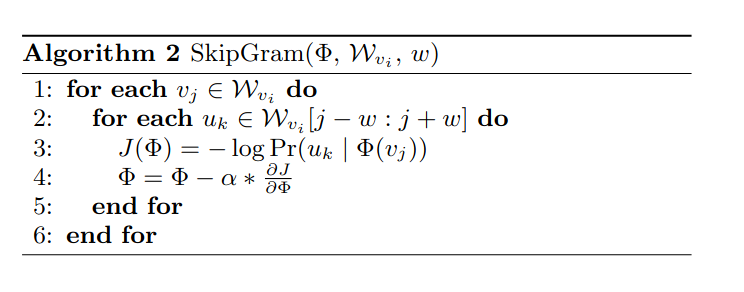
\includegraphics[width=0.7\textwidth]{deepwalk-skipgram.png}
\end{figure}

SkipGram是一个最大化一句话中词汇co-occurence概率的算法. 最大化每个窗口中的lld $J(\Phi)=-\log \operatorname{Pr}(u_k|\Phi(v_j))$. 为了方便计算lld,引入Hierachical Softmax.

\subsection{Hierachichal Softmax}

把每一个节点放到一个二叉树的树叶上, 然后每个节点的lld为按照一个从根到叶子节点的路径(的乘积)
\begin{equation}
    \operatorname{Pr}\left(u_{k} \mid \Phi\left(v_{j}\right)\right)=\prod_{l=1}^{\lceil\log |V|\rceil} \operatorname{Pr}\left(b_{l} \mid \Phi\left(v_{j}\right)\right)
\end{equation}
中间每一层都是
这样,一个节点的所有条件lld的计算代价为$O(|V|\log |V|)$
还可以通过Huffman树来让常用的节点到根的长度更小.\footnote{
    A brief supplement from NLP:
    中间节点每一项都是一个二分类器/Logistic Reg.:
    \begin{equation}
        p\left(d_{j}^{w} \mid \mathbf{x}_{w}, \theta_{j-1}^{w}\right)=\left\{\begin{array}{ll}
        \sigma\left(\mathbf{x}_{w}^{\top} \theta_{j-1}^{w}\right), & d_{j}^{w}=0 \\
        1-\sigma\left(\mathbf{x}_{w}^{\top} \theta_{j-1}^{w}\right), & d_{j}^{w}=1
        \end{array}\right.
    \end{equation}
    其中$w$是那个word/节点, $d_j^w$是中间节点/二叉树指示编码, 写成一个式子为
    \begin{equation}
        p\left(d_{j}^{w} \mid \mathbf{x}_{w}, \theta_{j-1}^{w}\right)=\left[\sigma\left(\mathbf{x}_{w}^{\top} \theta_{j-1}^{w}\right)\right]^{1-d_{j}^{w}} \cdot\left[1-\sigma\left(\mathbf{x}_{w}^{\top} \theta_{j-1}^{w}\right)\right]^{d^{w}}
    \end{equation}
    lld为
    \begin{equation}
        \begin{array}{l}
        \mathcal{L}_w=\log \prod_{j=2}^{l^{w}}\left\{\left[\sigma\left(\mathbf{x}_{w}^{\top} \theta_{j-1}^{w}\right)\right]^{1-d_{j}^{w}} \cdot\left[1-\sigma\left(\mathbf{x}_{w}^{\top} \theta_{j-1}^{w}\right)\right]^{d_{j}^{w}}\right\} \\
        =\sum_{j=2}^{l^{w}}\left\{\left(1-d_{j}^{w}\right) \cdot \log \left[\sigma\left(\mathbf{x}_{w}^{\top} \theta_{j-1}^{w}\right)\right]+d_{j}^{w} \cdot \log \left[1-\sigma\left(\mathbf{x}_{w}^{\top} \theta_{j-1}^{w}\right)\right]\right\}
        \end{array}
    \end{equation}
}

\subsection{Parallelization}

由于每个随机游走过程的SGD相对独立,可以并行化并使用ASGD来进行参数更新.

\subsection{Variants}

Streaming Learning: 在没有整个图的知识的情况下学习, 此时应该不使用递减学习率(退火), 可能也无法显式地建立树, 如果能知道节点数的上限,则可以用那个最大值来建树. 若具有对于节点出现频率的先验知识, 则可以使用Huffman编码来建树.

Non-random Walks: 有些图是有特定的生成结构的, 我们可以利用这些生成结构来指定随机游走的顺序.

\section{DAGNN: Towards Deeper GNN}
\begin{figure}[htbp]
    \centering
    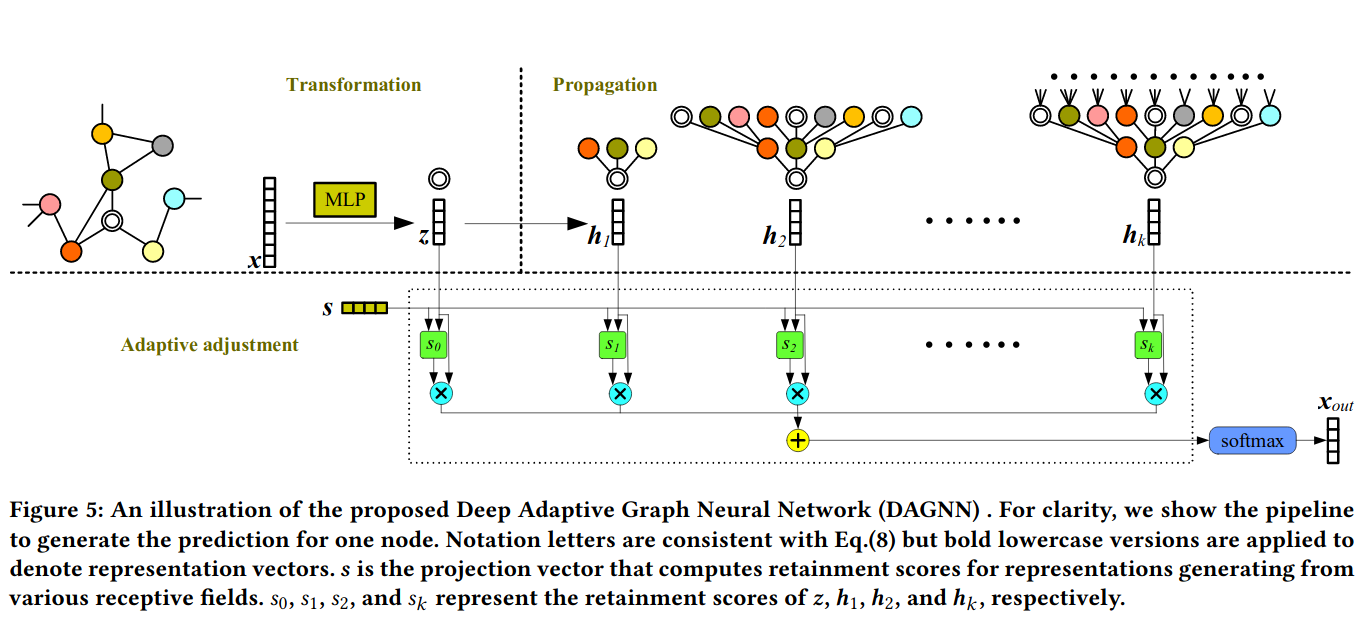
\includegraphics[width=0.8\paperwidth]{dagnn-arch.png}
\end{figure}
\subsection{Smoothness Metrics}

使用欧式距离为相似度度量 
\begin{equation}
    D\left(\boldsymbol{x}_{i}, \boldsymbol{x}_{j}\right)=\frac{1}{2}\left\|\frac{\boldsymbol{x}_{i}}{\left\|\boldsymbol{x}_{i}\right\|}-\frac{\boldsymbol{x}_{j}}{\left\|\boldsymbol{x}_{j}\right\|}\right\|,
\end{equation}
点到图的平滑度
\begin{equation}
    S M V_{i}=\frac{1}{n-1} \sum_{j \in V, j \neq i} D\left(x_{i}, x_{j}\right)
\end{equation}
图的总平滑度度量
\begin{equation}
    S M V_{G}=\frac{1}{n} \sum_{i \in V} S M V_{i}
\end{equation}

GCN随着层数增加,特征的平滑度缓慢下降, 但准确度迅速下降(数层). 这可能是由于propag. 和特征变换的耦合导致的. 解耦了的SGC则在75-100层以后准确度/平滑度迅速下降(over-smoothing问题).


\subsection{Convergence of Propagation}
\begin{theorem}
    给定图G, $\widehat{A}_{\oplus}=\widetilde{D}^{-1} \widetilde{A} \text { and } \widehat{A}_{\odot}=\widetilde{D}^{-\frac{1}{2}} \widetilde{A} \widetilde{D}^{-\frac{1}{2}}
    $, $\Psi(x)=\frac{x}{sum(x)}, \Phi(x)=\frac{x}{||x||}$.
    $$
    \lim _{k \rightarrow \infty} \widehat{A}_{\oplus}^{k}=\Pi_{\oplus}
    $$,
    其中$\Pi_{\oplus}$每行都是$$
    \pi_{\oplus}=\Psi(e \bar{D})
    $$
\end{theorem}

\begin{theorem}
    给定图G, $$
    \lim _{k \rightarrow \infty} \widehat{A}_{\odot}^{k}=\Pi_{\odot}
    $$, 其中$$
    \Pi_{\odot}=\Phi\left(\tilde{D}^{\frac{1}{2}} e^{T}\right)\left(\Phi\left(\tilde{D}^{\frac{1}{2}} e^{T}\right)\right)^{T}
    $$
\end{theorem}

这两个定理说明了,如果使用无限层的propagation, 会导致传递矩阵的收敛和退化, 进而导致不可分的feat. repr./ over-smoothing. 这不可避免的是一个问题, 所以我们应该更加关心收敛速度.

\subsection{DAGNN: Deep Adaptive GNN}

DAGNN的结构如下
\begin{equation}
    \begin{array}{ll}
    Z=\operatorname{MLP}(X) & \in \mathbb{R}^{n \times c} \\
    H_{\ell}=\widehat{A}^{\ell} Z, \ell=1,2, \cdots, k & \in \R^{n \times c}\\
    H=\operatorname{stack}\left(Z, H_{1}, \cdots, H_{k}\right) & \in \mathbb{R}^{n \times c} \\
    S=\sigma(H s)& \in \R^{n \times (k+1) \times 1} \\
    \tilde{S}=\text { reshape }(S) & \in \R^{n \times 1 \times  (k+1)} \\
    X_{\text {out}}=\operatorname{softmax}(\text { squeeze }(\tilde{S} H)) & \in \mathbb{R}^{n \times(k+1) \times c} \\
    \end{array}
\end{equation}
这里使用对称正规化的传播矩阵(GCN-like), $s\in \R^{c\times 1}$是(小型嵌入式MLP中的)的可训练的投影向量(计算出的$\tilde S$为赋予不同大小receptive fields的特征向量权重). DAGNN没有FC层! 输出就直接为类别预测分数.

\section{t-SNE(t-Distributed Stochastic Neighbor Embedding)}

\subsection{SNE}

\bt{Target} $f:X\to Y\in R^{3 or 2}$, 一个降维映射

将欧式距离变为条件概率$p_{j|i}$, 常用的概率如归一化的Gaussian
\begin{equation}
    p_{j \mid i}=\frac{\exp \left(-\left\|x_{i}-x_{j}\right\|^{2} / 2 \sigma_{i}^{2}\right)}{\sum_{k \neq i} \exp \left(-\left\|x_{i}-x_{k}\right\|^{2} / 2 \sigma_{i}^{2}\right)}
\end{equation}
并且设置为自身相似度为0:$p_{i|i}=0$

在低维度下的相似度也类似定义,并固定方差为$1/\sqrt{2}$
\begin{equation}
    q_{j \mid i}=\frac{\exp \left(-\left\|y_{i}-y_{j}\right\|^{2} \right)}{\sum_{k \neq i} \exp \left(-\left\|y_{i}-y_{k}\right\|^{2}\right)}
\end{equation}

则优化变化前后的两个分布的KL散度
\begin{equation}
    C=\sum_{i} K L\left(P_{i} \mid Q_{i}\right)=\sum_{i,j} p_{j \mid i} \log \left\{\frac{p_{j \mid i}}{q_{j \mid i}}\right\}
\end{equation}

困惑度(perpleixity)
\begin{equation}
    \operatorname{Perp}\left(P_{i}\right)=2^{H\left(P_{i}\right)}\\
    H\left(P_{i}\right)=-\sum_{j} p_{j \mid i} \log _{2} p_{j \mid i}
\end{equation}
用于选择方差. 使用二分搜索困惑度指标找到最优方差.

在优化开始阶段可以加入一些Gaussian noise, 之后如同退火逐渐减少噪声幅度, 可以避免局部最优解. 无法避免crowding问题.

\subsection{UNI-SNE}

给低维空间一个均匀分布基准. 可通过退火逐渐减小这个基准

\subsection{t-SNE}

使用对称的联合pdf$p_{ij}=\frac{1}{2}(p_{i|j}+p_{j|i})$来解决不对称性. 同时低维分布改为t-分布
\begin{equation}
    f(t)=\frac{\Gamma\left(\frac{v+1}{2}\right)}{\sqrt{v \pi} \Gamma\left(\frac{v}{2}\right)}\left(1+\frac{t^{2}}{v}\right)^{-\frac{v+1}{2}}
\end{equation}
$v=1$时为Cauchy分布$$f(t)=\frac{1}{\pi (1+t^2)}$$.

\bt{Tricks} \begin{itemize}
    \item 提前压缩: 开始初始化时点离得近些, 方便聚类中心移动. 可通过L2正则项的引入实现?
    \item 提前夸大: 开始优化阶段$p_{ij}$进行扩大, 避免太小导致优化太慢 
\end{itemize}

\bt{Cons} \begin{itemize}
    \item 主要用于可视化, 难以用于特征提取.
    \item 倾向于保存局部特征. 对于内蕴维度(intrinstic dim.)较高的数据集不可能完整映射.
    \item 没有唯一解. 没有预估. 训练太慢($O(n^2)$), 后续有基于树的改进.
\end{itemize}

\subsection{Barnes-Hut-SNE}

\subsubsection{Approximating Input Simularities by Vantage-point Tree}

使用一定数量的最近邻而非全部点, 来估计相似度.
\begin{equation}
    \begin{array}{c}
    p_{j \mid i}=\left\{\begin{array}{cc}
    \frac{\exp \left(-d\left(\mathbf{x}_{i}, \mathbf{x}_{j}\right)^{2} / 2 \sigma_{i}^{2}\right)}{\sum_{k \in \mathcal{N}_{i}} \exp \left(-d\left(\mathbf{x}_{i}, \mathbf{x}_{k}\right)^{2} / 2 \sigma_{i}^{2}\right)}, & \text { if } j \in \mathcal{N}_{i} \\
    0, & \text { otherwise }
    \end{array}\right. \\
    p_{i j}=\frac{p_{j \mid i}+p_{i \mid j}}{2 N}
    \end{array}
\end{equation}

最近邻集合的选取可以通过VPT来找到,时间代价为$O(u N\log N)$, $u$为perplexity.

一个VPT中,每个节点保存了一个数据对象和一个以其为中心的球. 所有非叶节点都有两个孩子, 左儿子保存了所有在球内部的数据对象, 右儿子则保存了所有在外的数据对象. VPT通过一个一个遍历数据对象构建, 每次根据在外/内便利节点, 并且创建新节点, 其半径为父节点所有对象到他的距离中位数.

一次最近邻搜索可以用VPT上的DFS来实现, 计算所有节点到目标节点的距离, 维护已经找到的最近邻和到最远近邻的距离$\tau$. $\tau$决定了是否要继续探索: 若左节点里可能有比它更近的节点, 搜索左节点, 右边节点同理. 若目标节点在左节点的球中, 先搜索左节点, 右边同理.

\subsubsection{Approximating t-SNE Gradients}

有
\begin{equation}
    \frac{\partial C}{\partial \mathbf{y}_{i}}=4\left(F_{\text {attr}}-F_{\text {rep}}\right)=4\left(\sum_{j \neq i} p_{i j} q_{i j} Z\left(\mathbf{y}_{i}-\mathbf{y}_{j}\right)-\sum_{j \neq i} q_{i j}^{2} Z\left(\mathbf{y}_{i}-\mathbf{y}_{j}\right)\right)
\end{equation}
前半部分可以方便的算出, 后半部分可利用Barnes-Hut算法快速近似, $O(N \log N)$.

考虑两个点$y_j,y_k$很接近, 那么他们在$y_i$梯度中的贡献就很相近. BH算法利用这一点, 在embed. dist. 上建立一个quad-tree来估计总梯度. 

Quad-Tree是一个树, 每个节点代表了一个矩形, 非叶节点有四个子节点, 代表了划分为个象限的四个矩形. 叶节点包含最多一个embedding点. 在每个节点, 保存矩形的质心$y_{cell}$,和总包含点数. 一个N个点的quad-tree可以在$O(N)$时间构建. 每个cell中对总梯度的贡献相似, 所以
\begin{equation}
    \sum_{j\in cell}q_{i j}^{2} Z\left(\mathbf{y}_{i}-\mathbf{y}_{j}\right)\approx N_{\text {cell}} q_{i, \text {cell}}^{2} Z\left(\mathbf{y}_{i}-\mathbf{y}_{\text {cell}}\right)
\end{equation}
并且定义单元配分函数
\begin{equation}
    q_{i, c e l l} Z=\left(1+\left\|\mathbf{y}_{i}-\mathbf{y}_{\text {cell}}\right\|^{2}\right)^{-1}
\end{equation}
定义trade-off factor, 衡量一个单元是否可以作为整体参与计算
\begin{equation}
    \left\|\mathbf{y}_{i}-\mathbf{y}_{\text {cell}}\right\|^{2} / r_{\text {cell}}<\theta
\end{equation}\footnote{
    In other words, more easy to comprehend:
    $$
    r_{cell}> ||y_i-y_{cell}||^2/\theta
    $$
    则不行
}

Dual-Tree Algorithms: 使用cell-cell距离来进一步减少计算.

\section{Autoregressive Flows}

Planar Flow
\begin{equation}
    f(\mathbf{z})=\mathbf{z}+\mathbf{u} h\left(\mathbf{w}^{T} \mathbf{z}+b\right)
\end{equation}
行列式为
\begin{equation}
    \left|\operatorname{det} \frac{\partial f}{\partial \mathbf{z}}\right|=\left|1+\mathbf{u}^{T} h'(\bs w^T \bs z+b)\bs w\right|
\end{equation}
可以看做空间中的超平面, 收缩或者扩张其附近的空间.

Radial Flow
\begin{equation}
    f(\mathbf{z})=\mathbf{z}+\beta h(\alpha, r)\left(\mathbf{z}-\mathbf{z}_{0}\right)
\end{equation}
其中$r=||\bs z-\bs z_0||_2, h(\alpha, r) = \frac{1}{\alpha+r}$
类似的, 可以看作超空间的一个球, 收缩或者扩张其中的空间.

由于这些都是比较sparse的变换,只影响空间的一小部分,需要很多层才能对高维空间有效.

\subsection{Autoregressive Transformation}

使用per-dim的AF
\begin{equation}
    \begin{array}{c}
    y_{1}=\mu_{1}+\sigma_{1} z_{1} \\
    y_{i}=\mu\left(\mathbf{y}_{1: i-1}\right)+\sigma\left(\mathbf{y}_{1: i-1}\right) z_{i}
    \end{array}
    \label{MAF}
\end{equation}
Jacobian是下三角矩阵, 行列式容易计算
\begin{equation}
    |det J| = \left|\prod_i \sigma(\bs y_{1:i-1})\right|
\end{equation}
逆变换为
\begin{equation}
    z_{i}=\frac{y_{i}-\mu\left(\mathbf{y}_{1: i-1}\right)}{\sigma\left(\mathbf{y}_{1: i-1}\right)}
    \label{IAF}
\end{equation}
由于无法并行计算所有维度, 必须顺序计算, 计算代价很高.

\subsection{MAF: Masked Autoregressive Flow}

MAF用上文中的公式\eqref{MAF}进行变换, 这导致了他采样时极为缓慢. 在图像生成中尤为如此, 不过作为VAE的先验倒是可以接受(如1000维).

\subsection{IAF: Inverse Autoregressive Flow}

IAF使用\eqref{IAF}来进行重参数化pdf. 使用之前的逆变换作为变换
\begin{equation}
    y_{i}=z_{i} \sigma\left(\mathbf{z}_{1: i-1}\right)+\mu\left(\mathbf{z}_{1: i-1}\right)
\end{equation}
此时所有的$\sigma,\mu$可以并行获得! i.e.
\begin{equation}
    \mathbf{y}=\mathbf{z} \circ \sigma(\mathbf{z})+\mu(\mathbf{z})
\end{equation}
假设$\bs z_{k}=\bs z, \bs z_{k+1} = \bs y$,则有
\begin{equation}
    \frac{\partial \mathbf{z}_{k}}{\partial \mathbf{z}_{k-1}}=\underbrace{\frac{\partial \mu_{k}}{\partial \mathbf{z}_{k-1}}+\frac{\partial \sigma_{k}}{\partial \mathbf{z}_{k-1}} \operatorname{diag}\left(\mathbf{z}_{k-1}\right)}_{\text {lower triangular with zeros on the diagonal }}+\operatorname{diag}\left(\sigma_{k}\right) \underbrace{\frac{\partial \mathbf{z}_{k-1}}{\partial \mathbf{z}_{k-1}}}_{=\mathbf{I}}
\end{equation}
以及行列式
\begin{equation}
    \operatorname{det}\left(\frac{\partial \mathbf{z}_{k}}{\partial \mathbf{z}_{k-1}}\right)=\prod_{i=1}^{d} \sigma_{k, i}
\end{equation}
最终log-pdf可以写作
\begin{equation}
    \log q_{K}\left(\mathbf{z}_{k}\right)=\log q(\mathbf{z})-\sum_{k=0}^{K} \sum_{i=1}^{d} \log \sigma_{k, i}
\end{equation}
由于他的逆是MAF, 所以从目标分布倒过来求density需要计算所有逆, 这就和MAF一样难于计算, 虽然仍是可能的.

\subsection{Sylvester NF(UAI 18')}

\subsubsection{Idea}
考虑单层MLP作为流
\begin{equation}
    \mathbf{z}^{\prime}=\mathbf{z}+\mathbf{A} h(\mathbf{B} \mathbf{z}+\mathbf{b})
\end{equation}
Jacobian可以从Sylvester行列式恒等式推出. Sylvester恒等式指出, 对于矩阵$\mathbf{A} \in \mathbb{R}^{D \times M}, \mathbf{B} \in \mathbb{R}^{M \times D}$,有
\begin{equation}
    \operatorname{det}\left(\mathbf{I}_{D}+\mathbf{A} \mathbf{B}\right)=\operatorname{det}\left(\mathbf{I}_{M}+\mathbf{B A}\right)
\end{equation}
据此,上述MLP的Jacobian行列式为
\begin{equation}
    \operatorname{det}\left(\frac{\partial \mathbf{z}^{\prime}}{\partial \mathbf{z}}\right)=\operatorname{det}\left(\mathbf{I}_{M}+\operatorname{diag}\left(h^{\prime}(\mathbf{B} \mathbf{z}+\mathbf{b})\right) \mathbf{B} \mathbf{A}\right)
\end{equation}

\subsubsection{Parametrization of A \& B}
一般来说,MLP作为流不是可逆的, 提出以下特例
\begin{equation}
    \mathbf{z}^{\prime}=\mathbf{z}+\mathbf{Q} \mathbf{R} h\left(\tilde{\mathbf{R}} \mathbf{Q}^{T} \mathbf{z}+\mathbf{b}\right)=\phi(\mathbf{z})
\end{equation},
其中$\bs R, \tilde{\bs R}$是上三角矩阵, $\bs Q=(\bs q_1...\bs q_M)$是一个正交基构成的矩阵/正交矩阵. 则Jacobian行列式变为
\begin{equation}
    \begin{aligned}
    \operatorname{det} \mathbf{J} &=\operatorname{det}\left(\mathbf{I}_{M}+\operatorname{diag}\left(h^{\prime}\left(\tilde{\mathbf{R}} \mathbf{Q}^{T} \mathbf{z}+\mathbf{b}\right)\right) \tilde{\mathbf{R}} \mathbf{Q}^{T} \mathbf{Q} \mathbf{R}\right) \\
    &=\operatorname{det}\left(\mathbf{I}_{M}+\operatorname{diag}\left(h^{\prime}\left(\tilde{\mathbf{R}} \mathbf{Q}^{T} \mathbf{z}+\mathbf{b}\right)\right) \tilde{\mathbf{R}} \mathbf{R}\right)
    \end{aligned}
\end{equation}
可以在O(M)时间内计算.

给出以上流的可逆性条件
\begin{theorem}
    以上流是可逆的, 若满足
    $$
    r_{ii}\tilde r_{ii} > -\frac{1}{||h'||_\infty}
    $$
\end{theorem}

\subsubsection{Preserving Orthogonality of Q}

生成一个正交矩阵不总是可行的! 下面介绍两个显式可微地构建正交矩阵的方法, 和一个使用permut-mat. 的方法.

\bt{Orthogonal Sylvester Flows/O-SNF} 使用如下可微变换
\begin{equation}
    \mathbf{Q}^{(k+1)}=\mathbf{Q}^{(k)}\left(\mathbf{I}+\frac{1}{2}\left(\mathbf{I}-\mathbf{Q}^{(k) \top} \mathbf{Q}^{(k)}\right)\right)
\end{equation}
一个充分收敛性条件
\begin{equation}
    \left\|\mathbf{Q}^{(0) \top} \mathbf{Q}^{(0)}-\mathbf{I}\right\|_{2}<1
\end{equation}
在本文实验中, 进行迭代直到
\begin{equation}
    \left\|\mathbf{Q}^{(k) \top} \mathbf{Q}^{(k)}-\mathbf{I}\right\|_{F} \leq \epsilon
\end{equation}
实验中大概会进行30次左右, 为了提高性能, 对所有流并行地计算这个正交化过程.

\bt{Householder Sylvester Flows/H-SNF}

Householder reflection, with respect to $\bs v\in \R^D$
\begin{equation}
    H(\mathbf{z})=\mathbf{z}-2 \frac{\mathbf{v} \mathbf{v}^{T}}{\|\mathbf{v}\|^{2}} \mathbf{z}
\end{equation}\footnote{
    In matrix sense, \begin{equation}
        H_{\bs z}=\bs I-\frac{2\bs v \bs v^T}{||\bs v||^2}
    \end{equation}
}
具体使用的Householder reflection数量是一个超参数, 而且要求$M=D$, 因为它使用的是方阵.

\bt{Traingular Sylvester Flows/T-SNF}

考虑为一个三角阵, 其中每个正交阵都在恒等矩阵和逆转$z$顺序的permut-mat. 之间转换(??),这等同于在每个流之间交换$\bs R, \tilde{\bs R}$的上下三角性.

\section{Contrastive Multi-view Representation Learning/MVRLG(ICML 20')}
\begin{figure}[htbp]
    \centering
    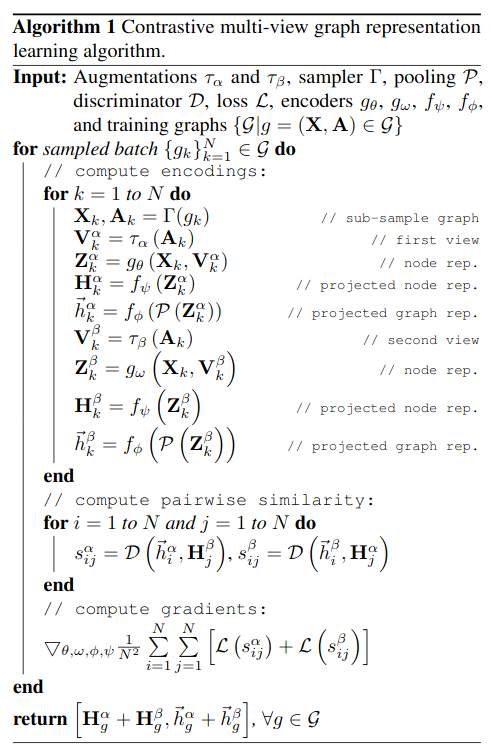
\includegraphics[width=0.6\paperwidth]{contrast-graph-alg.png}
\end{figure}
\bt{Idea} 使用图上的扩散来生成增强图. 通过网络两个view得到不同的repr., 让他们contrast/作为正负样本. 来源于CV的对比学习(使用congrent/incongruent views).

可以考虑两种图增强: 初始feature上的增强(如masking/加入Gaussian noise), 和图结构上的增强(增减连接性, 降采样, 从最短距离或扩散矩阵生成全局view). 前者往往会降低性能 \tRarr 使用全局图+降采样.

\subsection{Augmentations}
\begin{flushleft}
Diffusion:
\begin{equation}
    \mathbf{S}=\sum_{k=0}^{\infty} \Theta_{k} \mathbf{T}^{k} \in \mathbb{R}^{n \times n}
\end{equation},
假设$\sum_k \theta_k =1$, 其中$\bs T$是广义转移矩阵.
在PRR(Personal Page Rank)和heat kernel算法中, 
\begin{align}
    &\bs T = \bs A \bs D^{-1}, \\
    &\theta_k=\alpha(1-\alpha)^k\text{(Geometric!)}, or \theta_k = e^{-t}t^k/k!\text{(Poisson!)}
\end{align}
其中$\alpha$可以看传送概率, $t$可以看做扩散时间. 可以得到闭形式的解:
\begin{equation}
    \begin{array}{c}
    \mathbf{S}^{\text {heat }}=\exp \left(t \mathbf{A} \mathbf{D}^{-1}-t\right) \\
    \mathbf{S}^{\text {PPR }}=\alpha\left(\mathbf{I}_{n}-(1-\alpha) \mathbf{D}^{-1 / 2} \mathbf{A} \mathbf{D}^{-1 / 2}\right)^{-1}
    \end{array}
\end{equation}

关于降采样, 从一个view中采样, 并从另一个view中取相同的node和edges.
\end{flushleft}

\subsection{Encoders}
\begin{flushleft}
使用GCN作为基准encoder, 对于两个view使用分别的编码器$g_\theta, g_\omega$, 使用邻接/扩散矩阵作为两个全等的结构视图. 其中邻接矩阵上的GCN使用对称正则化($\tilde{\mathbf{A}}=\hat{\mathbf{D}}^{-1 / 2} \hat{\mathbf{A}} \hat{\mathbf{D}}^{-1 / 2},\hat{\mathbf{A}}=\mathbf{A}+\mathbf{I}_{\mathrm{N}}$), 并且使用PReLU函数作为非线性. GCN之后接着两层MLP得到图(节点)表示.

使用图池化提取全局特征(readout): 通过(JK-Net like)concat所有GCN层的点特征的和, 并送到单层MLP中
\begin{equation}
    \vec{h}_{g}=\sigma\left(\Vert_{l=1}^{L}\left[\sum_{i=1}^{n} \vec{h}_{i}^{(l)}\right] \mathbf{W}\right) \in \mathbb{R}^{h_{d}}
\end{equation}
本实验中比更复杂的readout好(如DiffPool)效果并不比这个好. 再送到共享的proj. head, 一个双层MLP中.

\end{flushleft}

\subsection{Training}
\begin{flushleft}
使用Deep InfoMax, 并且最大化两个视图的MI
\begin{equation}
    \max _{\theta, \omega, \phi, \psi} \frac{1}{|\mathcal{G}|} \sum_{g \in \mathcal{G}}\left[\frac{1}{|g|} \sum_{i=1}^{|g|}\left[\operatorname{MI}\left(\vec{h}_{i}^{\alpha}, \vec{h}_{g}^{\beta}\right)+\operatorname{MI}\left(\vec{h}_{i}^{\beta}, \vec{h}_{g}^{\alpha}\right)\right]\right]
\end{equation}
MI使用一个判别器来建模
$$
\mathcal{D}(., .): \mathbb{R}^{d_{h}} \times \mathbb{R}^{d_{h}} \longmapsto \mathbb{R}
$$
最简单的,可以使用内积作为相似度度量.

使用联合分布来做为正样本分布, 边缘分布的乘积作为负样本(即取不同图的视图作为负contrast)

\end{flushleft}

\section{GCC: Graph Contrastive Coding for GNN Pre-Training(KDD 20')}

\bt{Note} 本工作使用的是结构特征, 没有用节点特征. 用于更好的预测未见过的图: 完全的transfer across domains.

\subsection{GCC Pre-Training}
\begin{figure}[htbp]
    \centering
    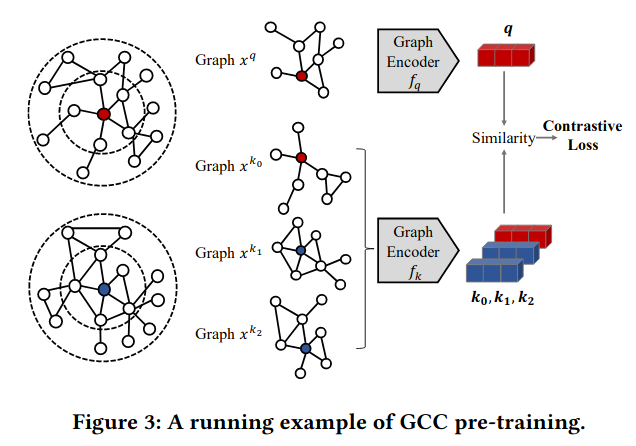
\includegraphics[width=0.6\textwidth]{gcc-fig.png}
\end{figure}
\begin{flushleft}

\bt{Idea} 使用subgraph instance-discrimination + InfoNCE! 对于记录了一堆encoded keys的dict$\left\{k_{0}, \cdots, k_{K}\right\}$, 和新编码的query$\bs q$,contrast learning找到一个匹配的code$\bs k_+$,可以计算InfoNCE
\begin{equation}
    \mathcal{L}=-\log \frac{\exp \left(\boldsymbol{q}^{\top} \boldsymbol{k}_{+} / \tau\right)}{\sum_{i=0}^{K} \exp \left(\boldsymbol{q}^{\top} \boldsymbol{k}_{i} / \tau\right)}
\end{equation}

使用子图作为对比学习中的instance!
\begin{definition}
    r-ego network $G_v$是一个距离节点$v$最短距离$\le r$的节点的诱导子图. (difference with r-hop?)
\end{definition}
GCC把不同r-ego net.作为不相似实例.

在CV中,两个经过不同aug.的图片作为了相似inst. pair, GCC中,同样考虑同个r-ego net. 的不同数据增强作为相似实例对, 并且使用图采样作为数据增强. 具体上讲, GCC使用三步: 带重启的随机游走, 子图诱导, 匿名化. 前两步的结果即ISRW(Induced Subgraph Random Walk Sampling). 最后一步匿名化把节点重新标号. 最后,两个经过如此图采样的方法被认为是相似实例对.

GCC理论上使用任何GNN都可以(作为encoder), 本文使用GIN(Graph Isomophism Net.), 当前的SOTA GNN. 由于大多数GNN使用节点feature作为输入, 使用generalized positional embedding(*GPE abbr.)

\begin{definition}
    GPE. 对于每个子图, 其GPE为正则化Laplacian的主要eig-vecs. 即, 在正则化Laplacian上进行EVD:
    \begin{equation}
        I-D^{-1 / 2} A D^{-1 / 2}=U \Lambda U^{\top}
    \end{equation}
    并取top eig-vecs作为GPE.
    (Question: EVD不唯一)
\end{definition}

GPE受到NLP的Transformer的启发. 此外还增加了one-hot编码的节点度, 以及binary的是否为中心节点的特征.

训练上, 由于维护一个字典代价很高, 所以使用一些别的方法来计算contrast, 如E2E(end-to-end)和MoCo(momentum constrast). \begin{itemize}
    \item E2E使用mini-batch,并把batch内的所有instance作为dictionary. Drawback: 词典大小受限与batch大小.
    \item MoCo使用基于momentum更新的$f_k$: 
    $$
    \theta_k = \rho \theta_k + (1-\rho)\theta_q
    $$
\end{itemize}

\end{flushleft}
\subsection{Finetuning GCC}
\begin{flushleft}
\begin{itemize}
    \item 对于graph-level下游任务, 使用图特征即可. 对于node-level下游任务, 使用r-ego net.的特征即可.
    \item 可以freeze/full fine-tune.
    \item GCC作为一个局部探索算法, 可以应用于大规模图和并行计算.
\end{itemize}
\end{flushleft}

\section{GIN: Graph Isomorphism Network(ICLR 19')}

\subsection{Weisfeiler-Lehman Test}
图同构还没有多项式时间算法. WL算法是一个高效的近似算法, 它在每个节点上聚合邻接节点的label, 然后hash为唯一的新label. 若在某个层面上label不同,则说明graph不同. WL子树kernel把每一次聚合的label作为某个子树(的数据).

\subsection{Math Intuitions}

\begin{lemma}
    若一个GNN把两个非同构图映射为不同表示, 则WL测试也把他们区分为非同构的.
\end{lemma}

这意味着所有给予聚合的GNN都最多和WL测试一样强(在区分非同构图上). 而且, 如果聚合操作和图readout函数都是单射,则和WL测试同样强.

\begin{theorem}
    Let $\mathcal{A}: \mathcal{G} \rightarrow \mathbb{R}^{d}$ be a GNN. With a sufficient number of GNN layers, $\mathcal{A}$ maps any graphs $G_{1}$ and $G_{2}$ that the Weisfeiler-Lehman test of isomorphism decides as non-isomorphic, to different embeddings if the following conditions hold:
    a) $\mathcal{A}$ aggregates and updates node features iteratively with
    $$
    h_{v}^{(k)}=\phi\left(h_{v}^{(k-1)}, f\left(\left\{h_{u}^{(k-1)}: u \in \mathcal{N}(v)\right\}\right)\right)
    $$
    where the functions $f$, which operates on multisets, and $\phi$ are injective.
    b) $\mathcal{A}$'s graph-level readout, which operates on the multiset of node features $\left\{h_{v}^{(k)}\right\},$ is injective.
\end{theorem}

\subsection{GIN}

下面的引理说明了sum-aggr是单射, 并且可以用于表示任意函数.
\begin{lemma}
    假设$\cal{X}$是可数的, 存在函数$f:\cal{X}\longmapsto \R^n$,使得$h(X)=\sum_{x\in X} f(x)$对于任何大小有界的multi-set唯一. 进一步, 任何multiset函数可以分解为$g(X)=\phi\left(\sum_{x \in X} f(x)\right)$.
\end{lemma}
然而, 常用的mean-aggr.不是单射.

\begin{corollary}
    假设$\cal{X}$是可数的, 存在函数$f:\cal{X}\longmapsto \R^n$,使得存在任意多$\epsilon$的选择(包括所有无理数), 使得$h(c, X)=(1+\epsilon)f(c)+\sum_{x\in X} f(x)$对于任何大小有界的multi-set对$(c, X)$唯一. 进一步, 任何bi-multiset函数可以分解为$g(c, X)=\varphi\left((1+\epsilon) \cdot f(c)+\sum_{x \in X} f(x)\right)$.
\end{corollary}

使用MLP近似函数$f,\varphi$, 而且直接表示他们的合成$f^{(k+1)} \circ \varphi^{(k)}$.
\begin{equation}
    h_{v}^{(k)}=\operatorname{MLP}^{(k)}\left(\left(1+\epsilon^{(k)}\right) \cdot h_{v}^{(k-1)}+\sum_{u \in \mathcal{N}(v)} h_{u}^{(k-1)}\right)
\end{equation}

\subsection{Graph Readout of GIN}

使用每一层级上的repr.(JK-Net like).
\begin{equation}
    h_{G}=\operatorname{CONCAT}\left(\operatorname{READOUT}\left(\left\{h_{v}^{(k)} \mid v \in G\right\}\right) \mid k=0,1, \ldots, K\right)
\end{equation}
根据已有定理, 如果READOUT函数是求和同一层中的feature, 则确实推广了WL.

\section{GraphLoG: Self-Supervised Represtation Learning with Local \& Global Structure}

\begin{figure}[htbp]
    \centering
    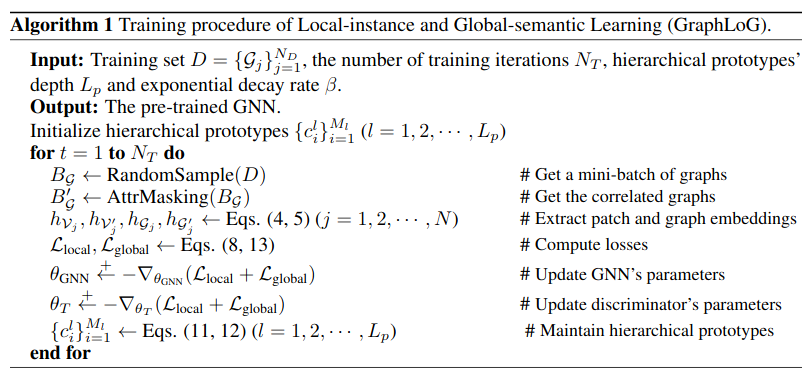
\includegraphics[width=0.75\textwidth]{graphlog-alg.png}
\end{figure}

\subsection{Preliminaries}

\bt{GNN and READOUT} GNN-layer
\begin{equation}
    h_{v}^{(l)}=\operatorname{COMBINE}^{(l)}\left(h_{v}^{(l-1)}, \text { AGGREGATE }^{(l)}\left(\left\{\left(h_{v}^{(l-1)}, h_{u}^{(l-1)}, X_{u v}\right): u \in \mathcal{N}(v)\right\}\right)\right)
\end{equation}
Graph Readout: 
\begin{equation}
    h_{\mathcal{G}}=\operatorname{READOUT}\left(\left\{h_{v} \mid v \in \mathcal{V}\right\}\right)
\end{equation}

\bt{Mutual Info. Est.} InfoNCE
\begin{equation}
    \mathcal{L}_{\mathrm{NCE}}\left(q, z_{+},\left\{z_{i}\right\}_{i=1}^{K}\right)=-\log \frac{\exp \left(T\left(q, z_{+}\right)\right)}{\exp \left(T\left(q, z_{+}\right)\right)+\sum_{i=1}^{K} \exp \left(T\left(q, z_{i}\right)\right)}
\end{equation}
其中T是某个参数化的判别函数.

\bt{RPCL: Rival Penalized Competitive Learning} 
RPCL在每个新样本上不仅推近winning cluster(最近聚类), 也推开rival cluster(次近聚类). 可以不预先指定聚类数地进行clustering.

\subsection{Local-Inst. Stru. Learning}

使用mask来获得相近(correlated)图. 对于每个mini-batch获得相近图(通过mask). 得到他们的node(patch)/graph repr.
\begin{equation}
    \begin{aligned}
    h_{\mathcal{V}_{j}}=\left\{h_{v} \mid v \in \mathcal{V}_{j}\right\} &=\operatorname{GNN}\left(X_{\mathcal{V}_{j}}, X_{\mathcal{E}_{j}}\right), \quad h_{\mathcal{V}_{j}^{\prime}}=\left\{h_{v} \mid v \in \mathcal{V}_{j}^{\prime}\right\}=\operatorname{GNN}\left(X_{\mathcal{V}_{j}^{\prime}}, X_{\mathcal{E}_{j}^{\prime}}\right) \\
    h_{\mathcal{G}_{j}} &=\operatorname{READOUT}\left(h_{\mathcal{V}_{j}}\right), \quad h_{\mathcal{G}_{j}^{\prime}}=\operatorname{READOUT}\left(h_{\mathcal{V}_{j}^{\prime}}\right)
    \end{aligned}
\end{equation}
最小化InfoNCE\footnote{如同其他contrast learning}
\begin{equation}
    \begin{array}{c}
    \mathcal{L}_{\text {patch }}=\frac{1}{\sum_{j=1}^{N}\left|\mathcal{V}_{j}^{\prime}\right|} \sum_{j=1}^{N} \sum_{v^{\prime} \in \mathcal{V}_{j}^{\prime}} \sum_{v \in \mathcal{V}_{j}} \mathbb{1}_{v \leftrightarrow v^{\prime}} \cdot \mathcal{L}_{\mathrm{NCE}}\left(h_{v^{\prime}}, h_{v},\left\{h_{\tilde{v}} \mid \tilde{v} \in \mathcal{V}_{j}, \tilde{v} \neq v\right\}\right) \\
    \mathcal{L}_{\text {graph }}=\frac{1}{N} \sum_{j=1}^{N} \mathcal{L}_{\mathrm{NCE}}\left(h_{\mathcal{G}_{j}^{\prime}}, h_{\mathcal{G}_{j}},\left\{h_{\mathcal{G}_{k}} \mid 1 \leqslant k \leqslant N, k \neq j\right\}\right) \\
    \mathcal{L}_{\text {local }}=\mathcal{L}_{\text {patch }}+\mathcal{L}_{\text {graph }}
    \end{array}
\end{equation}

\bt{Note} 同个batch中的其他图repr.作为negative instance. 同个图中其他node repr.作为negative instance.

\subsection{Global-Semantic Repr. Learning}

Graph(如分子图)常常有hierachical structure \trarr \textit{hierachical prototypes},建模图嵌入的分布. 他们是一些树的集合, 每个节点对应了一个prototype, 并且指向唯一的父节点(除非是根节点). 正式地, 这些节点是$\{c_i^l\}_{i=1}^{M_l},(l=1,2,...,L_p)$, 除了树叶节点, 每个节点都有一些子节点集合$\bm{C}(c_i^l)$.

\subsubsection{Init. of HP(Hirechichal Prototypes)}

先用$\cal{L}_{local}$预训练一个epoch, 利用这个GNN得到所有训练集中图的表示$\left\{h_{\mathcal{G}_{i}}\right\}_{i=1}^{N_{D}}$, 作为HP的叶子节点,并且使用RPCL得到底层的节点
\begin{equation}
    \left\{c_{i}^{L_{p}}\right\}_{i=1}^{M_{L_{p}}}=\operatorname{RPCL}\left(\left\{h_{\mathcal{G}_{i}}\right\}_{i=1}^{N_{D}}\right)
\end{equation}
之后RPCL被迭代的应用来得到整个HP树.

\subsubsection{Maintainance of HP}

训练过程中, 图嵌入在动态改变. 使用一下策略来更新HP:
\begin{enumerate}
    \item 每有一个batch训练完, 得到图embedding, 分成$M_{L_p}$个组(属于HP最底层聚类), 计算每一组的平均embedding. 并且更新节点上的embedding, 使用(momentum-like)指数移动平均更新模型
    \begin{equation}
        c_{i}^{L_{p}} \leftarrow \beta c_{i}^{L_{p}}+(1-\beta) \widehat{c}_{i}^{L_{p}}, \quad 1 \leqslant i \leqslant M_{L_{p}}
    \end{equation}
    此处$\beta$是衰减常数, 之后上层节点embedding更新为子节点的平均.
    \item 
\end{enumerate}

为了捕捉global-semantic structure, 让相关图属于同一聚类! 具体上讲, 对于每一个图$\cal{G}_j$, 使用cosine sim., 在每一层上寻找最接近的embedding
$$
s\left(\mathcal{G}_{j}\right)=\left\{s_{1}\left(\mathcal{G}_{j}\right), s_{2}\left(\mathcal{G}_{j}\right), \cdots, s_{L_{p}}\left(\mathcal{G}_{j}\right)\right\}
$$
这里要让相关图的embedding和这些repr.相近, 使用InfoNCE
\begin{equation}
    \mathcal{L}_{\text {global }}=\frac{1}{N \cdot L_{p}} \sum_{j=1}^{N} \sum_{l=1}^{L_{p}} \mathcal{L}_{\mathrm{NCE}}\left(h_{\mathcal{G}_{j}^{\prime}}, s_{l}\left(\mathcal{G}_{j}\right),\left\{c_{i}^{l} \mid 1 \leqslant i \leqslant M_{l}, c_{i}^{l} \neq s_{l}\left(\mathcal{G}_{j}\right)\right\}\right)
\end{equation}
即, 对于每一层, 正样本是那个(原图)最相近的embedding, 负样本是(原图)其他样本repr.

模型在每一个iteration上最小化全loss
\begin{equation}
    \min _{\operatorname{GNN}, T} \mathcal{L}_{\text {local }}+\mathcal{L}_{\text {global }}
\end{equation}

\subsection{Sup-GraphLoG: A Supervised Baseline}

使用label来简单监督学习, 作为baseline. 对于任何一个图, 找到在HP底层匹配的(随机的)一个匹配的prototype, 把搜索路径作为正样本, 再随机选择另一条不正确的路径作为负样本. 然后mini-batch上的全局loss为
\begin{equation}
    \mathcal{L}_{\mathrm{global}}^{\mathrm{sup}}=\frac{1}{N \cdot L_{p}} \sum_{j=1}^{N} \sum_{l=1}^{L_{p}} \mathcal{L}_{\mathrm{NCE}}\left(h_{\mathcal{G}_{j}}, s_{l}\left(\mathcal{G}_{j}\right), s_{l}^{n}\left(\mathcal{G}_{j}\right)\right)
\end{equation}


\section{Orthogonal Weights in DNNs}

\subsection{Formulation \& Good Properties}
\flushleft
优化参数, 使得权重是(伪)正交的
\begin{equation}
    \begin{aligned}
    \theta^{*}=& \arg \min _{\theta} \mathbb{E}_{(\mathbf{x}, \mathbf{y}) \in D}[\mathcal{L}(\mathbf{y}, f(\mathbf{x} ; \theta))] \\
    & \text { s.t. } \quad \mathbf{W}^{l} \in \mathcal{O}_{l}^{n_{l} \times d_{l}}, l=1,2, \ldots, L
    \end{aligned}
\end{equation}
此处伪正交矩阵在一个实Stiefel流形$\mathcal{O}_{l}^{n_{l} \times d_{l}}=\left\{\mathbf{W}^{l} \in \mathbb{R}^{n_{l} \times d_{l}}: \mathbf{W}^{l}\left(\mathbf{W}^{l}\right)^{T}=\mathbf{I}\right\}$上. \trarr OMDSM(Optim. on Multiple Depedent Stiefel Manifolds) Problem

好处
\begin{itemize}
    \item $\bs s = \bs W \bs x, \bs W\in \R^{n\times d}$, 若输入$\bs x$是白化了的, 则输出$\bs s$也是(0均值且分量不相关); 如果$n=d$,则$||\bs s|| = || \bs x ||$; 梯度相等$\left\|\frac{\partial \mathcal{L}}{\partial \mathbf{x}}\right\|=\left\|\frac{\partial \mathcal{L}}{\partial \mathbf{s}}\right\|$
    \item 自动地, 这正则化了权重. 减少了自由度(Stiefel Manifold的维度减少了): $\dim \mathcal{O}^{n\times d}=nd-n(n+1)/2$
\end{itemize}

\subsection{OWN: Orthogonal Weight Normalization}

\flushleft
使用Riemann(流形)优化算法(like in RNNs\footnote{
    What's that actually?
})导致了收敛的不稳定性/性能差. 显式地使用参数矩阵的重参数化
\begin{equation}
    \phi: \mathbb{R}^{n_{l} \times d_{l}} \rightarrow \mathbb{R}^{n_{l} \times d_{l}}
\end{equation}
并且$\phi(\bs V)=\bs W, s.t. \bs W\bs W^T=\bs I$.

使用一个线性变换来作为函数
\begin{align}
    \phi(\bs V)&=\bs P \bs V_C\\
    \bs V_C&= \bs V - \bs c \bs 1_d^T\\
    \bs c&= \frac{1}{d}\bs V\bs 1_d\\
    \text{which means} \bs V_C&=\bs V - \frac{1}{d} \bs V \bs E_d=\bs V(\bs I - \frac{1}{d}E_d)
\end{align}
使用以下变换来得到权重, 使得Jacobian的奇异值接近于1
\begin{equation}
    \begin{array}{c}
    \min _{\mathbf{P}} \operatorname{tr}\left(\left(\mathbf{W}-\mathbf{V}_{C}\right)\left(\mathbf{W}-\mathbf{V}_{C}\right)^{T}\right) \\
    \text { s.t. } \quad \mathbf{W}=\mathbf{P} \mathbf{V}_{C} \text { and } \mathbf{W} \mathbf{W}^{T}=\mathbf{I}
    \end{array}
    \label{ortho:1}
\end{equation}  
进而, 这个优化问题有closed form sol. 
\begin{equation}
    \mathbf{P}^{*}=\mathbf{D} \bm \Lambda^{-1 / 2} \mathbf{D}^{T}
\end{equation}
其中$\bs V_C \bs V_C^T=\bm \Sigma=\bs D\bm \Lambda \bs D^T$是协方差矩阵的EVD(SVD). 
最后的形式为
\begin{equation}
    \mathbf{W}=\phi(\mathbf{V})=\mathbf{D} \Lambda^{-1 / 2} \mathbf{D}^{T}\left(\mathbf{V}-\mathbf{c} \mathbf{1}_{d}^{T}\right)
\end{equation}
类似但没有最小化\eqref{ortho:1}的选择$\bs P_{var}=\bm \Lambda^{-1/2}\bs D^T$

\subsubsection{Backpropagation}

计算Jacobian
\begin{equation}
    \begin{aligned}
    \frac{\partial \mathcal{L}}{\partial \Lambda} &=-\frac{1}{2} \mathbf{D}^{T} \frac{\partial \mathcal{L}}{\partial \mathbf{W}} \mathbf{W}^{T} \mathbf{D} \Lambda^{-1} \\
    \frac{\partial \mathcal{C}}{\partial \mathbf{D}} &=\mathbf{D} \Lambda^{\frac{1}{2}} \mathbf{D}^{T} \mathbf{W} \frac{\partial \mathcal{L}}{\partial \mathbf{W}} \mathbf{D} \Lambda^{-\frac{1}{2}}+\frac{\partial \mathcal{L}}{\partial \mathbf{W}} \mathbf{W}^{T} \mathbf{D} \\
    \frac{\partial \mathcal{C}}{\partial \mathbf{S}} &=\mathbf{D}\left(\left(\mathbf{K}^{T} \odot\left(\mathbf{D}^{T} \frac{\partial \mathcal{L}}{\partial \mathbf{D}}\right)\right)+\left(\frac{\partial \mathcal{L}}{\partial \Lambda}\right)_{\operatorname{diag}}\right) \mathbf{D}^{T} \\
    \frac{\partial \mathcal{L}}{\partial \mathbf{c}} &=-\mathbf{1}_{d}^{T} \frac{\partial \mathcal{L}}{\partial \mathbf{W}} \mathbf{D} \Lambda^{-\frac{1}{2}} \mathbf{D}^{T}-2 \cdot \mathbf{1}_{d}^{T}\left(\mathbf{V}-\mathbf{c} \mathbf{1}_{d}^{T}\right)^{T}\left(\frac{\partial \mathcal{L}}{\partial \Sigma}\right)_{s} \\
    \frac{\partial \mathcal{L}}{\partial \mathbf{V}} &=\mathbf{D} \Lambda^{-\frac{1}{2}} \mathbf{D}^{T} \frac{\partial \mathcal{L}}{\partial \mathbf{W}}+2\left(\frac{\partial \mathcal{L}}{\partial \Sigma}\right)_{s}\left(\mathbf{V}-\mathbf{c} \mathbf{1}_{d}^{T}\right)+\frac{1}{d} \frac{\partial \mathcal{L}^{T}}{\partial \mathbf{c}} \mathbf{1}_{d}^{T}
    \end{aligned}
\end{equation}
此处
\begin{equation}
    \mathbf{K}_{i j}=\frac{1}{\sigma_{i}-\sigma_{j}}[i \neq j]
\end{equation}是一个对角线为0的矩阵.

\subsubsection{As Convolution}

\flushleft
卷积层的参数$\bs W^C\in \R^{n\times d\times F_h\times F_w}$, 以及上一层的输入特征$\bs X\in \R^{d\times h\times w}$, 那么activation可以计算为
\begin{equation}
    s_{k, \delta}=\sum_{i=1}^{d} \sum_{\tau \in \Omega} w_{k, i, \tau} h_{i, \delta+\tau}=\langle\mathbf{w}_{k}, \mathbf{h}_{\delta}\rangle
\end{equation}
此处使用$\bs W\in \R^{n\times p},p=d F_h F_w$作为总的filters.

\subsubsection{Group Based Orthogonalization: Divided Filters}

\flushleft
权重按行分为多组, 每组大小一致(为一个小数$N_G<d$,如64/128), 使得EVD的计算代价很小. 大大降低计算难度.

\section{OrthDNNs: Orthogonal DNNs(TPAMI 19')}

在数据分布$\cal Z=\cal X\times \cal Y$上, ML的目标是最优化期望风险
\begin{equation}
    R(f)=\mathbb{E}_{z \sim P}[\mathcal{L}(f(\boldsymbol{x}), y)]
\end{equation}
然而真实分布未知,所以用样本期望(训练集$S_m$)代替
\begin{equation}
    R_{m}(f)=\frac{1}{m} \sum_{i=1}^{m} \mathcal{L}\left(f\left(\boldsymbol{x}_{i}\right), y_{i}\right)
\end{equation}
统计学习的一大目标是计算泛化误差/gen. gap
\begin{equation}
    \mathrm{GE}\left(f_{S_{m}}\right)=\left|R\left(f_{S_{m}}\right)-R_{m}\left(f_{S_{m}}\right)\right|
\end{equation}
这里考虑由DNN建模的分类-表示模型(Class. Repr. Learning)
\begin{equation}
    \begin{aligned}
    R(f, T) &=\mathbb{E}_{z \sim P}[\mathcal{L}(f(T \boldsymbol{x}), y)] \\
    R_{m}(f, T) &=\frac{1}{m} \sum_{i=1}^{m} \mathcal{L}\left(f\left(T \boldsymbol{x}_{i}\right), y_{i}\right)
    \end{aligned}
\end{equation}

\subsection{GE Analysis in a Robustness and Isomeric Mapping Perspecitve}

\begin{definition}
    ($K,\epsilon(\cdot)$-robustness)对于$K\in \mathbb{N},\epsilon: \cal{Z}^m\mapsto \R$一个算法是$K,\epsilon(\cdot)$-robust的,如果$\cal Z$可以分为K个分离的集合, 记为$\mathcal{C}=\left\{C_{k}\right\}_{k=1}^{K}$, 且
    \begin{equation}
        \begin{array}{r}
        \forall s_{i}=\left(\boldsymbol{x}_{i}, y_{i}\right) \in C_{k}, \forall z=(\boldsymbol{x}, y) \in C_{k} \\
        \Longrightarrow\left|\mathcal{L}\left(f\left(\boldsymbol{x}_{i}\right), y_{i}\right)-\mathcal{L}(f(\boldsymbol{x}), y)\right| \leq \epsilon\left(S_{m}\right)
        \end{array}
    \end{equation}
\end{definition}

对于任何健壮的算法, 有以下定理\footnote{Huan Xu and Shie Mannor.  Robustness and generalization.Ma-chine Learning, 86(3):391–423, 2012.1,2,4,6,8}
\begin{theorem}
如果一个算法是($K,\epsilon(\cdot)$-robust, 并且一个损失函数$\cal L$是有界的,则
\begin{equation}
    \operatorname{Pr}\left(G E\left(f_{S_{m}}\right) \leq \epsilon\left(S_{m}\right)+M \sqrt{\frac{2 K \log (2)+2 \log (1 / \nu)}{m}}\right)\ge 1-\nu
\end{equation}.
\end{theorem}

\begin{definition}
    (Covering Number)给出一个度量空间$(\cal M, d)$, 集合$\hat S$是另一个集合$S$的$\gamma$-cover, 若$\forall s\in S, \exists \hat s\in \hat S, s.t. d(\hat s, s)\le \gamma$. 集合S的$\gamma$-covering number是
    \begin{equation}
        \mathcal{N}_{\gamma}(\mathcal{S}, \rho)=\min \{|\hat{\mathcal{S}}|: \hat{\mathcal{S}} \text { is a } \gamma \text { -covering of } \mathcal{S}\}
    \end{equation}
\end{definition}

\begin{definition}
    ($\delta$-isometry) 映射$T:\cal P\mapsto \cal Q$(其中$\cal P, \cal Q$度量空间)是$\delta$-保距的, 若
    \begin{equation}
        \forall \boldsymbol{x}, \boldsymbol{x}^{\prime} \in \mathcal{P},\left|\rho_{Q}\left(T \boldsymbol{x}, T \boldsymbol{x}^{\prime}\right)-\rho_{P}\left(\boldsymbol{x}, \boldsymbol{x}^{\prime}\right)\right| \leq \delta
    \end{equation}
\end{definition}

\begin{theorem}
    对与任何CRL问题的算法, 若$\cal L\circ f$(关于$\bs T \bs x$)的Lipschitz Constant有上界A, 且T是$\delta$-保距的,且$\cal X$是紧的, 且有covering number$\mathcal{N}_{\gamma / 2}(\mathcal{X}, \rho)$, 则这个算法是$\left(|\mathcal{Y}| \mathcal{N}_{\gamma / 2}(\mathcal{X}, \rho), A(\gamma+\delta)\right)$-robust.
\end{theorem}

\subsection{GE Analysis of DNN}

\footnote{
    TO READ AND MAKE NOTES
    % TODO
}

\subsection{OrthDNN by SVB(Singular Value Bound)}

类似于之前的一篇, 为在Stiefel流形上的约束优化. 可以通过流形上的SGD(切空间投影法)或者Frank-Wolfe算法(流形投影法). 太慢! 使用SVB来进行优化.

\begin{itemize}
    \item 使用估计的带偏移的梯度投影方向. 每隔一定数量迭代拉回到流形上.
    \item 考虑到DNN的优化问题含有巨大数量的局部极小/临界点. 在目标流形附近探索可能会得到更好的解(避免local minima/critical points)
    \item BN会改变权重矩阵的谱, 使得严格正交化的努力白费.
\end{itemize}

Algorithm Sketch(SVB)
\begin{enumerate}
    \item 使用普通的SGD来更新参数.
    \item 每隔一些epochs, 对于每一层, 使用SVD来clamp奇异值到$((1+\epsilon)^{-1}, 1+\epsilon)$: 
    \begin{align}
        \bs W &= \bs U \bm \Sigma \bs V^T\\
        \bs W&\leftarrow \bs U \bm \Sigma_{\epsilon-clamped} \bs V^T
    \end{align}
    .
\end{enumerate} 

还可以使用罚函数法来作为无约束优化问题优化(SoftRegu)
\begin{equation}
    \min _{\Theta=\left\{\boldsymbol{W}_{l}, \boldsymbol{b}_{l}\right\}_{l=1}^{L}} \mathcal{L}\left(\left\{\boldsymbol{x}_{i}, y_{i}\right\}_{i=1}^{m} ; \Theta\right)+\lambda \sum_{l=1}^{L}\left\|\boldsymbol{W}_{l}^{\top} \boldsymbol{W}_{l}-\boldsymbol{I}\right\|_{F}^{2}
\end{equation}
需要假设$n_l \ge n_{l-1}$, 为了放松这一假设, 使用自然1-范数/谱范数(SRIP)而不是Frobenius范数
\begin{equation}
    \min _{\Theta=\left\{\boldsymbol{W}_{l, b}\right\}_{l-1}^{L}} \mathcal{L}\left(\left\{\boldsymbol{x}_{i}, y_{i}\right\}_{i=1}^{m} ; \Theta\right)+\kappa \sum_{i}^{L} \sigma_{\max }\left(\boldsymbol{W}_{l}^{\top} \boldsymbol{W}_{l}-\boldsymbol{I}\right)
\end{equation}

\subsubsection{BN Compatibility}

BN实际上干了
\begin{equation}
\mathrm{BN}(\boldsymbol{h})=\bm \Upsilon \bm \Phi(\boldsymbol{h}-\boldsymbol{\mu})+\boldsymbol{\beta}
\end{equation}
其中$\bm \mu \in \R^n$是这一层n个神经元的(batch的)均值, 对角阵$\bm \Phi=\operatorname{Diag}(1/\phi_i)$是神经元输出的标准差倒数矩阵(加上小值来增加数值稳定性).
并且$\bm \Upsilon, \bm \beta$是可训练的对角矩阵和bias. 最终的均值和标准差由running average给出训练样本的总体估计.

但是乘上一个对角矩阵会导致原先的权重矩阵sig-val不再相等! 所以让可训练的对角阵和偏差在每层都相等\trarr 对于精确形式的OrhDNN, 使用DBN(Degenerate Batch Norm), 其中$\bar \phi = \frac{1}{n}\sum_n \phi_i$

对于approx. OrthDNN, 使用BBN(Bounded BN), 控制(通过clamp)$\{v_i/\phi_i\}$在均值$\alpha=\frac{1}{n}\sum_i \frac{v_i}{\phi_i}, v_i/\phi_i\in [\alpha(1+\epsilon)^{-1}, \alpha(1+\epsilon)]$内.

\subsubsection{On CNN: OrthDNN as Convolution}

对于CNN的某一层, 要求的参数形状为$n_{l} \times n_{l-1} \times n_{h} \times n_{w}$, 本作使用生成$n_{l} \times n_{l-1}n_{h}n_{w}$形状的参数矩阵来得到这些filter.

\section{SimCLR: A Simple Framework for Contrastive Learning of Visual Representations}

\begin{figure}[htbp]
    \centering
    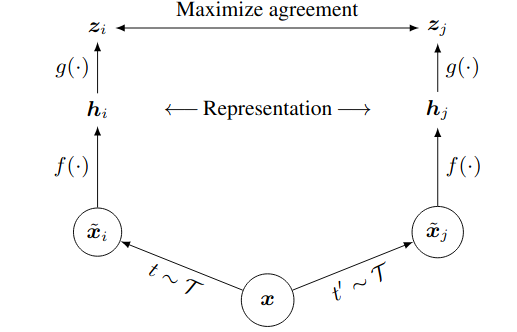
\includegraphics[width=0.75\textwidth]{simclr-alg.png}
\end{figure}

\subsection{Ideas \& Basics}

\begin{enumerate}
    \item 使用随机数据增强来得到两个相关视图:
    \begin{itemize}
        \item 随机剪裁/裁剪+缩放至原大小
        \item 随机色彩distortion
        \item 随机高斯模糊
        \item 没啥用的: cutoff, Sobel filters etc.
    \end{itemize}
    \item Encoder使用经典的ResNet结构.
    \item 一个小的MLP投影头(proj. head)用于投影到contrastive loss用于计算的空间.
    \item 在最后的特征空间上最小化InfoNCE(yet another \textit{contrastive loss}), 最大化相关图的MI
    \begin{equation}
        \ell_{i, j}=-\log \frac{\exp \left(\operatorname{sim}\left(z_{i}, z_{j}\right) / \tau\right)}{\sum_{k=1}^{2 N} \bm{1}_{[k \neq i]} \exp \left(\operatorname{sim}\left(\boldsymbol{z}_{i}, \boldsymbol{z}_{k}\right) / \tau\right)}
    \end{equation}
    其中相似度度量使用归一化点积(i.e. cosine similarity)$\operatorname{sim}(\boldsymbol{u}, \boldsymbol{v})=\boldsymbol{u}^{\top} \boldsymbol{v} /\|\boldsymbol{u}\|\|\boldsymbol{v}\|$
    其中负样本来自同一minibatch, $\tau$是温度系数.
\end{enumerate}

本方法没有利用类似MoCo的memory bank, 而是使用较大的batchsize(256-8192). SGD+Momemtum的优化器似乎和较大的batchsize上不稳定, 所以使用LARS优化器. 

使用Global BN: 在各个设备上本来BN的均值和方差是分别计算的, 这里在BN里使用聚合了所有设备的mean/variance. 其他方法包括在设备间shuffle samples, 或者使用layer norm\footnote{
    在MLP中, 归一化每一层的权重为期望0标准差1, 先计算均值和方差
    \begin{equation}
        \mu^{l}=\frac{1}{H} \sum_{i=1}^{H} w_{i}^{l} \quad \sigma^{l}=\sqrt{\frac{1}{H} \sum_{i=1}^{H}\left(w_{i}^{l}-\mu^{l}\right)^{2}}
    \end{equation}
    在计算FP前进行权重归一化
    \begin{equation}
        \hat{\mathbf{w}}^{l}=\frac{\mathbf{w}^{l}-\mu^{l}}{\sqrt{\left(\sigma^{l}\right)^{2}+\epsilon}}
    \end{equation}
    LN在权重够多的情况下和BN效果类似. 似乎在CNN上不能使用???
    \begin{remark}
        对于权重的更弱的限制(相比OrthDNN和OWN中近似正交化权重), 注意随机正交矩阵必然是归一化了的, 分量还是不相关的.
    \end{remark}
}而不是BN.

\section{BYOL: Build Your Own Latent}
\begin{figure}[htbp]
    \centering
    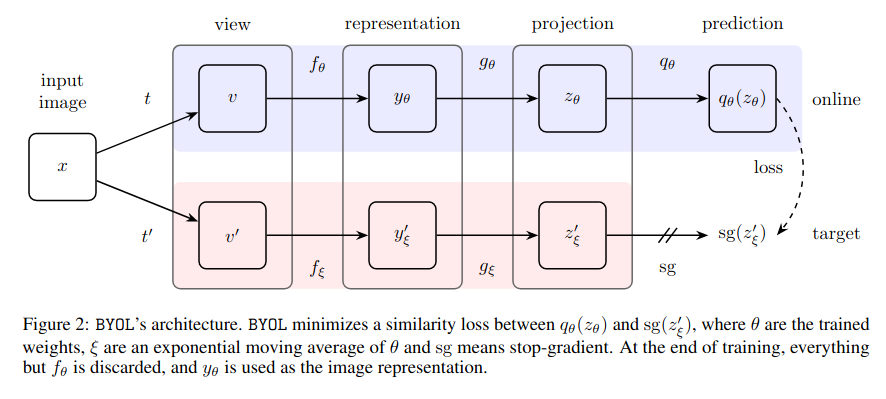
\includegraphics[width=\textwidth]{byol-fig.png}
\end{figure}
\subsection{Ideas \& Method}

使用两个网络来学习: online/target 网络, 每个网络都类似得由三个阶段组成:encoder $f_\theta$, proj. head $g_\theta$, predictor $q_\theta$(discriminator). online/target网络使用相同的结构,但是为不同的参数, 并且target网络的参数$\xi$是online参数$\theta$的moving average(under decay const. $\tau$)
\begin{equation}
    \xi \leftarrow \tau \xi+(1-\tau) \theta
\end{equation}

假设通过两个图像变换之后的view是$v,v'$, 然后我们使用要\underline{区分}两者的repr., 所以最小化负的cosine-simliarity\footnote{equivalent to MSE of normalized feature}
\begin{equation}
    \mathcal{L}_{\theta, \xi} \triangleq\left\|\overline{q_{\theta}}\left(z_{\theta}\right)-\bar{z}_{\xi}^{\prime}\right\|_{2}^{2}=2-2 \cdot \frac{\left\langle q_{\theta}\left(z_{\theta}\right), z_{\xi}^{\prime}\right\rangle}{\left\|q_{\theta}\left(z_{\theta}\right)\right\|_{2} \cdot\left\|z_{\xi}^{\prime}\right\|_{2}}
\end{equation}
同样的交换两个视图送到网络的顺序, 并且得到另一个loss, 加和来得到对称化loss
\begin{equation}
    \mathcal{L}_{\theta, \xi}^{\mathrm{BYDL}}=\mathcal{L}_{\theta, \xi}+\widetilde{\mathcal{L}}_{\theta, \xi}
\end{equation}
参数的更新
\begin{equation}
    \begin{array}{l}
    \theta \leftarrow \text { optimizer }\left(\theta, \nabla_{\theta} \mathcal{L}_{\theta, \xi}^{\mathrm{BYOL}}, \eta\right), \\
    \xi \leftarrow \tau \xi+(1-\tau) \theta
    \end{array}
\end{equation}

BYOL没有使用显式的方法防止mode collapse(negative samples etc.). 但是根据假设, 他们证明了, 至少在predictor是optimal的时候($q_\theta = q^\star$), 鞍点是不稳定的.

\section{MoCo: Momentum Contrast for Unsupervised Visual Representation Learning}
\begin{figure}[htbp]
    \centering
    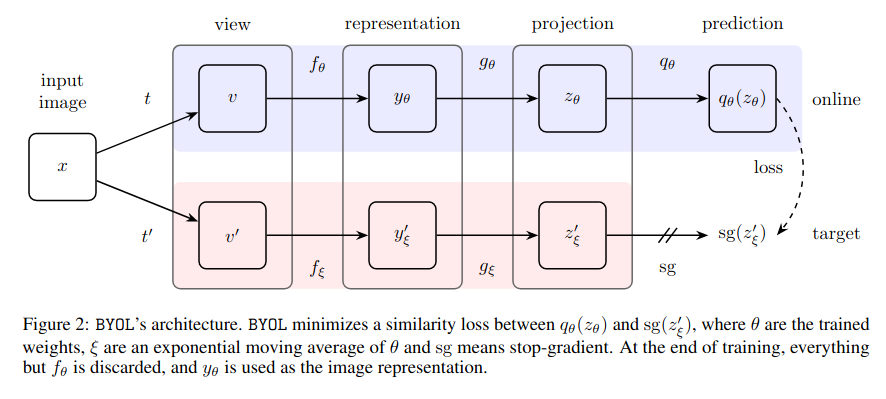
\includegraphics[width=\textwidth]{byol-fig.png}
\end{figure}
\subsection{Ideas \& Method}

InfoNCE on memory bank
\begin{equation}
    \mathcal{L}_{q}=-\log \frac{\exp (q \cdot k+/ \tau)}{\sum_{i=0}^{K} \exp \left(q \cdot k_{i} / \tau\right)}
\end{equation}

Momentum encoder: 按照moving average更新k-encoder
\begin{equation}
    \theta_{\mathrm{k}} \leftarrow m \theta_{\mathrm{k}}+(1-m) \theta_{\mathrm{q}}
\end{equation}

Tricks: Shuffling BNs

\section{SimSiam: Exploring Simple Siamese Representation Learning}
\begin{figure}[htbp]
    \centering
    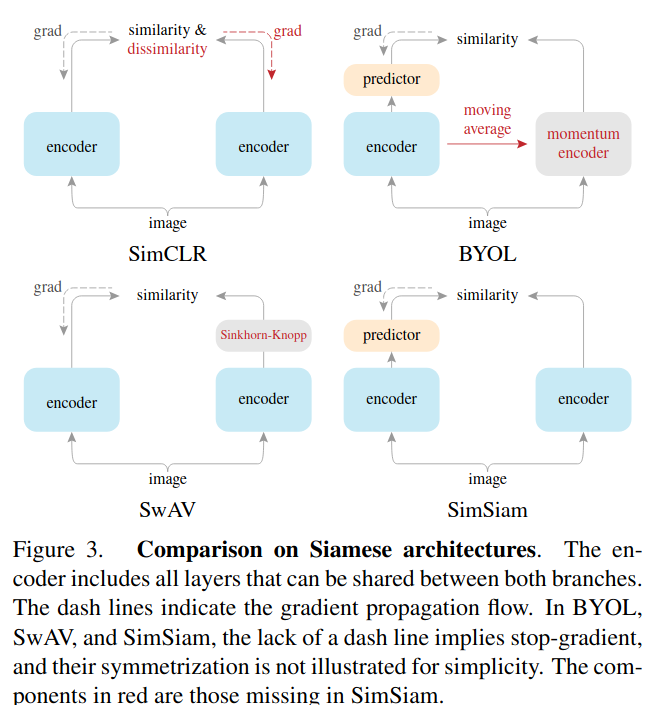
\includegraphics[width=\textwidth]{simsiam-comp.png}
\end{figure}
\subsection{Intuitions}

BYOL既没有使用negative samples, 但是使用了momentum encoder+不对称的proj. head+stop-grad策略来避免collapse, 并且不需要巨大的batchsize! 所以本方法可以考虑为BYOL-momentum encoder, 使用两个共享权重的网络(like SwAV without online clustering/SimCLR without negative pairs), 即使如此, 不会导致mode collapse!

\begin{remark}
    stop-grad是关键的, 没有stop-grad则会直接收敛到trivial解(mode collapse)
\end{remark}

\subsection{Method}

使用共享权重的backbone(like ResNet)+proj. head(MLP), 最小化不同视图最后特征的负cosine-sim.
\begin{equation}
    \mathcal{D}\left(p_{1}, z_{2}\right)=-\frac{p_{1}}{\left\|p_{1}\right\|_{2}} \cdot \frac{z_{2}}{\left\|z_{2}\right\|_{2}}
\end{equation}
并且使用对称化loss
\begin{equation}
    \mathcal{L}=\frac{1}{2} \mathcal{D}\left(p_{1}, z_{2}\right)+\frac{1}{2} \mathcal{D}\left(p_{2}, z_{1}\right)
\end{equation}
并且不对一边的网络进行参数更新.

\bt{Settings} \begin{itemize}
    \item Optimizer: SGD for pre-traininig. $lr=lr_{base}\times \text{BatchSize}/256$, base lr为0.05, 使用cosine decay(annealing) schedule, L2正则化1e-4, 动量0.9.
    \item Batch Size ~ 512, Synchronized BN across devices.
    \item Proj. Head: 3FCN of 2048-d.
    \item Pred. Head: 2FCN of 2048-512-2048-d.
\end{itemize}

\section{Graph Layouts by t-SNE}

\subsection{Backgrounds}

\bt{Dimension Reduction}

投影高维数据到低维, 可分为distance-preserving方法, 最小化(aggregated normalized) stress
\begin{equation}
    \sigma=\sum_{i, j}\left(\frac{d\left(\mathbf{x}_{i}, \mathbf{x}_{j}\right)-\left\|\mathbf{y}_{i}-\mathbf{y}_{j}\right\|}{d\left(\mathbf{x}_{i}, \mathbf{x}_{j}\right)}\right)^{2}
\end{equation}
以及neighborhood-preserving方法, 最大化kNN的重叠. distance-preserving方法在特别高维时失效很严重(由于高维空间的各种奇性).

\subsection{Method}
% !TODO
\subsection{tsNET}

\section{细粒度图像数据分类 by Xiangteng He}

困难: 标注成本巨大, 依赖人工先验, 忽略辨识速度(like RPN, 2-stages), 忽略语义关联

\subsection{细粒度图像数据分类}
    基于显著性图
\subsection{RL-based 图像部件/对象识别}
\subsection{多层注意力区域辨识}
    基于IoU的奖励函数强化学习
\subsection{多模态}
\begin{itemize}
    \item 引入文本信息,音频,视频
    \item 数据集构建 PKU FG-Xmedia
    \item ResNet-based统一处理各种模态, 视频抽帧, 音频使用mel谱图, 文本使用word embedding
\end{itemize}

Future: 大规模细粒度图像分类, 细粒度视觉推理, 图像到跨媒体迁移

\section{Dirac Operator for Extrinstic Shape Analysis}

为什么需要微分算子? 他们提供了一组流形上的基函数(Hilbert空间的基), 以及对应特征值. 流形上的函数可以在这些基上展开, 并且提供了傅立叶变换和卷积. 在紧流形上, 一个算子有离散的特征基, 若他是自伴和椭圆算子(矩阵为对称的和正定的). 然而很多微分算子并不满足这些条件:
\begin{itemize}
    \item Laplace-Beltrami Op., i.e. $\Delta$, 一种曲面光滑性的度量. 
    \item Hessian矩阵, 和modified Dirichlet能量. $\sum_i E_D(N^i\phi)$
    \item 各项异性Laplacian $\Delta_A=\operatorname{div} A \nabla$
\end{itemize}
对于曲面M, L算子可以看做Dirichlet能量的Hessian. 我们提出Dirac Op.

\subsection{Math}

使用四元数来表示曲面(的一个嵌入$f: M\mapsto \Im \mathbb H$). 假设这个嵌入是共形(conformal)的. 使用$\kappa_1, \kappa_2$代表两个主曲率, 有高斯曲率$K=\kappa_1\kappa_2$和平均曲率$H:=\frac{1}{2}\left(\kappa_{1}+\kappa_{2}\right)$. $|df|^2$代表嵌入f诱导的体积元.

对于实值函数, L算子是最低阶非平凡自伴椭圆算子. 对于复变函数, 则存在1-order微分算子: Dirac算子. 经典例子是Cauchy-Riemann(Poincare)算子$\bar \partial$, 以及微分形式上的Hodge-Dirac算子$\star d+d \star$.

我们使用的是extrinstic D-Op.
\begin{equation}
    D\psi := -\frac{df\wedge d\psi}{|df|^2}
\end{equation}
其中$|df|^2$的除法为应用2-形式的Hodge star算子.

平方, 有
\begin{equation}
    D^{2} \psi=\Delta \psi+\frac{d N \wedge d \psi}{|d f|^{2}}
\end{equation}

相对微分算子
\begin{equation}
    D_{f_{1}, f_{2}} \psi:=-\frac{d f_{2} \wedge d \psi}{\left|d f_{1}\right|^{2}}
\end{equation}

单参数内插
\begin{equation}
    L(\tau):=(1-\tau) \Delta+\tau D_{N}
\end{equation}

算子$D_N$只是半正定的. 但是增加一些L算子的部分就能成为强正定的. 这些算子和曲率也有一定关系, $\Delta=\Delta_{\R^2}e^{-2u}$, $u$是对数共形尺度因子, 且满足Yamabe方程$\Delta u=K$. 由于要最小化$\langle\langle\Delta \varphi, \varphi\rangle\rangle$, $\Delta \varphi$在有很大高斯曲率的地方会很小.

MDE(modified Dirichlet energy)也可写成
\begin{equation}
    E_{M D E}(\varphi)=\langle\langle\Delta \varphi, \varphi\rangle\rangle+\int_{M} \varphi^{2}\left(\kappa_{1}^{2}+\kappa_{2}^{2}\right) d A
\end{equation}
这意味着它的Hessian是$\Delta + U$, 后者是Willmore势能$U=\kappa_1^2+\kappa_2^2$, 这鼓励特征函数在曲率很大地方有小的方差.

\subsection{离散化}

对以一个2-流形的三角mesh $K=(V, E, F)$, 不同于连续的情况, 使用法向量N代替f. 对于任何mesh上的三角$ijk\in F$,$\psi:V\mapsto \mathbb H$ 有
\begin{equation}
    \left(D_{N} \psi\right)_{i j k}:=-\frac{1}{2 \mathcal{A}_{i j k}} \sum_{p q r \in \mathcal{C}(i j k)}\left(N_{r}-N_{q}\right) \psi_{p}
\end{equation}
其中$\mathcal A_{ijk}$是三角面积, $\mathcal C({ijk})$是轮换. 这个算子可以写成张量$D\in \mathbb H^{|F|\times |V|}$
\begin{equation}
    \mathrm{D}_{i j k, p}=-\left(N_{r}-N_{q}\right) / 2 \mathcal{A}_{i j k}
\end{equation}

\subsection{实值表示}
用4x4矩阵代替四元数运算. 为了找到典型表示, 需要找到乘积常数q,使得某个特征向量范数接近1.近似的有
\begin{equation}
    q:=\sum_{i=1}^{|V|} \mathcal{A}_{i} \phi_{i}^{-1}
\end{equation}
其中$A_i$是对偶区域的面积.

\subsection{有界区域: 边界条件}

边界条件可以是Dirichlet/Neumann条件. 这里提出无限势阱边界. 增加一个势能项U, 并且在有界区域之外迅速趋向无穷, 使得优化$\langle\{(\Delta+U) \psi, \psi\rangle\rangle$让波函数迅速在区域外收敛到0.
\begin{equation}
    U(p):=\frac{c}{1+\left(e^{-(d(p, q)-\beta)}\right)^{\gamma}}
\end{equation}
q是质心, c是大常数.

为了使用这个罚函数, 在算子中加入对角矩阵$U_{ii}=A_i U(p_i)$

\section{Mesh-Based Simulation with GNNs}
\begin{figure}[htbp]
    \centering
    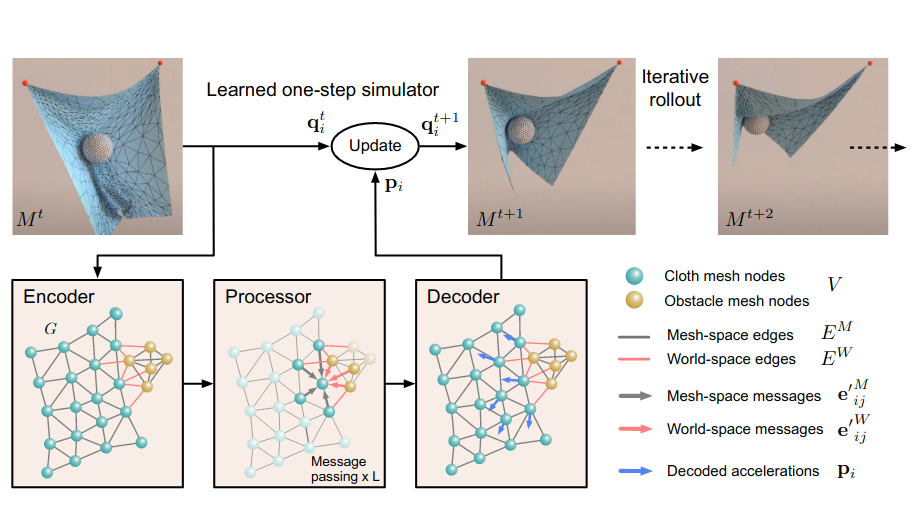
\includegraphics[width=\textwidth]{meshsim.png}
\end{figure}

使用World/Mesh两种空间的输入. 预测物理体系的时间序列. 使用$M^t=(V, E^M)$描述t时间的系统状态. 每个结点都有mesh-space坐标$\bm u_i$和是动量/速度坐标$\bm q_i$. 对于欧拉系统, 建模的是固定的mesh上的速度场, 对于Lagrange系统, mesh是动态移动的, 并且包含了绝对世界坐标$\bm x_i$. 

\subsection{结构}

Encoder: 把$M^t$编码成多重图$G=(V,E^M, E^W)$, 并且增加了世界坐标下的边$E^W$. 这里使用简单的rNN采样, 选取半径为最短的mesh边长$r_W$. 并且mesh图边权为相对坐标$\mathbf{u}_{i j}=\mathbf{u}_{i}-\mathbf{u}_{j}$ , 同理世界坐标图中也为相对坐标. 

Processor: GNN. 其中
\begin{align}
    \bs {e'}^{X}_{ij}=f^X(\bs e^{X}_{ij}, \bs v_i, \bs v_j)
\end{align}

Decoder: 使用在结点feature上的MLP. 得到输出向量$\bs p_i$

Updater: 对于一阶系统, $\mathbf{q}_{i}^{t+1}=\mathbf{p}_{i}+\mathbf{q}_{i}^{t}$, 二阶系统: $\mathbf{q}_{i}^{t+1}=\mathbf{p}_{i}+2 \mathbf{q}_{i}^{t}-\mathbf{q}^{t-1}$. 输出向量的额外维度也用于预测附加属性(压力/张力 etc.)

\subsection{Adaptive Remeshing}
\begin{figure}[htbp]
    \centering
    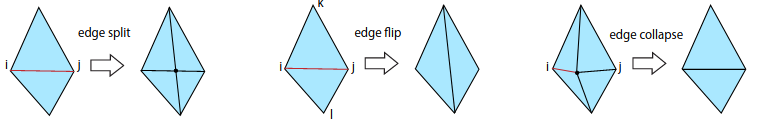
\includegraphics[width=\textwidth]{sizing.png}
\end{figure}
在需要的地方增加mesh数量.(有限元那味儿) 使用sizing filed方法. 定义sizing field张量$\mathbf{S}(\mathbf{u}) \in \mathbb{R}^{2 \times 2}$, 同时一条边是合理的iff. $\mathbf{u}_{i j}^{\mathrm{T}} \mathbf{S}_{i} \mathbf{u}_{i j} \leq 1$, 否则需要拆分这条边.

使用动态的remeshing. 使用如上文的GNN的结构来学习sizing张量场. 每一步, 我们都计算动量信息和resizing张量场, 再用remesher计算下一步的mesh.

给定了sizing张量场$\bs S_i$, 对于每条边, \begin{itemize}
    \item 需要分割, 若$\mathbf{u}_{i j}^{\mathrm{T}} \mathbf{S}_{i j} \mathbf{u}_{i j}>1$, $\mathbf{S}_{i j}=\frac{1}{2}\left(\mathbf{S}_{i}+\mathbf{S}_{j}\right)$
    \item 需要collapse, 若collapse不会产生新的无效边
    \item 需要flip, 若满足各项异性Delaunay条件\begin{equation}
        \left(\mathbf{u}_{j k} \times \mathbf{u}_{i k}\right) \mathbf{u}_{i l}^{T} \mathbf{S}_{A} \mathbf{u}_{j l}<\mathbf{u}_{j k}^{T} \mathbf{S}_{A} \mathbf{u}_{i k}\left(\mathbf{u}_{i l} \times \mathbf{u}_{j l}\right), \quad \mathbf{S}_{A}=\frac{1}{4}\left(\mathbf{S}_{i}+\mathbf{S}_{j}+\mathbf{S}_{k}+\mathbf{S}_{l}\right)
    \end{equation}
\end{itemize}
顺序上, 先尽可能split所有边, 再尽可能collapse所有边, 再尽可能flip所有边

若没有能估计sizing field的数据, 我们从mesh序列中估计之. 我们要找到能诱导出下一时刻mesh的sizing field. 假设remesher几乎是最优的, 所有结果边都有效, 那么最大化度规$\bm S$下的边长
\begin{equation}
    \mathbf{S}_{i}=\operatorname{argmax} \sum_{j \in \mathcal{N}_{i}} \mathbf{u}_{i j}^{\mathrm{T}} \mathbf{S}_{i} \mathbf{u}_{i j}, \quad \text { s.t. } \forall j \in \mathcal{N}_{i}: \mathbf{u}_{i j}^{\mathrm{T}} \mathbf{S}_{i} \mathbf{u}_{i j} \leq 1
\end{equation}
这是简单的凸优化(找到最小面积, 0-中心的包含$\bm u_{ij}$的椭圆).

\section{SENet}
Squeeze-and-Excitation Module.
\begin{figure}[htbp]
    \centering
    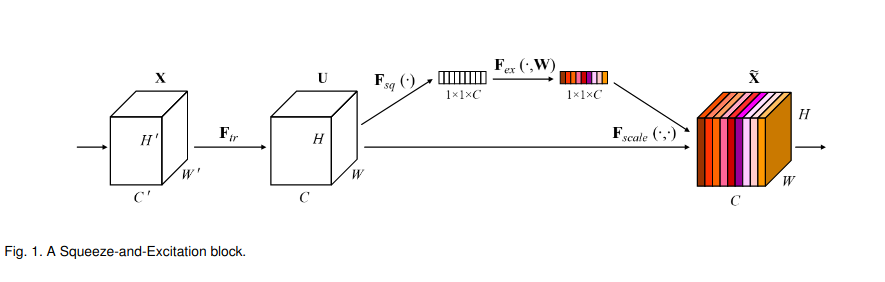
\includegraphics[width=\textwidth]{senet.png}
\end{figure}

计算squeeze变换(单纯的计算每个channel的均值)
\begin{equation}
    z_{c}=\mathbf{F}_{s q}\left(\mathbf{u}_{c}\right)=\frac{1}{H \times W} \sum_{i=1}^{H} \sum_{j=1}^{W} u_{c}(i, j)
\end{equation}

计算excitation, $\sigma$是sigmoid, $\delta$是ReLU
\begin{equation}
    \mathbf{s}=\mathbf{F}_{e x}(\mathbf{z}, \mathbf{W})=\sigma(g(\mathbf{z}, \mathbf{W}))=\sigma\left(\mathbf{W}_{2} \delta\left(\mathbf{W}_{1} \mathbf{z}\right)\right)
\end{equation}
其中$\mathbf{W}_{1} \in \mathbb{R}^{\frac{C}{r} \times C}$,  $\mathbf{W}_{2} \in \mathbb{R}^{C \times \frac{C}{r}}$维度形成某种bottleneck, 降低模型复杂度.

将excitation乘到channel上
\begin{equation}
    \widetilde{\mathbf{x}}_{c}=\mathbf{F}_{\text {scale }}\left(\mathbf{u}_{c}, s_{c}\right)=s_{c} \mathbf{u}_{c}
\end{equation}\footnote{
    in matrix-sense, 
    \begin{align}
        &\bs z=\frac 1 {HW} u_{ij}1^{ij} \in \R^{C\times 1}\\
        &\bs s=\bs F_{ex}(\bs z)\in \R^{C\times 1}\\
        &\widetilde{\bs X}=\bs s^T \odot \bs U \in {\R^{N(=H\times W)\times C}}
    \end{align}
}

\section{Continuous-Time Spiking Neural Network}

模拟真实神经元. alternative to Hebb 神经元. 传统的SNN模拟手段涉及时间驱动(time-driven)和事件驱动(event-driven), 前者涉及时间格点上的离散化, 可能带来误差. 采用event-driven来实现连续时间.

\subsection{Neurons}
\begin{equation}
    \begin{array}{l}
    S=S_{p}+P_{r} P_{w}-T_{l}, \text { for } S<S_{t h} \\
    S=S_{p}+P_{r} P_{w}+T_{r}, \text { for } S \geq S_{t h}
    \end{array}
\end{equation}
\begin{itemize}
    \item $S_p$, 之前的状态
    \item $P_r$: presynaptic weight, 受到的刺激
    \item $P_w$: postsynaptic weight, 神经元连接强度
    \item $T_l$: 电位leakage ~ $Ld\Delta t$
    \item $T_r$: $T_{r}=\frac{\left(S_{p}-1\right)^{2} \Delta t}{1-\left(S_{p}-1\right) \Delta t}$
    \item $t_f$: firing time, obeys firing equation $t_f=\frac 1 {S-1}$
\end{itemize}

可以有excitatory/inhibitory的输入区别.

\subsection{Network Topology}

一般来说, en比in多, 后者占网络的15-25\%, 这样可以增进网络的稳定性. 没有in-in突触, 这回导致不稳定性, 因为这会让in减少, 进而导致不受控制的激发.

\subsection{突触塑性规则}

"后突触规则": 是相对于同一突触的突触总体模式/时间点控制了后突触效用.

\begin{itemize}
    \item 对数衰减. 所有后突触权重postsynaptic weight对数衰减. 
    $$P_{w}=P_{w, \min }+\left(P_{w}-P_{w, \min }\right) \mathrm{e}^{-\frac{\Delta t}{\tau}}$$
    \item 同突触增强. 当一个spiking event在一个突触上发生, PW增加, 和同神经元+同突触的上一个刺激成函数(在一个时间窗口内).
    \item 异突触增强. 当一个spiking event在一个突触上发生, PW增加, 和同神经元+其他突触的上一个刺激成函数(在一个时间窗口内).
\end{itemize}

同/异突触增强使用以下方程控制. 
\begin{equation}
    \Delta P_{w}=\eta\left(P_{w, \max }-P_{w}\right)
\end{equation}

子后, 还可以采取其他策略, 如STDP, Synaptic Scaling etc.

\end{document}